% Options for packages loaded elsewhere
\PassOptionsToPackage{unicode}{hyperref}
\PassOptionsToPackage{hyphens}{url}
%
\documentclass[
]{book}
\usepackage{amsmath,amssymb}
\usepackage{lmodern}
\usepackage{iftex}
\ifPDFTeX
  \usepackage[T1]{fontenc}
  \usepackage[utf8]{inputenc}
  \usepackage{textcomp} % provide euro and other symbols
\else % if luatex or xetex
  \usepackage{unicode-math}
  \defaultfontfeatures{Scale=MatchLowercase}
  \defaultfontfeatures[\rmfamily]{Ligatures=TeX,Scale=1}
\fi
% Use upquote if available, for straight quotes in verbatim environments
\IfFileExists{upquote.sty}{\usepackage{upquote}}{}
\IfFileExists{microtype.sty}{% use microtype if available
  \usepackage[]{microtype}
  \UseMicrotypeSet[protrusion]{basicmath} % disable protrusion for tt fonts
}{}
\makeatletter
\@ifundefined{KOMAClassName}{% if non-KOMA class
  \IfFileExists{parskip.sty}{%
    \usepackage{parskip}
  }{% else
    \setlength{\parindent}{0pt}
    \setlength{\parskip}{6pt plus 2pt minus 1pt}}
}{% if KOMA class
  \KOMAoptions{parskip=half}}
\makeatother
\usepackage{xcolor}
\usepackage{color}
\usepackage{fancyvrb}
\newcommand{\VerbBar}{|}
\newcommand{\VERB}{\Verb[commandchars=\\\{\}]}
\DefineVerbatimEnvironment{Highlighting}{Verbatim}{commandchars=\\\{\}}
% Add ',fontsize=\small' for more characters per line
\usepackage{framed}
\definecolor{shadecolor}{RGB}{248,248,248}
\newenvironment{Shaded}{\begin{snugshade}}{\end{snugshade}}
\newcommand{\AlertTok}[1]{\textcolor[rgb]{0.94,0.16,0.16}{#1}}
\newcommand{\AnnotationTok}[1]{\textcolor[rgb]{0.56,0.35,0.01}{\textbf{\textit{#1}}}}
\newcommand{\AttributeTok}[1]{\textcolor[rgb]{0.77,0.63,0.00}{#1}}
\newcommand{\BaseNTok}[1]{\textcolor[rgb]{0.00,0.00,0.81}{#1}}
\newcommand{\BuiltInTok}[1]{#1}
\newcommand{\CharTok}[1]{\textcolor[rgb]{0.31,0.60,0.02}{#1}}
\newcommand{\CommentTok}[1]{\textcolor[rgb]{0.56,0.35,0.01}{\textit{#1}}}
\newcommand{\CommentVarTok}[1]{\textcolor[rgb]{0.56,0.35,0.01}{\textbf{\textit{#1}}}}
\newcommand{\ConstantTok}[1]{\textcolor[rgb]{0.00,0.00,0.00}{#1}}
\newcommand{\ControlFlowTok}[1]{\textcolor[rgb]{0.13,0.29,0.53}{\textbf{#1}}}
\newcommand{\DataTypeTok}[1]{\textcolor[rgb]{0.13,0.29,0.53}{#1}}
\newcommand{\DecValTok}[1]{\textcolor[rgb]{0.00,0.00,0.81}{#1}}
\newcommand{\DocumentationTok}[1]{\textcolor[rgb]{0.56,0.35,0.01}{\textbf{\textit{#1}}}}
\newcommand{\ErrorTok}[1]{\textcolor[rgb]{0.64,0.00,0.00}{\textbf{#1}}}
\newcommand{\ExtensionTok}[1]{#1}
\newcommand{\FloatTok}[1]{\textcolor[rgb]{0.00,0.00,0.81}{#1}}
\newcommand{\FunctionTok}[1]{\textcolor[rgb]{0.00,0.00,0.00}{#1}}
\newcommand{\ImportTok}[1]{#1}
\newcommand{\InformationTok}[1]{\textcolor[rgb]{0.56,0.35,0.01}{\textbf{\textit{#1}}}}
\newcommand{\KeywordTok}[1]{\textcolor[rgb]{0.13,0.29,0.53}{\textbf{#1}}}
\newcommand{\NormalTok}[1]{#1}
\newcommand{\OperatorTok}[1]{\textcolor[rgb]{0.81,0.36,0.00}{\textbf{#1}}}
\newcommand{\OtherTok}[1]{\textcolor[rgb]{0.56,0.35,0.01}{#1}}
\newcommand{\PreprocessorTok}[1]{\textcolor[rgb]{0.56,0.35,0.01}{\textit{#1}}}
\newcommand{\RegionMarkerTok}[1]{#1}
\newcommand{\SpecialCharTok}[1]{\textcolor[rgb]{0.00,0.00,0.00}{#1}}
\newcommand{\SpecialStringTok}[1]{\textcolor[rgb]{0.31,0.60,0.02}{#1}}
\newcommand{\StringTok}[1]{\textcolor[rgb]{0.31,0.60,0.02}{#1}}
\newcommand{\VariableTok}[1]{\textcolor[rgb]{0.00,0.00,0.00}{#1}}
\newcommand{\VerbatimStringTok}[1]{\textcolor[rgb]{0.31,0.60,0.02}{#1}}
\newcommand{\WarningTok}[1]{\textcolor[rgb]{0.56,0.35,0.01}{\textbf{\textit{#1}}}}
\usepackage{longtable,booktabs,array}
\usepackage{calc} % for calculating minipage widths
% Correct order of tables after \paragraph or \subparagraph
\usepackage{etoolbox}
\makeatletter
\patchcmd\longtable{\par}{\if@noskipsec\mbox{}\fi\par}{}{}
\makeatother
% Allow footnotes in longtable head/foot
\IfFileExists{footnotehyper.sty}{\usepackage{footnotehyper}}{\usepackage{footnote}}
\makesavenoteenv{longtable}
\usepackage{graphicx}
\makeatletter
\def\maxwidth{\ifdim\Gin@nat@width>\linewidth\linewidth\else\Gin@nat@width\fi}
\def\maxheight{\ifdim\Gin@nat@height>\textheight\textheight\else\Gin@nat@height\fi}
\makeatother
% Scale images if necessary, so that they will not overflow the page
% margins by default, and it is still possible to overwrite the defaults
% using explicit options in \includegraphics[width, height, ...]{}
\setkeys{Gin}{width=\maxwidth,height=\maxheight,keepaspectratio}
% Set default figure placement to htbp
\makeatletter
\def\fps@figure{htbp}
\makeatother
\setlength{\emergencystretch}{3em} % prevent overfull lines
\providecommand{\tightlist}{%
  \setlength{\itemsep}{0pt}\setlength{\parskip}{0pt}}
\setcounter{secnumdepth}{5}
\usepackage{booktabs}
\ifLuaTeX
  \usepackage{selnolig}  % disable illegal ligatures
\fi
\usepackage[]{natbib}
\bibliographystyle{apalike}
\IfFileExists{bookmark.sty}{\usepackage{bookmark}}{\usepackage{hyperref}}
\IfFileExists{xurl.sty}{\usepackage{xurl}}{} % add URL line breaks if available
\urlstyle{same} % disable monospaced font for URLs
\hypersetup{
  pdftitle={ReadingNotes: Have you read today's papers?},
  pdfauthor={Rongting Huang rthuang@connect.hku.hk},
  hidelinks,
  pdfcreator={LaTeX via pandoc}}

\title{ReadingNotes: Have you read today's papers?}
\author{Rongting Huang \href{mailto:rthuang@connect.hku.hk}{\nolinkurl{rthuang@connect.hku.hk}}}
\date{2025-02-26}

\begin{document}
\maketitle

{
\setcounter{tocdepth}{1}
\tableofcontents
}
\hypertarget{preface}{%
\chapter*{Preface}\label{preface}}
\addcontentsline{toc}{chapter}{Preface}

This book is for Rongting's daily reading notes.

\hypertarget{about-the-author}{%
\chapter*{About the author}\label{about-the-author}}
\addcontentsline{toc}{chapter}{About the author}

\begin{figure}
\centering

\includegraphics{./figs/Rongting/IMG-5393.jpg}
\caption{1}
\end{figure}

\begin{figure}
\centering

\includegraphics{./figs/Rongting/IMG-6316.PNG}
\caption{2}
\end{figure}

\begin{figure}
\centering

\includegraphics{./figs/Rongting/IMG-7418.JPG}
\caption{3}
\end{figure}

\begin{figure}
\centering

\includegraphics{./figs/Rongting/IMG-8010.JPG}
\caption{Keep moving}
\end{figure}

\hypertarget{research-topics}{%
\chapter*{Research topics}\label{research-topics}}
\addcontentsline{toc}{chapter}{Research topics}

\hypertarget{about-the-book}{%
\chapter*{About the book}\label{about-the-book}}
\addcontentsline{toc}{chapter}{About the book}

\textbf{Note}: to build this book, use the following script in R and follow the \href{https://bookdown.org/yihui/bookdown/}{bookdown mannual}:

\begin{verbatim}
bookdown::render_book("index.Rmd", "bookdown::gitbook")
\end{verbatim}

\hypertarget{intro}{%
\chapter{Introduction}\label{intro}}

You can label chapter and section titles using \texttt{\{\#label\}} after them, e.g., we can reference Chapter \ref{intro}. If you do not manually label them, there will be automatic labels anyway, e.g., Chapter \ref{methods}.

Figures and tables with captions will be placed in \texttt{figure} and \texttt{table} environments, respectively.

\begin{Shaded}
\begin{Highlighting}[]
\FunctionTok{par}\NormalTok{(}\AttributeTok{mar =} \FunctionTok{c}\NormalTok{(}\DecValTok{4}\NormalTok{, }\DecValTok{4}\NormalTok{, .}\DecValTok{1}\NormalTok{, .}\DecValTok{1}\NormalTok{))}
\FunctionTok{plot}\NormalTok{(pressure, }\AttributeTok{type =} \StringTok{\textquotesingle{}b\textquotesingle{}}\NormalTok{, }\AttributeTok{pch =} \DecValTok{19}\NormalTok{)}
\end{Highlighting}
\end{Shaded}

\begin{figure}

{\centering 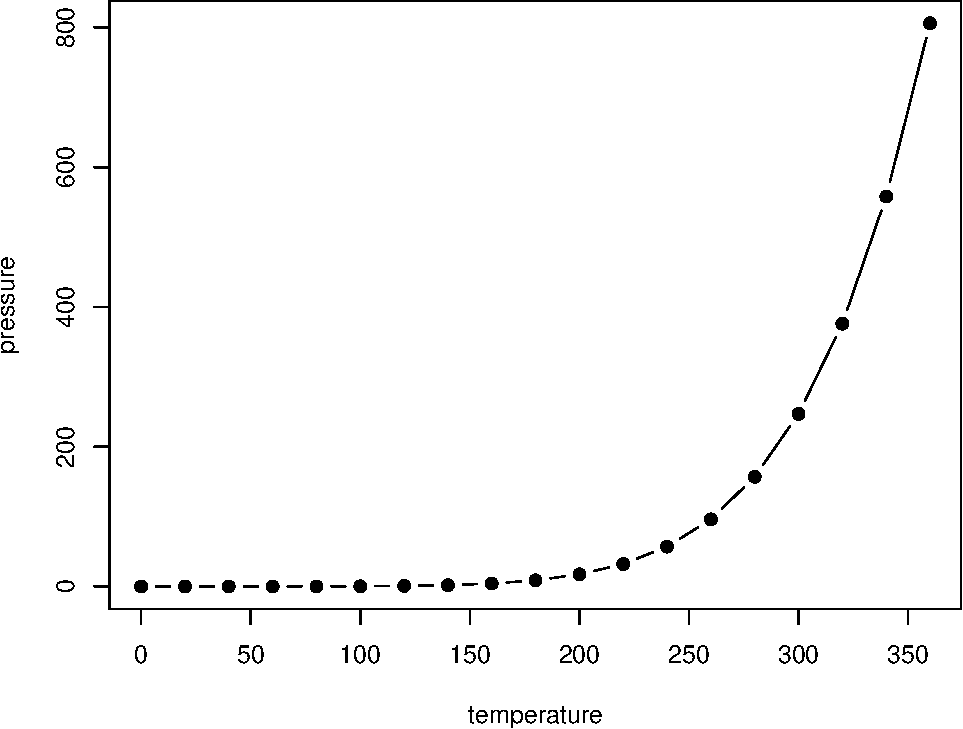
\includegraphics[width=0.8\linewidth]{ReadingNotes_files/figure-latex/nice-fig-1} 

}

\caption{Here is a nice figure!}\label{fig:nice-fig}
\end{figure}

Reference a figure by its code chunk label with the \texttt{fig:} prefix, e.g., see Figure \ref{fig:nice-fig}. Similarly, you can reference tables generated from \texttt{knitr::kable()}, e.g., see Table \ref{tab:nice-tab}.

\begin{Shaded}
\begin{Highlighting}[]
\NormalTok{knitr}\SpecialCharTok{::}\FunctionTok{kable}\NormalTok{(}
  \FunctionTok{head}\NormalTok{(iris, }\DecValTok{20}\NormalTok{), }\AttributeTok{caption =} \StringTok{\textquotesingle{}Here is a nice table!\textquotesingle{}}\NormalTok{,}
  \AttributeTok{booktabs =} \ConstantTok{TRUE}
\NormalTok{)}
\end{Highlighting}
\end{Shaded}

\begin{table}

\caption{\label{tab:nice-tab}Here is a nice table!}
\centering
\begin{tabular}[t]{rrrrl}
\toprule
Sepal.Length & Sepal.Width & Petal.Length & Petal.Width & Species\\
\midrule
5.1 & 3.5 & 1.4 & 0.2 & setosa\\
4.9 & 3.0 & 1.4 & 0.2 & setosa\\
4.7 & 3.2 & 1.3 & 0.2 & setosa\\
4.6 & 3.1 & 1.5 & 0.2 & setosa\\
5.0 & 3.6 & 1.4 & 0.2 & setosa\\
\addlinespace
5.4 & 3.9 & 1.7 & 0.4 & setosa\\
4.6 & 3.4 & 1.4 & 0.3 & setosa\\
5.0 & 3.4 & 1.5 & 0.2 & setosa\\
4.4 & 2.9 & 1.4 & 0.2 & setosa\\
4.9 & 3.1 & 1.5 & 0.1 & setosa\\
\addlinespace
5.4 & 3.7 & 1.5 & 0.2 & setosa\\
4.8 & 3.4 & 1.6 & 0.2 & setosa\\
4.8 & 3.0 & 1.4 & 0.1 & setosa\\
4.3 & 3.0 & 1.1 & 0.1 & setosa\\
5.8 & 4.0 & 1.2 & 0.2 & setosa\\
\addlinespace
5.7 & 4.4 & 1.5 & 0.4 & setosa\\
5.4 & 3.9 & 1.3 & 0.4 & setosa\\
5.1 & 3.5 & 1.4 & 0.3 & setosa\\
5.7 & 3.8 & 1.7 & 0.3 & setosa\\
5.1 & 3.8 & 1.5 & 0.3 & setosa\\
\bottomrule
\end{tabular}
\end{table}

You can write citations, too. For example, we are using the \textbf{bookdown} package \citep{R-bookdown} in this sample book, which was built on top of R Markdown and \textbf{knitr} \citep{xie2015}.

\hypertarget{sgcell}{%
\chapter{SingleCell}\label{sgcell}}

\hypertarget{technology}{%
\section{Technology}\label{technology}}

\hypertarget{single-cell}{%
\subsection{single cell}\label{single-cell}}

\begin{itemize}
\tightlist
\item
  scDNA
\item
  scRNA
\item
  scATAC
\end{itemize}

\hypertarget{spatial-single-cell}{%
\subsection{spatial single cell}\label{spatial-single-cell}}

\hypertarget{review}{%
\section{Review}\label{review}}

\hypertarget{review-2021-06}{%
\subsection{Review-2021-06}\label{review-2021-06}}

\href{https://www.nature.com/articles/s41592-021-01171-x}{The triumphs and limitations of computational methods for scRNA-seq}\citep{kharchenko2021triumphs}

Though computational approaches vary, most formulate (1) a statistical model of the measurement, (2) a representation of the data in reduced dimensions, and (3) an approximation of the expression manifold (Box 2), with a set of discrete transcriptional subpopulations being the simplest and the most common approximation. The problems motivating these steps, and the specific solutions and their assumptions, are the subject of this review.

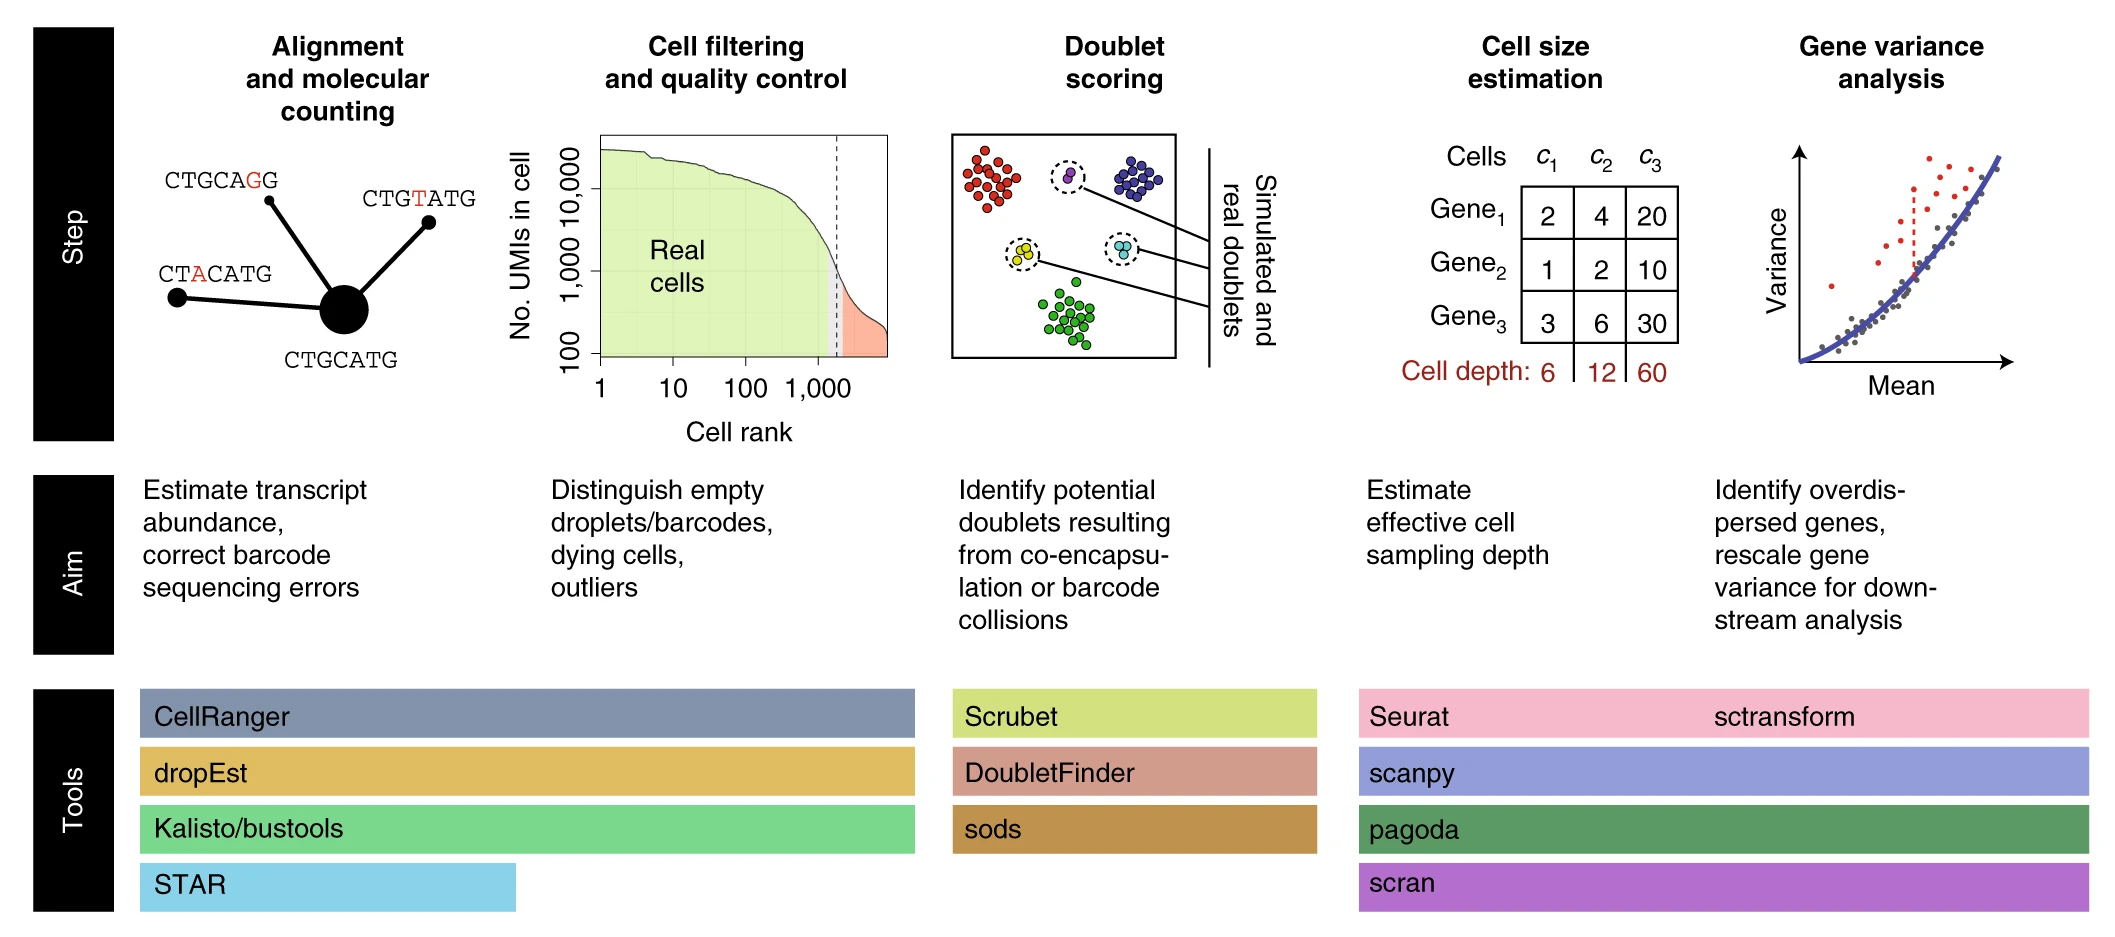
\includegraphics{./figs/singleCell/preprocessing_review1.jpg}
\href{https://www.nature.com/articles/s41592-021-01171-x/figures/1}{Key preprocessing steps in single-cell RNA-seq analysis}

\begin{figure}
\centering
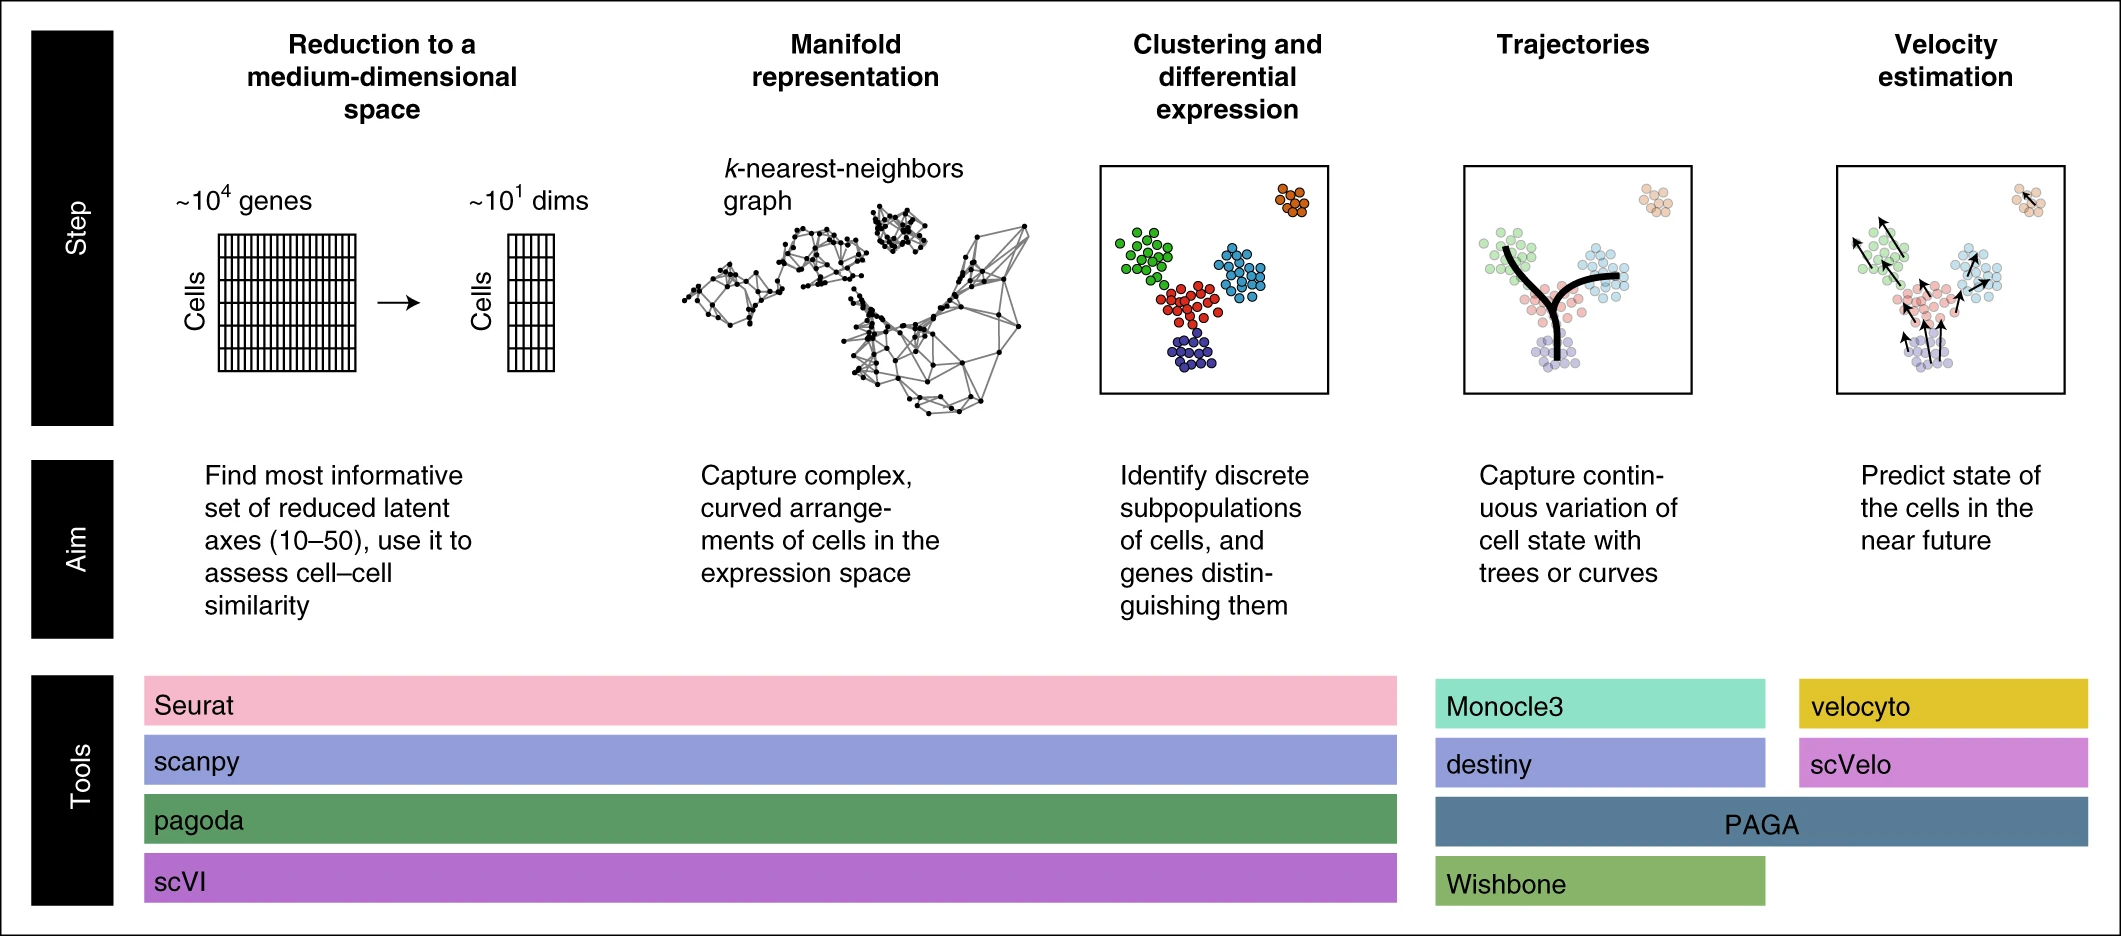
\includegraphics{./figs/singleCell/key_analysis_review2.jpg}
\caption{Key analysis steps in single-cell RNA-seq analysis}
\end{figure}

\href{https://www.nature.com/articles/s41592-021-01171-x/figures/2}{Key analysis steps in single-cell RNA-seq analysis}

\textbf{Box 1 Select software tools}
Tools for alignment, barcode correction, count matrix estimation, and quality control include:

\begin{itemize}
\item
  CellRanger (\url{https://support.10xgenomics.com/single-cell-gene-expression/software/pipelines/latest/installation}): supports 10x Chromium datasets (commercial product)
\item
  dropEst (\url{https://github.com/hms-dbmi/dropEst}): supports multiple droplet-based protocols
\item
  STAR (\url{https://github.com/alexdobin/STAR}): aligner (used internally by CellRanger and dropEst), also has built-in options for count matrix estimation
\item
  Optimus (\url{https://data.humancellatlas.org/pipelines/optimus-workflow}): supports 10x Chromium v2 and v3 datasets, designed for Human Cell Atlas
\item
  Kallisto/bustools (\url{https://www.kallistobus.tools}): fast processing using pseudoalignment
\end{itemize}

Cell filter and doublet identification tools include:

\begin{itemize}
\item
  EmptyDrops (\url{https://rdrr.io/github/MarioniLab/DropletUtils/man/emptyDrops.html}): uses a classifier to distinguish `empty' cells that look like the low-end tail of the cell size distribution
\item
  Scrublet (\url{https://github.com/AllonKleinLab/scrublet}): python-based, doublet simulation and doublet scoring
\item
  doubletFinder (\url{https://github.com/chris-mcginnis-ucsf/DoubletFinder}): R-based, doublet simulation and doublet scoring
\item
  scds (\url{https://github.com/kostkalab/scds}): fast doublet scoring implementation
\end{itemize}

Tools for normalization, dimensionality reduction, and clustering and differential expression include:

\begin{itemize}
\item
  Seurat (\url{https://satijalab.org/seurat/}): the most popular analysis toolkit, R-based
\item
  scanpy (\url{https://github.com/theislab/scanpy}): the most popular python-based toolkit
\item
  scVI (\url{https://github.com/YosefLab/scVI}): latent space identification using variational neural net
\item
  pagoda2 (\url{https://github.com/hms-dbmi/pagoda2}): fast, R-based processing
\item
  SAUCIE (\url{https://www.krishnaswamylab.org/projects/saucie}): a neural-net-based dimensionality reduction, using maximal mean discrepancy penalty
\end{itemize}

Tools for trajectory fitting include:

\begin{itemize}
\item
  Monocle3 (\url{https://cole-trapnell-lab.github.io/monocle3/}): third iteration of the Monocle package, including updated tree utilities
\item
  Slingshot (\url{https://github.com/kstreet13/slingshot}): tree fitting with improved pseudotime estimation
\item
  PAGA (\url{https://github.com/theislab/paga}): tree/graph fitting approach combined with cell aggregation, also supports cluster-based velocity estimates
\item
  Wishbone (\url{https://dpeerlab.github.io/dpeerlab-website/wishbone.html}): a bifurcation analysis method
\item
  Destiny, DPT (\url{https://github.com/theislab/destiny/}): dimensionality reduction and trajectory fitting using diffusion maps82
\end{itemize}

Tools for velocity estimation include:

\begin{itemize}
\item
  velocyto (\url{http://velocyto.org/}): reference python/R implementation
\item
  scVelo (\url{https://scvelo.readthedocs.io/}): new implementation using curve-based phase portrait fit
\end{itemize}

\hypertarget{statistical-view-of-a-cell}{%
\subsubsection{Statistical view of a cell}\label{statistical-view-of-a-cell}}

\hypertarget{comparing-transcriptional-states}{%
\subsubsection{Comparing transcriptional states}\label{comparing-transcriptional-states}}

\hypertarget{the-quest-for-reduced-dimensions}{%
\subsubsection{The quest for reduced dimensions}\label{the-quest-for-reduced-dimensions}}

\hypertarget{section}{%
\subsubsection{}\label{section}}

\begin{figure}
\centering
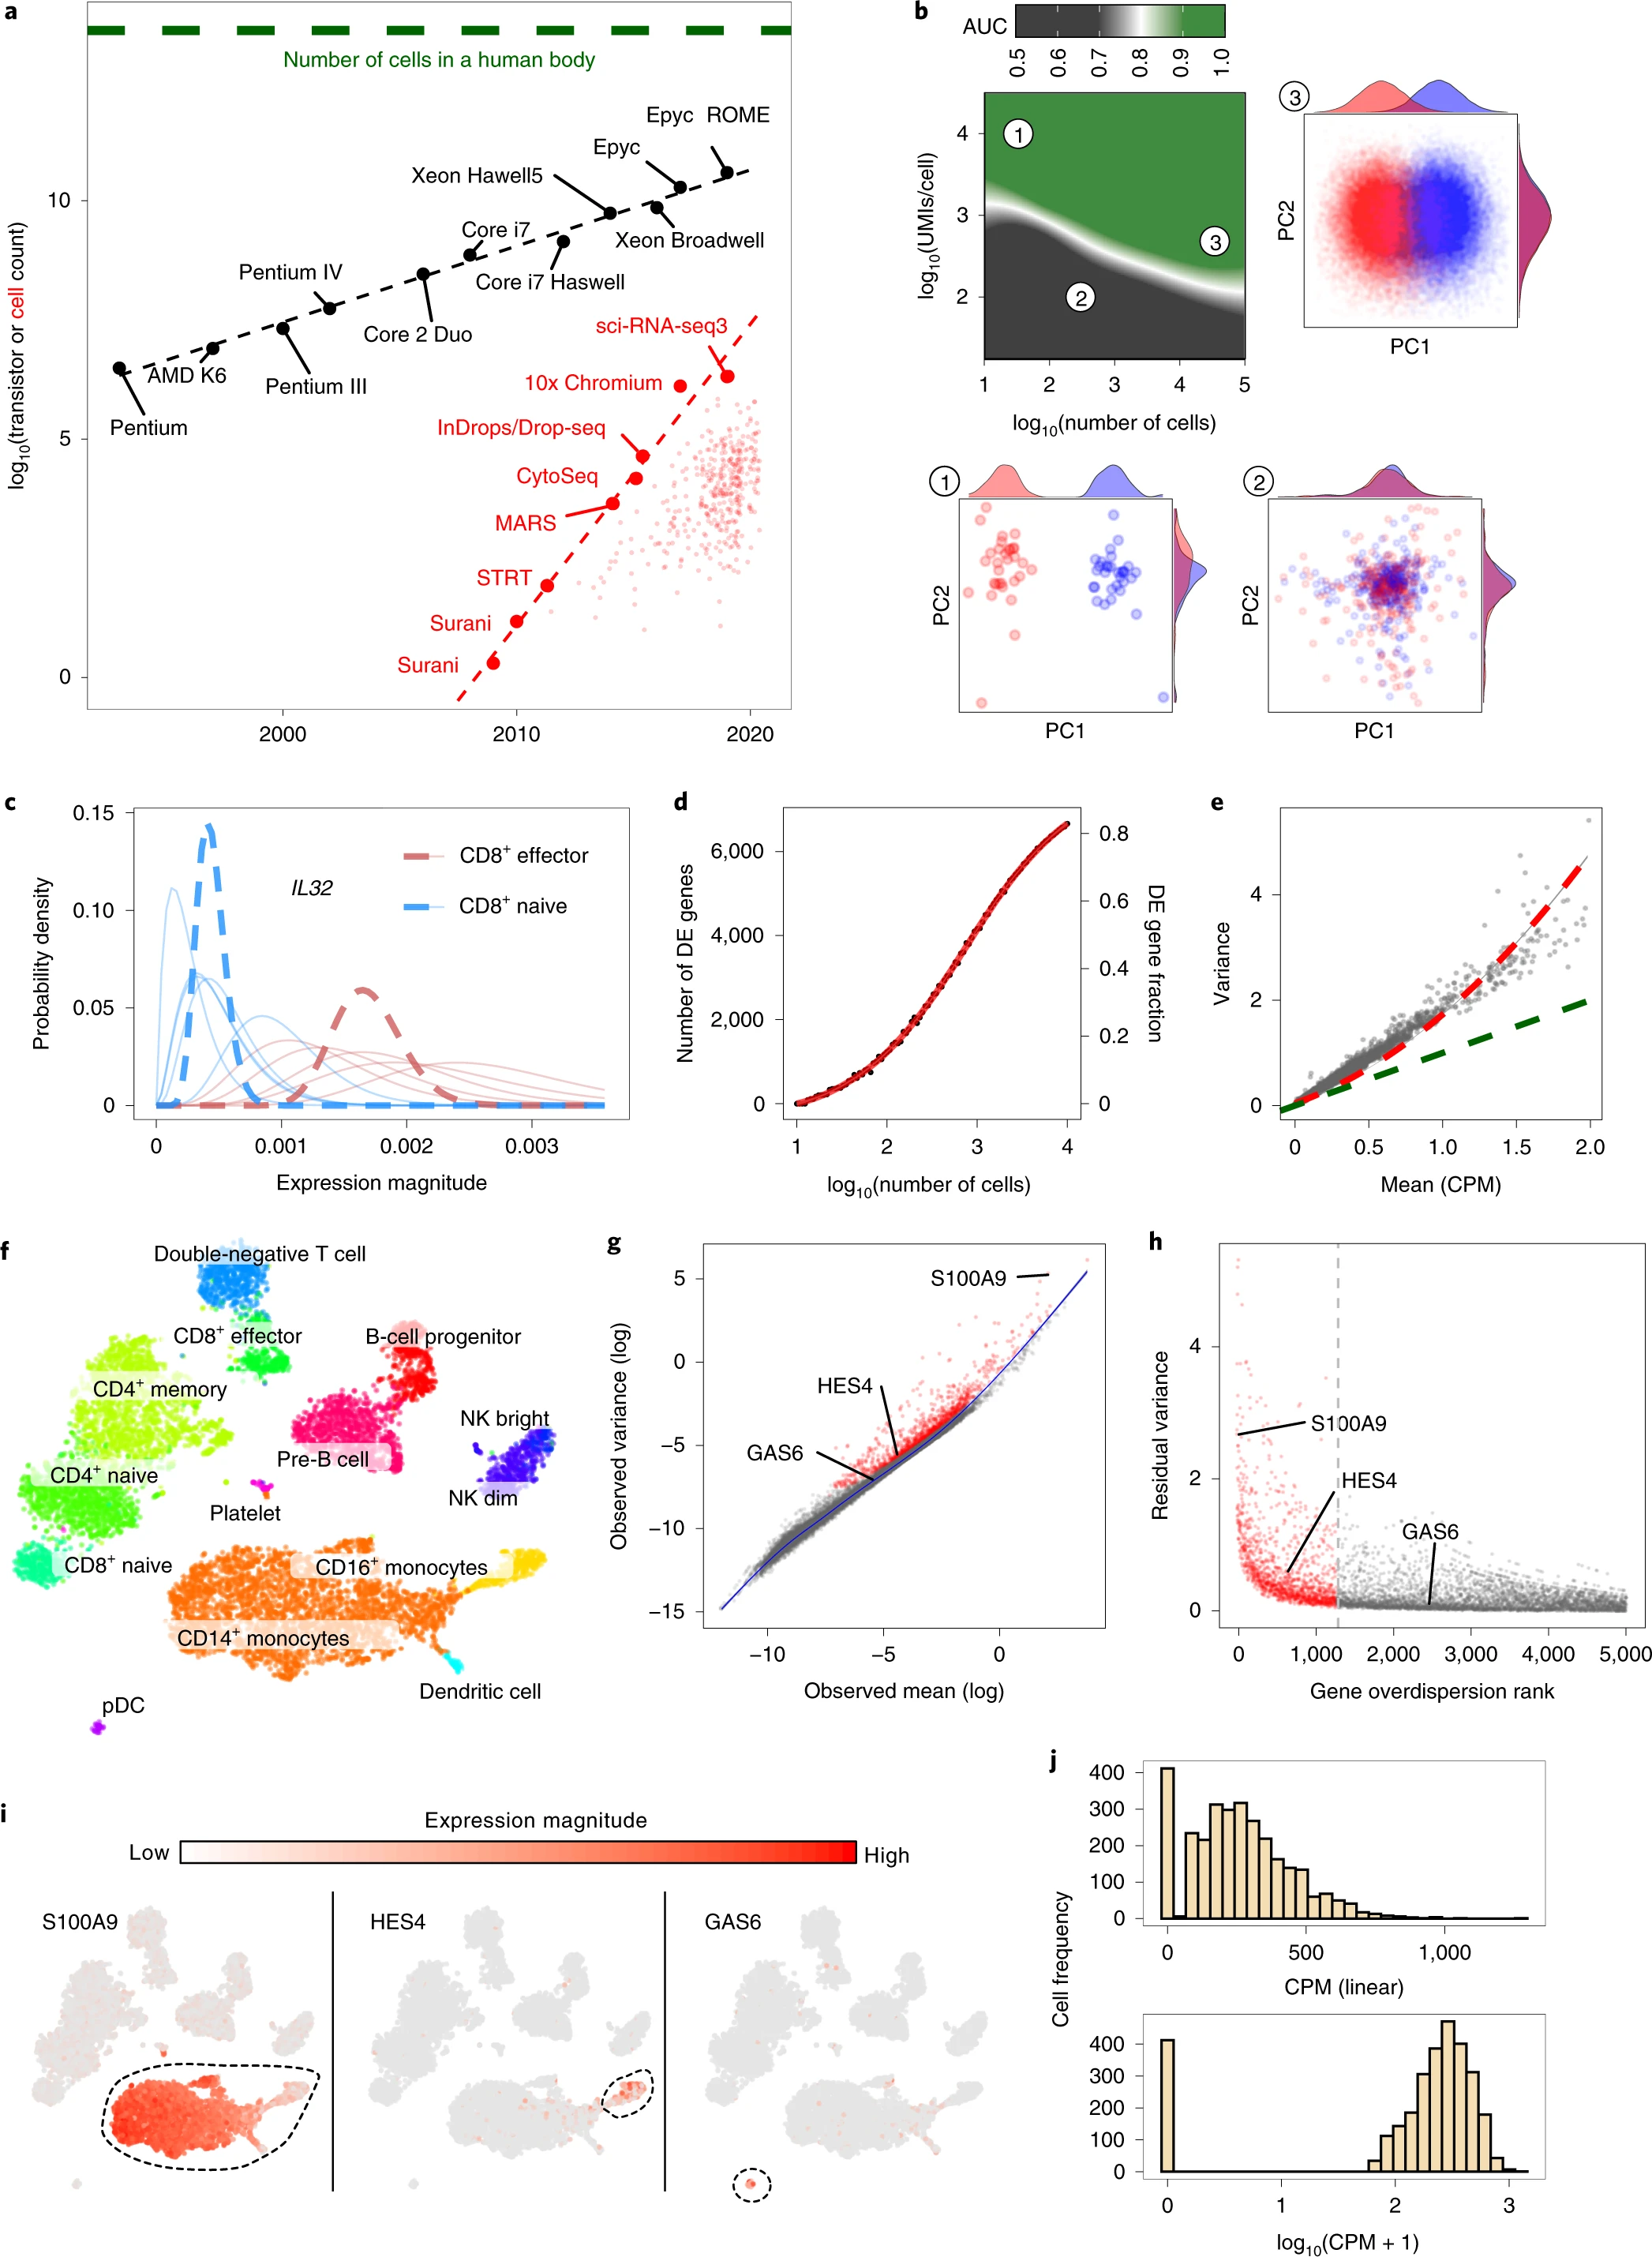
\includegraphics{./figs/singleCell/scRNA-seq basics.jpg}
\caption{scRNA-seq basics}
\end{figure}

\href{https://www.nature.com/articles/s41592-021-01171-x/figures/3}{scRNA-seq basics}

a, Beating Moore's law. The number of cells measured by landmark scRNA-seq datasets over years (red), compared with the increase in the CPU transistor counts (black). The set of all published scRNA-seq studies83 is shown with small red dots. The estimated number of cells in a human body is shown by a green dashed line.
b, Shallow coverage of each cell can be compensated for by measuring more cells. The ability to distinguish two cell populations, assessed by the area under the receiver operating characteristic curve (ROC AUC) measure, is shown as a function of the number of measured cells (x axis) and the mean cell depth (y axis). Examples of three different simulations (1-3) within different parts of this design parameter space are shown on PCA projections.
c, Probabilistic view of scRNA-seq estimates. Posterior probability of IL32 gene expression magnitude is shown for five cells from two different CD8+ T cell populations (red and blue, thin lines). Joint posteriors assessing the mean expression magnitude within each subpopulation are shown by thick dashed lines.
d, Comparing CD4+ T cells and CD14+ monocytes, the plot shows the number (y axis, left) and the fraction (y axis, right) of the genes passing a 1\% statistical significance threshold for differential expression (DE) as a function of the number of cells compared from each population (x axis).
e, The scatter plot shows for each gene (dots) the mean (x axis) and variance (y axis) of the normalized UMI counts (CPM, counts per million) in CD4+ T cells. The Poisson expected value is shown in green, with a quadratic-based negative binomial fit shown in red. f-i, Variance normalization and most variable genes.
f, A t-SNE embedding of a primary peripheral blood mononuclear cell (PBMC) dataset with cell annotations. NK, natural killer, separated into CD56 bright and dim subsets. pDC, plasmacytoid dendritic cell.
g, Mean-variance relationship of different genes (dots) in the PBMC dataset is shown for log-transformed expression estimates. The genome-wide relationship, as captured by smoothed regression, is shown by the blue line. Genes whose variance is significantly higher than the genome-wide trend are shown as red dots.
h, Residual variance is shown for the top 5,000 overdispersed genes, ordered by the statistical significance (x axis).
i, Expression pattern of several example genes, with circles highlighting the subpopulations distinguished by the genes.
j, Distribution of normalized expression magnitudes (CPM) for the CTSH gene across all CD14+ monocytes is shown on the linear scale (top) and after log transformation (bottom) with a pseudocount.

\hypertarget{review-2021-07}{%
\subsection{Review-2021-07}\label{review-2021-07}}

\href{https://www.nature.com/articles/s41587-021-00895-7}{Computational principles and challenges in single-cell data integration}\citep{argelaguet2021computational}

\hypertarget{review-2021-10}{%
\subsection{Review-2021-10}\label{review-2021-10}}

\href{https://genomebiology.biomedcentral.com/articles/10.1186/s13059-021-02519-4}{Over 1000 tools reveal trends in the single-cell RNA-seq analysis landscape}\citep{zappia2021over}

Single-cell gene expression measurements are cell type-specific (unlike DNA), more easily interpretable (compared to epigenetic modalities), and scalable to thousands of features (unlike antibody-based protein measurements) and thousands of cells. These features mean that scRNA-seq can be used as an anchor, often measured in parallel and used to link other modalities.

\href{https://github.com/Rongtingting/awesome-single-cell}{The Awesome Single Cell repository} is a community-curated list of software packages, resources, researchers, and publications for various single-cell technologies and \href{https://docs.google.com/spreadsheets/d/1IPe2ozb1Mny8sLvJaSE57RJr3oruiBoSudAVhSH-O8M/edit?pli=1\#gid=237186399}{Albert Villela's SingleCell Omics spreadsheet} tracks a range of information including technologies, companies, and software tools.

The scRNA-tools database focuses specifically on the cataloging and manual curation of software tools for analyzing scRNA-seq data {[}23{]}. When tools become available (usually through a bioRxiv preprint), we classify them according to the analysis tasks they can be used for and record information such as associated preprints and publications, software licenses, code location, software repositories, and a short description. Most tools are added to the database within 30 days of the first preprint or publication (Additional file 1: Figure S1). All the recorded information is publicly available in an interactive format at \url{https://www.scrna-tools.org/} {[}24{]}. As the number of tools in the database has moved past 1000, we have taken this opportunity to provide an update on the current state of the database and explore trends in scRNA-seq analysis across the past 5 years. We find that the focus of tool developers has moved on from continuous ordering of cells to methods for integrating samples and classifying cells. The database also shows us that more new tools are built using Python while the relative usage of R is declining. We also examine the role of open science in the development of the field and find that open source practices lead to increased citations. While the scRNA-tools database does not record every scRNA-seq analysis tool, the large proportion it does include over the history of what is still a young field make these analyses possible and a reasonable estimate of trends across all tools.

\hypertarget{data-processing}{%
\section{Data processing}\label{data-processing}}

\href{https://www.nature.com/articles/s41587-021-00875-x}{Bayesian inference of gene expression states from single-cell RNA-seq data}\citep{breda2021bayesian}

\href{https://www.nature.com/articles/s41587-021-00875-x/figures/1}{summary of sanity approach}

\begin{figure}
\centering
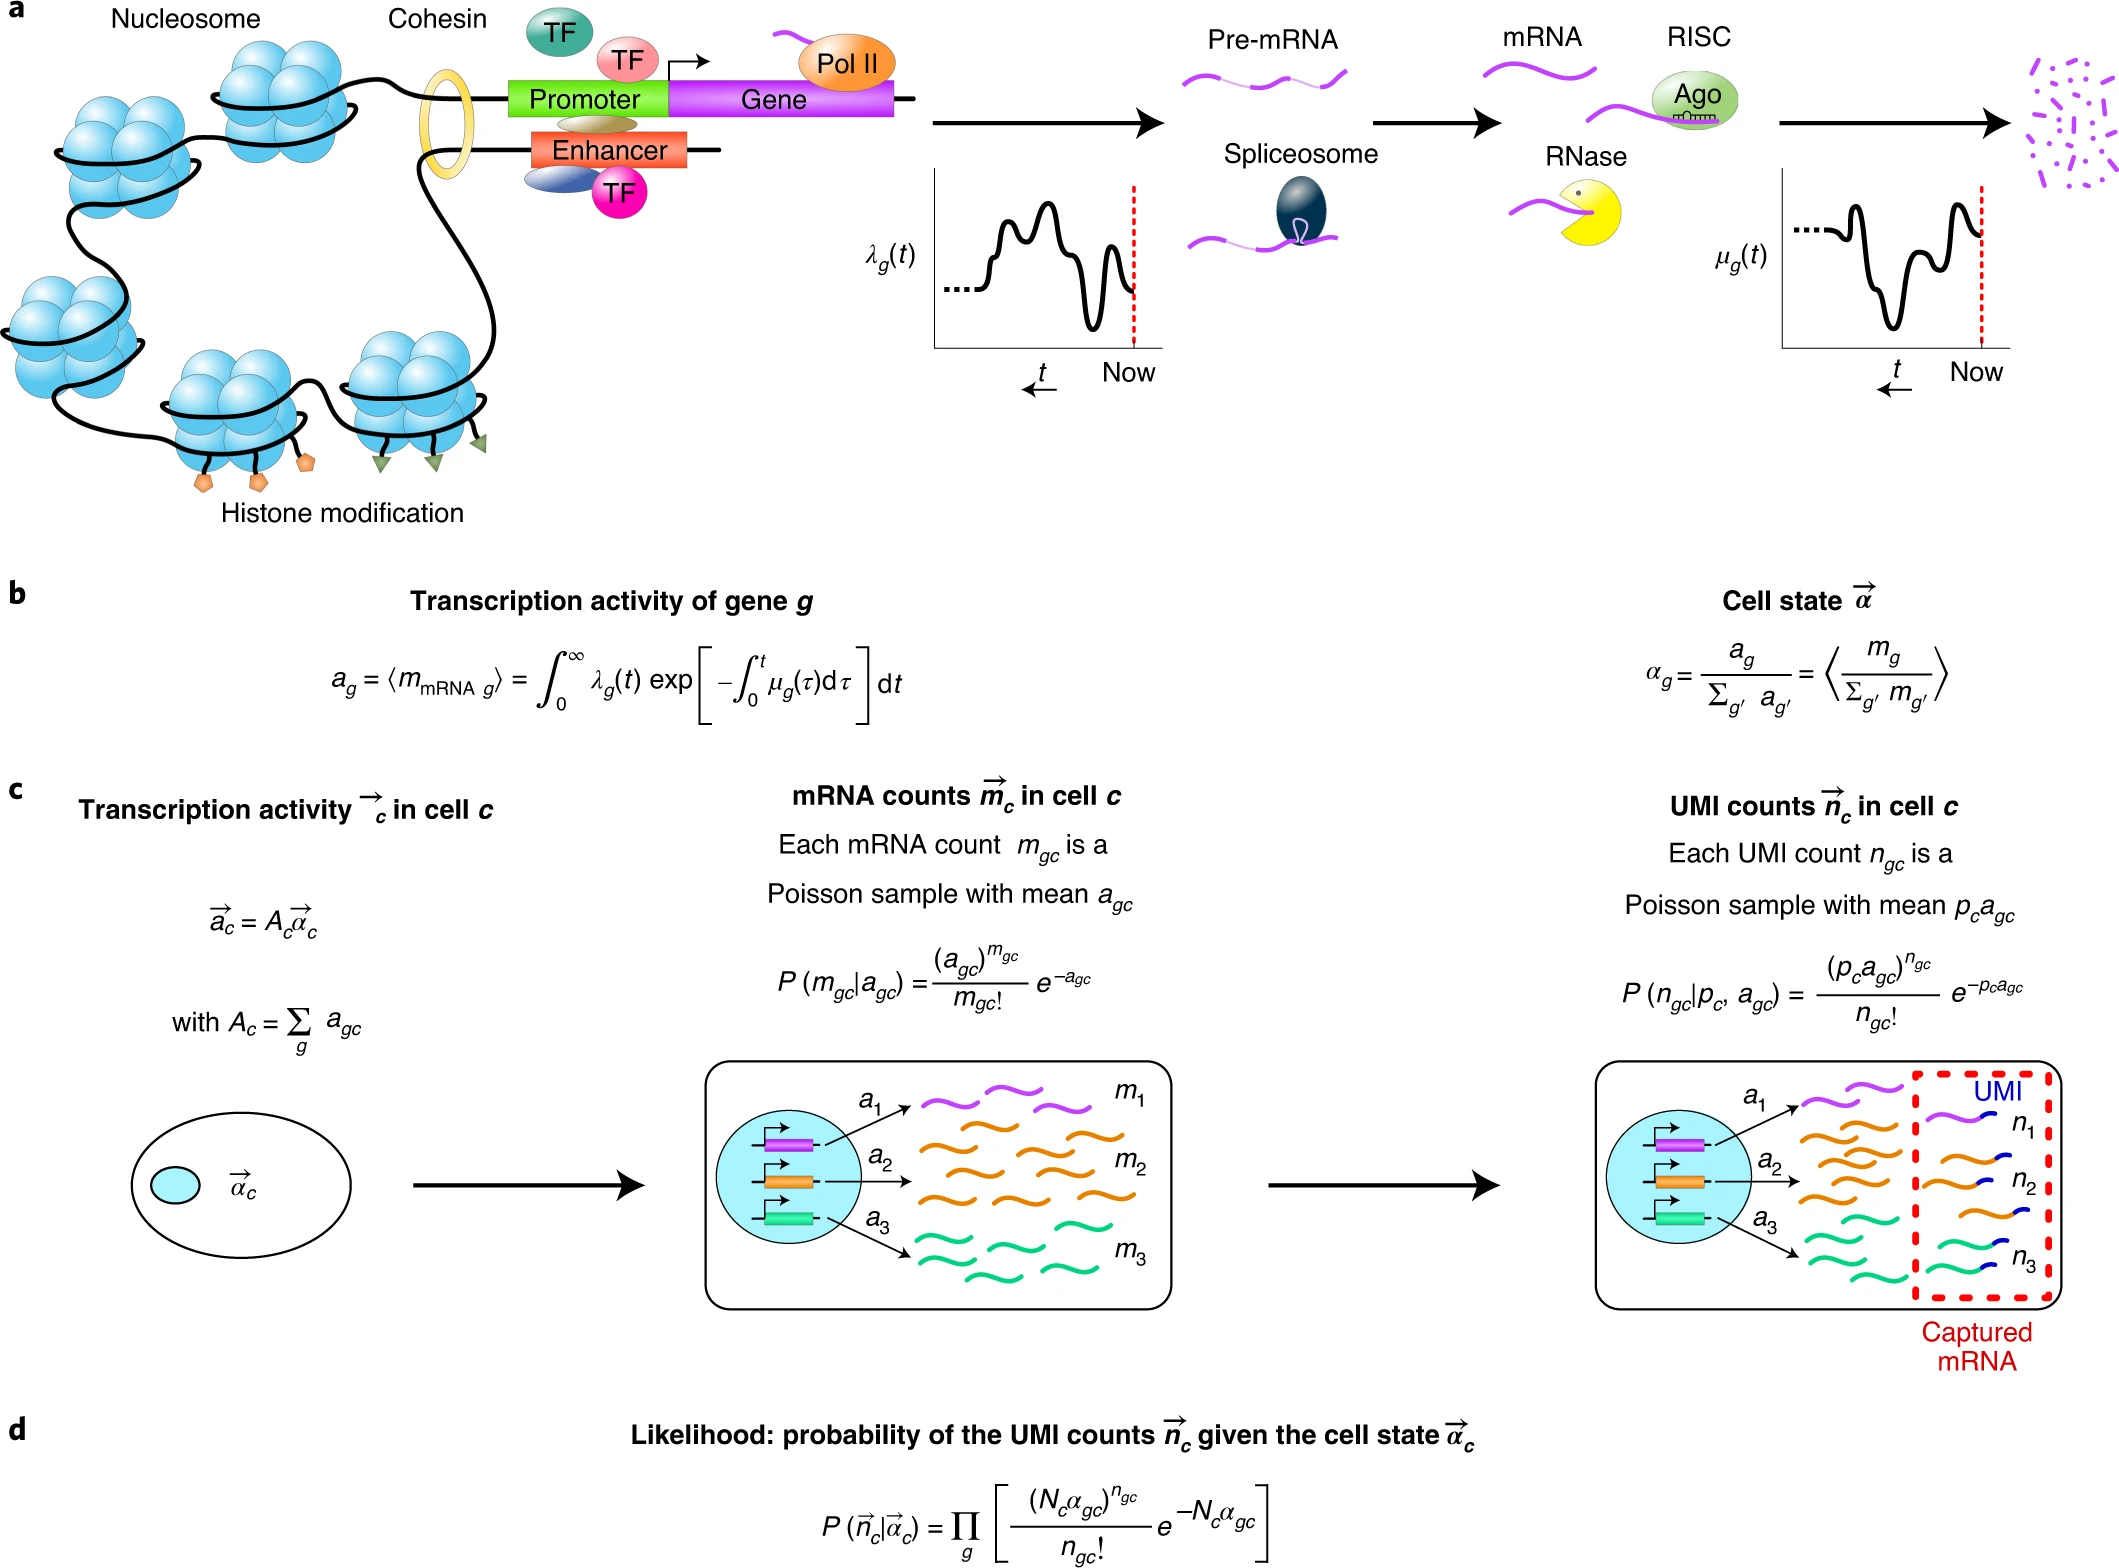
\includegraphics{./figs/singleCell/summary_Sanity.jpg}
\caption{summary of sanity approach}
\end{figure}

\begin{figure}
\centering
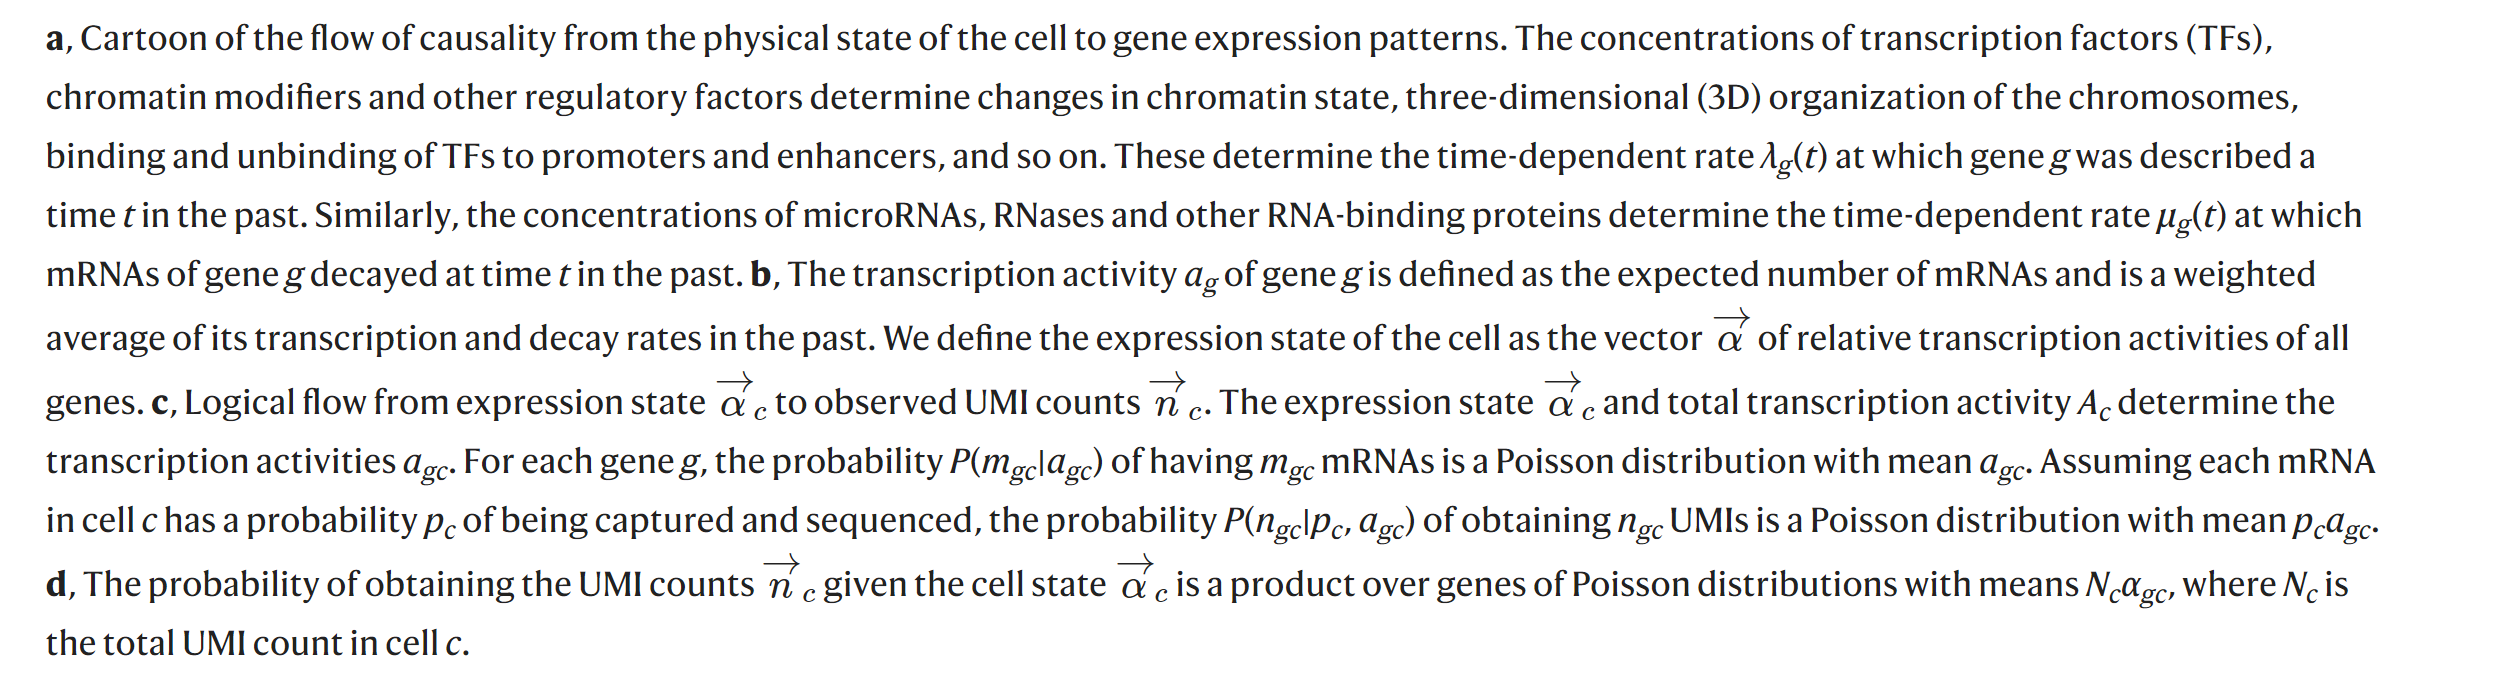
\includegraphics{./figs/singleCell/sanity_notes.png}
\caption{sanity notes}
\end{figure}

\hypertarget{clustering-methods}{%
\section{Clustering methods}\label{clustering-methods}}

\hypertarget{benchmarking}{%
\section{Benchmarking}\label{benchmarking}}

\href{https://www.nature.com/articles/s41592-021-01336-8}{Benchmarking atlas-level data integration in single-cell genomics}\citep{luecken2021benchmarking}

\begin{figure}
\centering
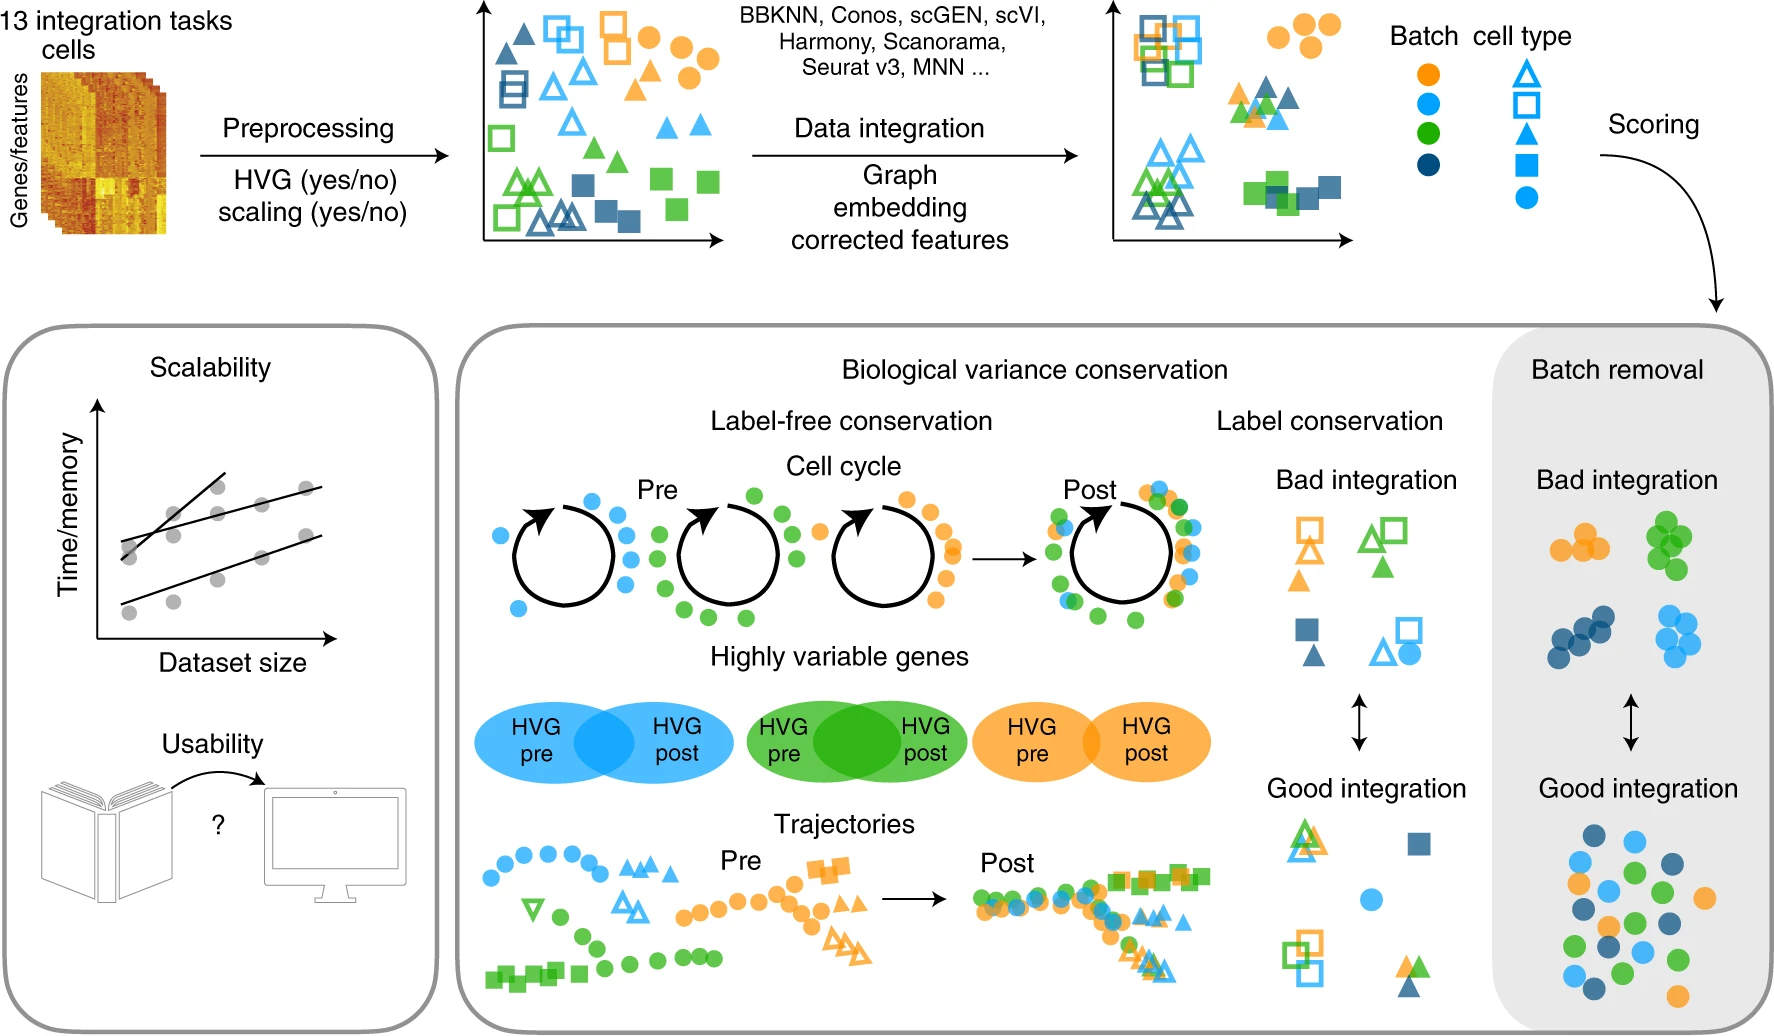
\includegraphics{./figs/singleCell/benchmarking1.jpg}
\caption{Design of single-cell integration benchmarking (scIB).}
\end{figure}

\begin{figure}
\centering
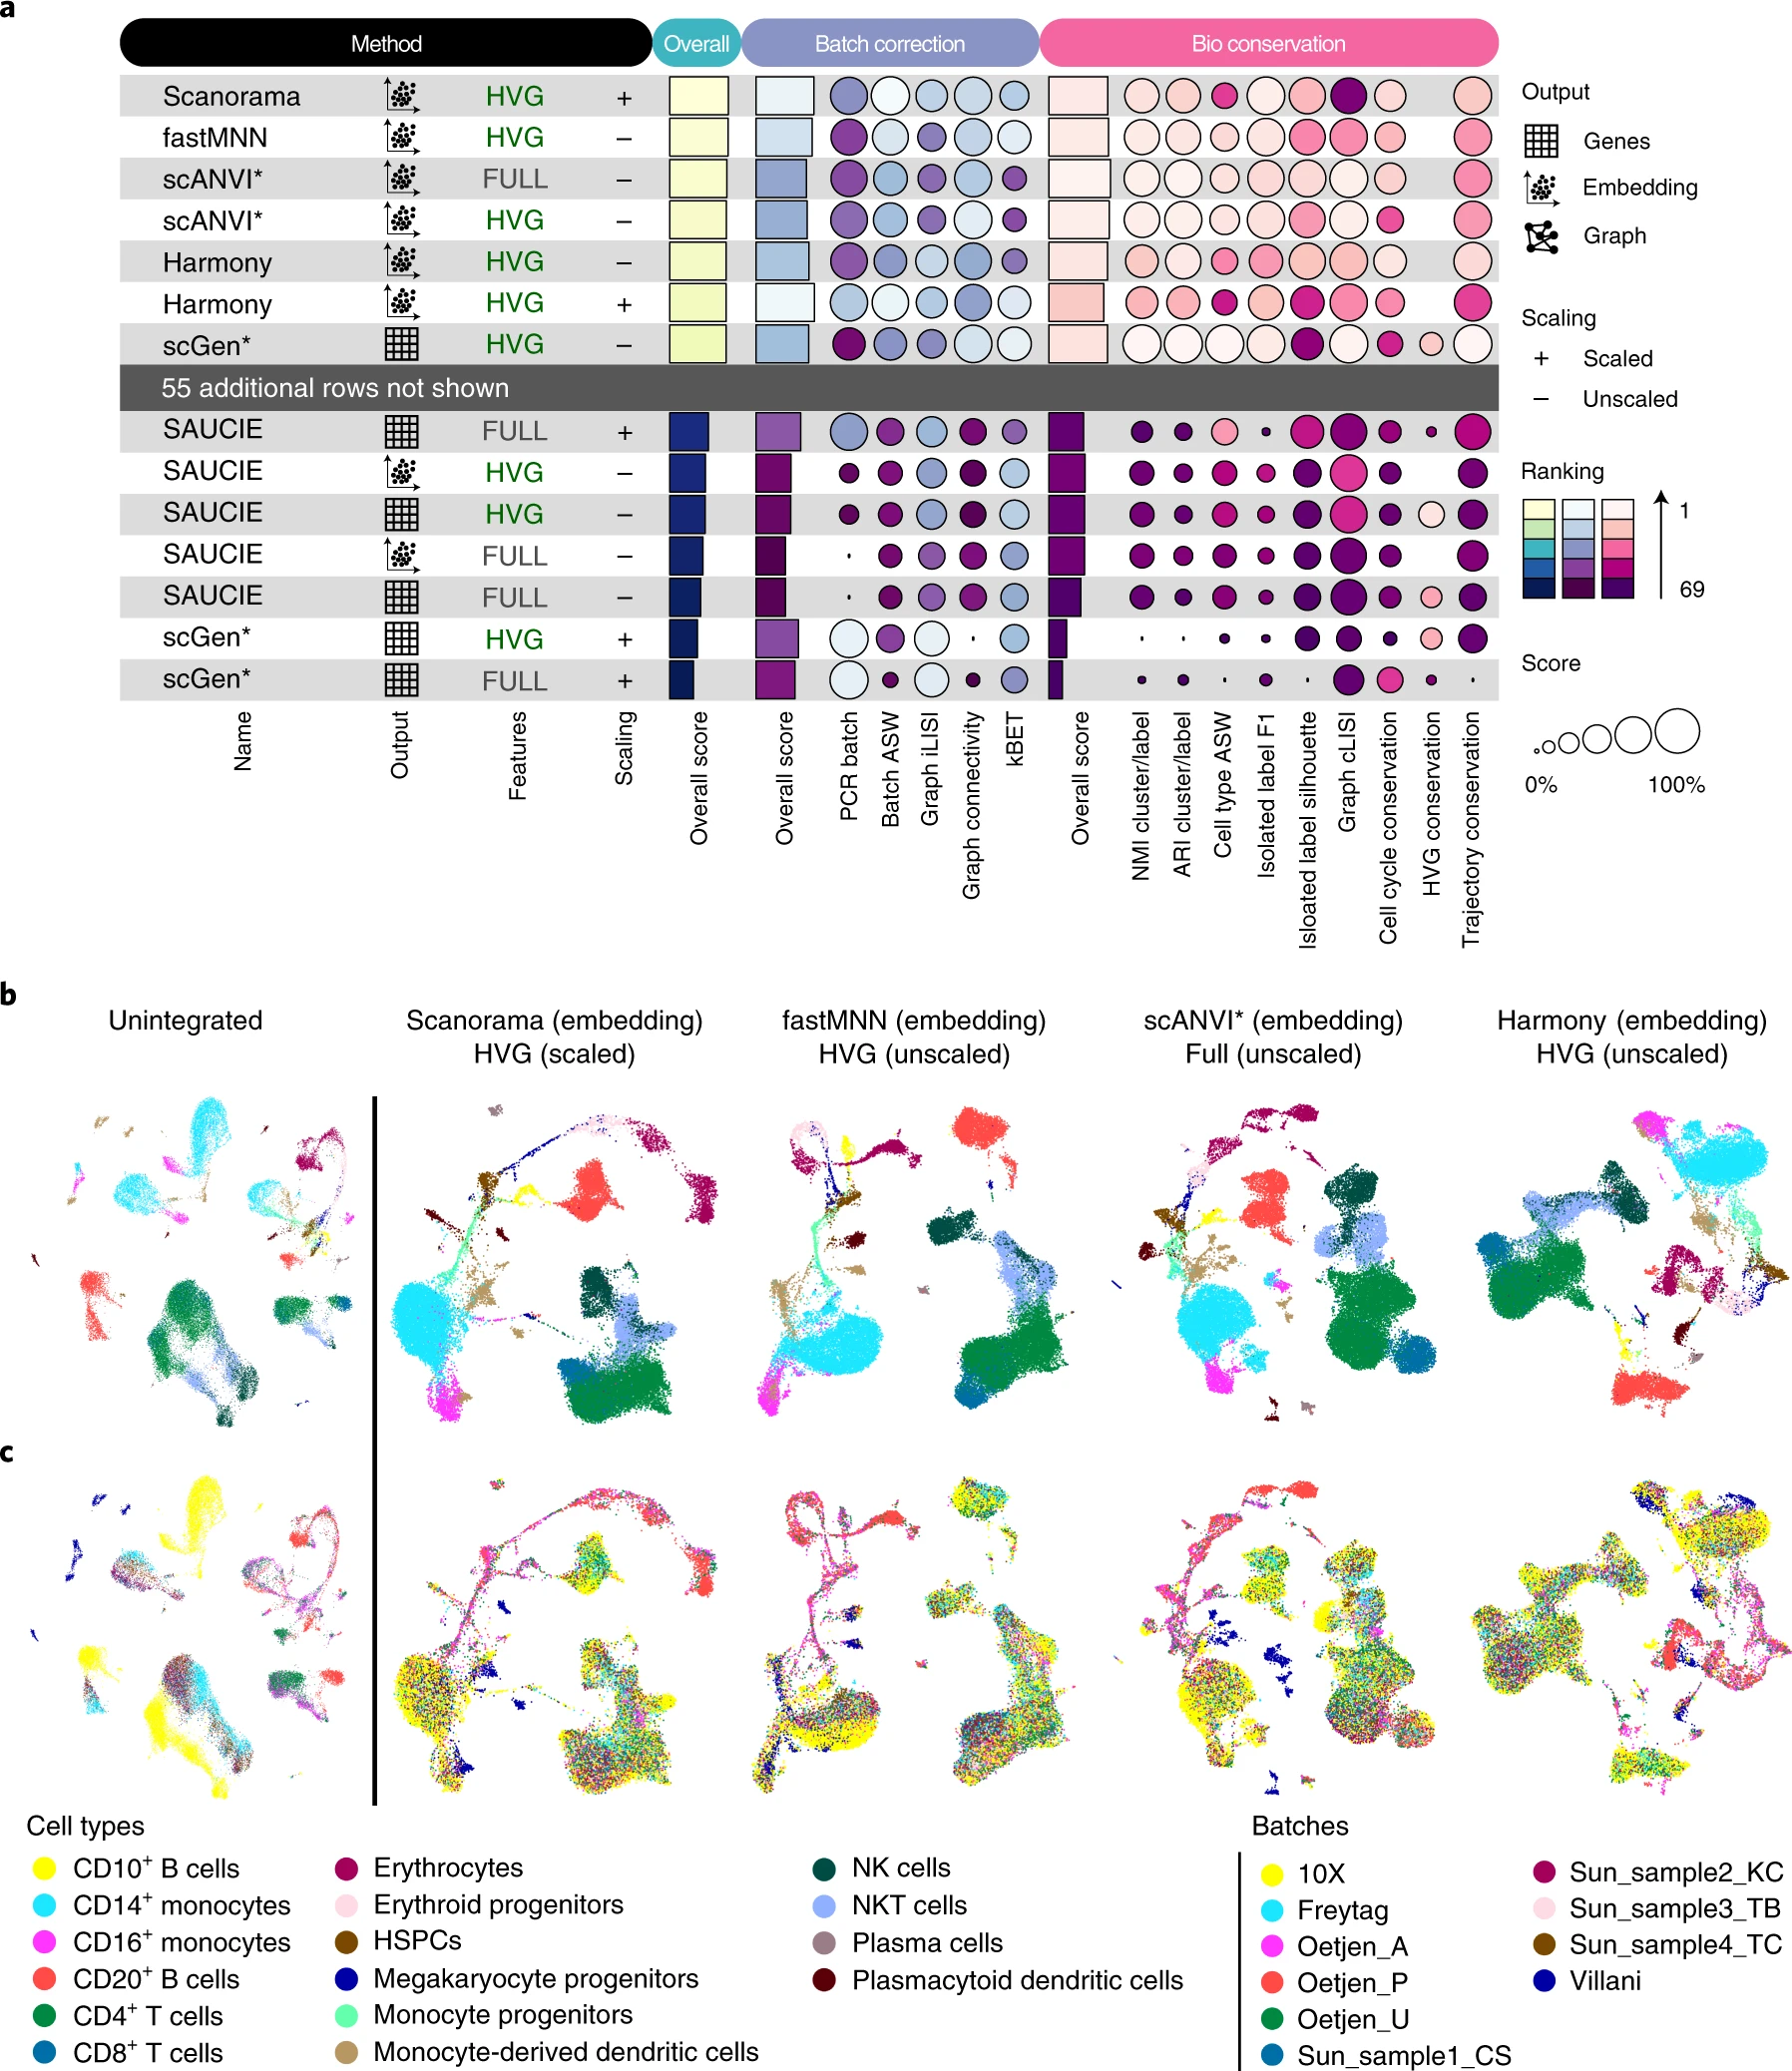
\includegraphics{./figs/singleCell/benchmarking2.jpg}
\caption{Benchmarking results for the human immune cell task.}
\end{figure}

\hypertarget{technology-related}{%
\chapter{Technology Related}\label{technology-related}}

\hypertarget{scrna-seq-modelling}{%
\section{scRNA-seq modelling}\label{scrna-seq-modelling}}

\hypertarget{nb-models-for-scrna-seq}{%
\subsection{NB models for scRNA-seq}\label{nb-models-for-scrna-seq}}

KEY WORDS: \textbf{scRNA-seq counts}

\href{http://web.stanford.edu/class/bios221/book/Chap-CountData.html}{TUTORIAL-High-Throughput Count Data}

DEseq2, scTransform, BASICS

\hypertarget{deseq2}{%
\subsubsection{DEseq2}\label{deseq2}}

\textbf{\href{https://genomebiology.biomedcentral.com/articles/10.1186/s13059-014-0550-8}{Moderated estimation of fold change and dispersion for RNA-seq data with DESeq2}\citep{love2014moderated}}

\begin{figure}
\centering
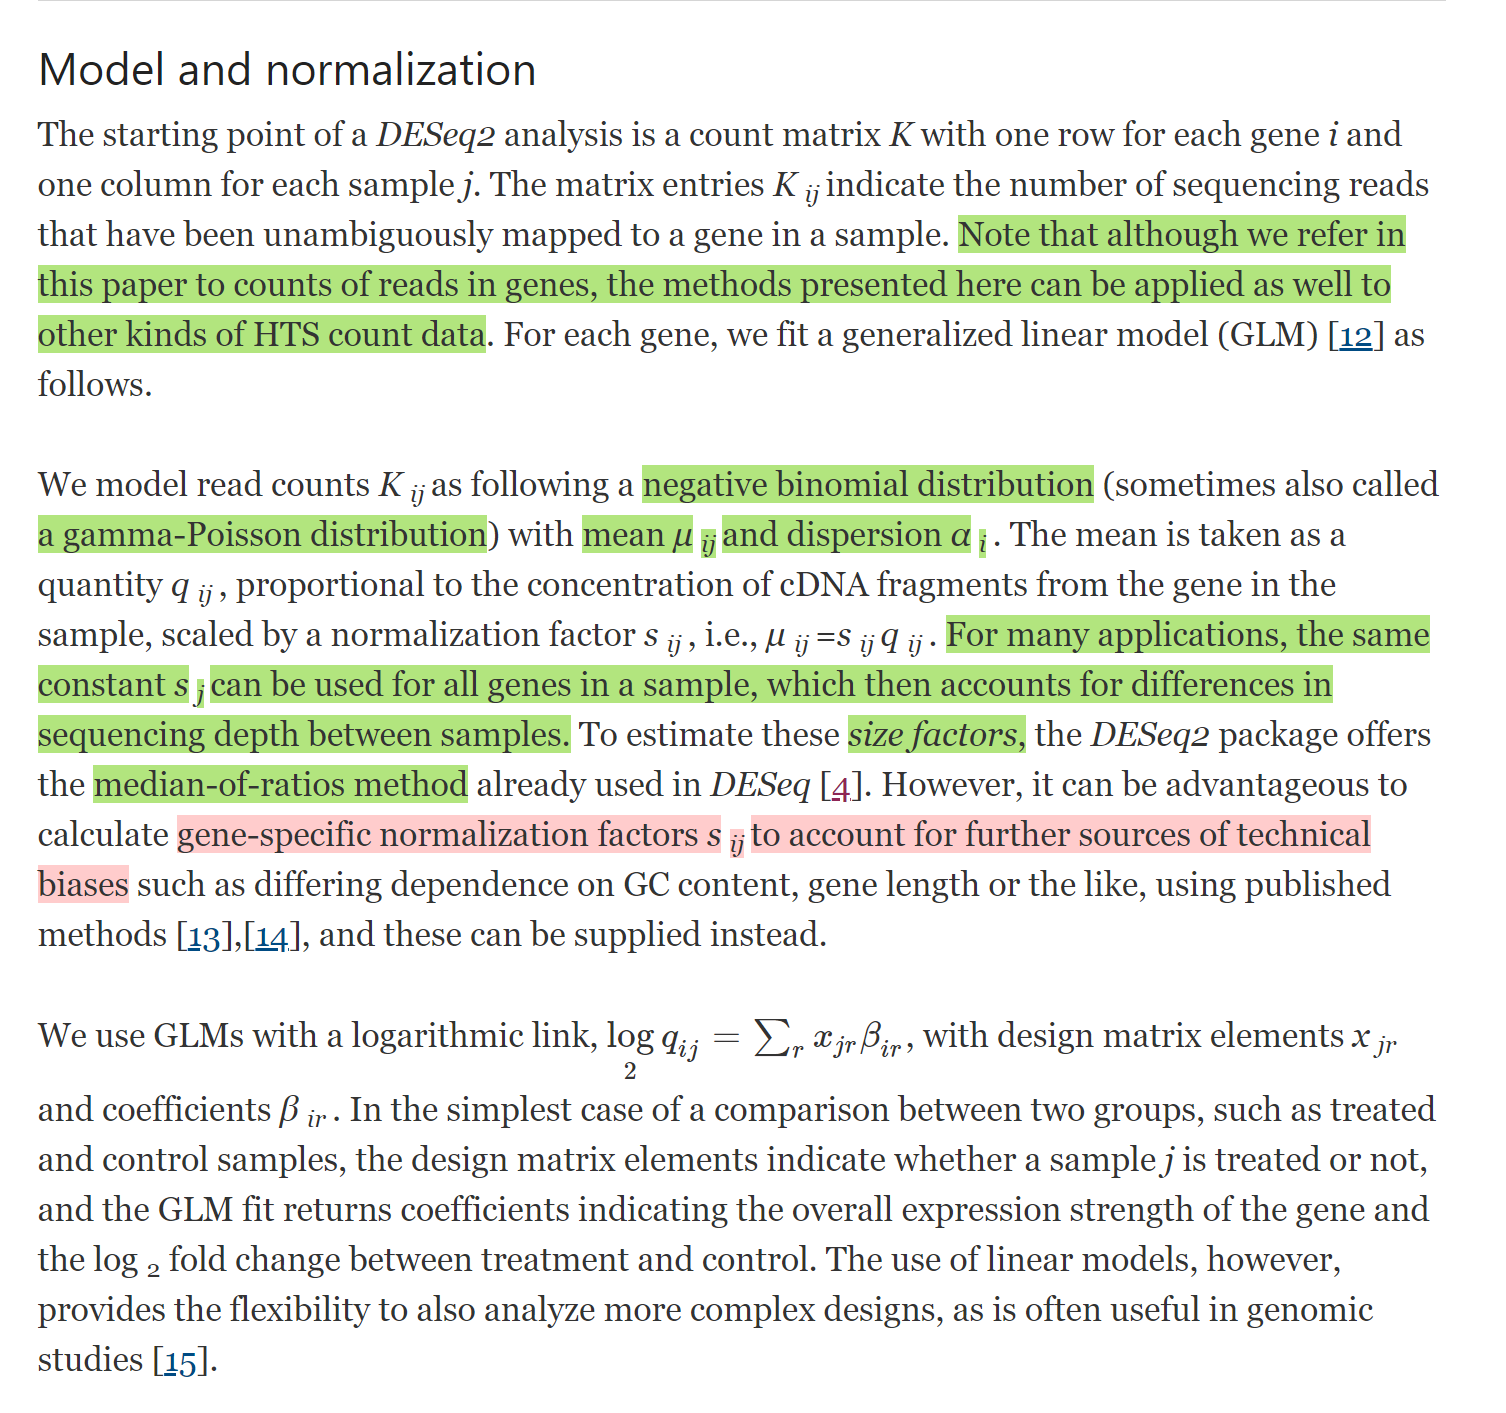
\includegraphics{./figs/RNAseqCounts/DEseq2.png}
\caption{DEseq2}
\end{figure}

\begin{figure}
\centering
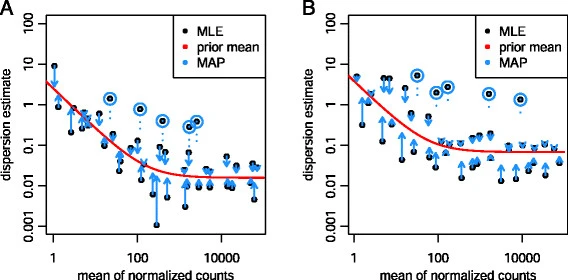
\includegraphics{./figs/RNAseqCounts/DEseq2_Fig1.png}
\caption{DEseq2-fig1}
\end{figure}

\textbf{Shrinkage estimation of dispersion.} Plot of dispersion estimates over the average expression strength (A) for the Bottomly et al.~{[}16{]} dataset with six samples across two groups and (B) for five samples from the Pickrell et al.~{[}17{]} dataset, fitting only an intercept term. First, gene-wise MLEs are obtained using only the respective genes data (black dots). Then, a curve (red) is fit to the MLEs to capture the overall trend of dispersion-mean dependence. This fit is used as a prior mean for a second estimation round, which results in the final MAP estimates of dispersion (arrow heads). This can be understood as a shrinkage (along the blue arrows) of the noisy gene-wise estimates toward the consensus represented by the red line. The black points circled in blue are detected as dispersion outliers and not shrunk toward the prior (shrinkage would follow the dotted line). For clarity, only a subset of genes is shown, which is enriched for dispersion outliers. Additional file 1: Figure S1 displays the same data but with dispersions of all genes shown. MAP, maximum a posteriori; MLE, maximum-likelihood estimate.

\hypertarget{sctransform}{%
\subsubsection{scTransform}\label{sctransform}}

\texttt{Our\ procedure\ is\ broadly\ applicable\ for\ any\ UMI-based\ scRNA-seq\ dataset\ and\ is\ freely\ available\ to\ users\ through\ the\ open-source\ R\ package\ sctransform\ (github.com/ChristophH/sctransform),\ with\ a\ direct\ interface\ to\ our\ single-cell\ toolkit\ Seurat.}

\texttt{**Pearson\ residuals**\ from\ "regularized\ negative\ binomial\ regression,"\ help\ remove\ the\ influence\ of\ technical\ characteristics\ from\ downstream\ analyses\ while\ preserving\ biological\ heterogeneity}

\texttt{unconstrained\ negative\ binomial\ model\ may\ overfit\ scRNA-seq\ data,\ and\ overcome\ this\ by\ pooling\ information\ across\ genes\ with\ similar\ abundances\ to\ obtain\ stable\ parameter\ estimates.}

\textbf{\href{https://genomebiology.biomedcentral.com/articles/10.1186/s13059-019-1874-1}{Normalization and variance stabilization of single-cell RNA-seq data using regularized negative binomial regression}\citep{hafemeister2019normalization}}

\url{https://github.com/ChristophH/sctransform/}

\begin{figure}
\centering
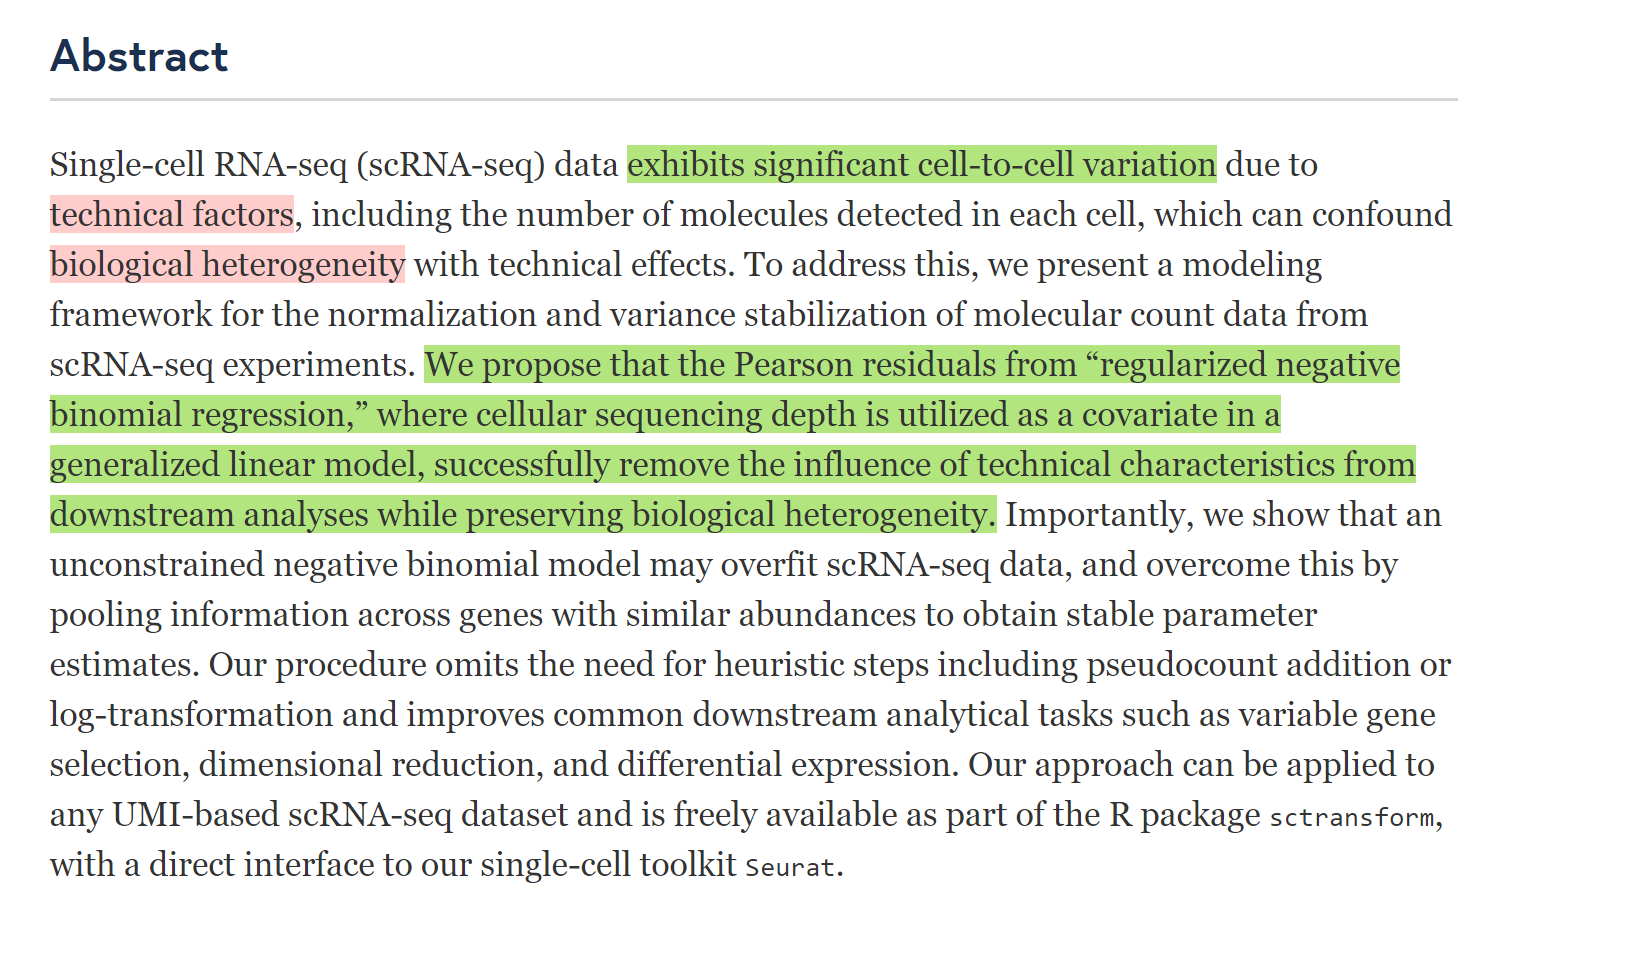
\includegraphics{./figs/RNAseqCounts/sctransform.png}
\caption{SCTransform}
\end{figure}

We propose that the Pearson residuals from regularized negative binomial regression, where cellular sequencing depth is utilized as a covariate in a generalized linear model, successfully remove the influence of technical characteristics from downstream analyses while preserving biological heterogeneity.

\begin{itemize}
\tightlist
\item
  UMI-based scRNA-seq dataset
\end{itemize}

\begin{figure}
\centering
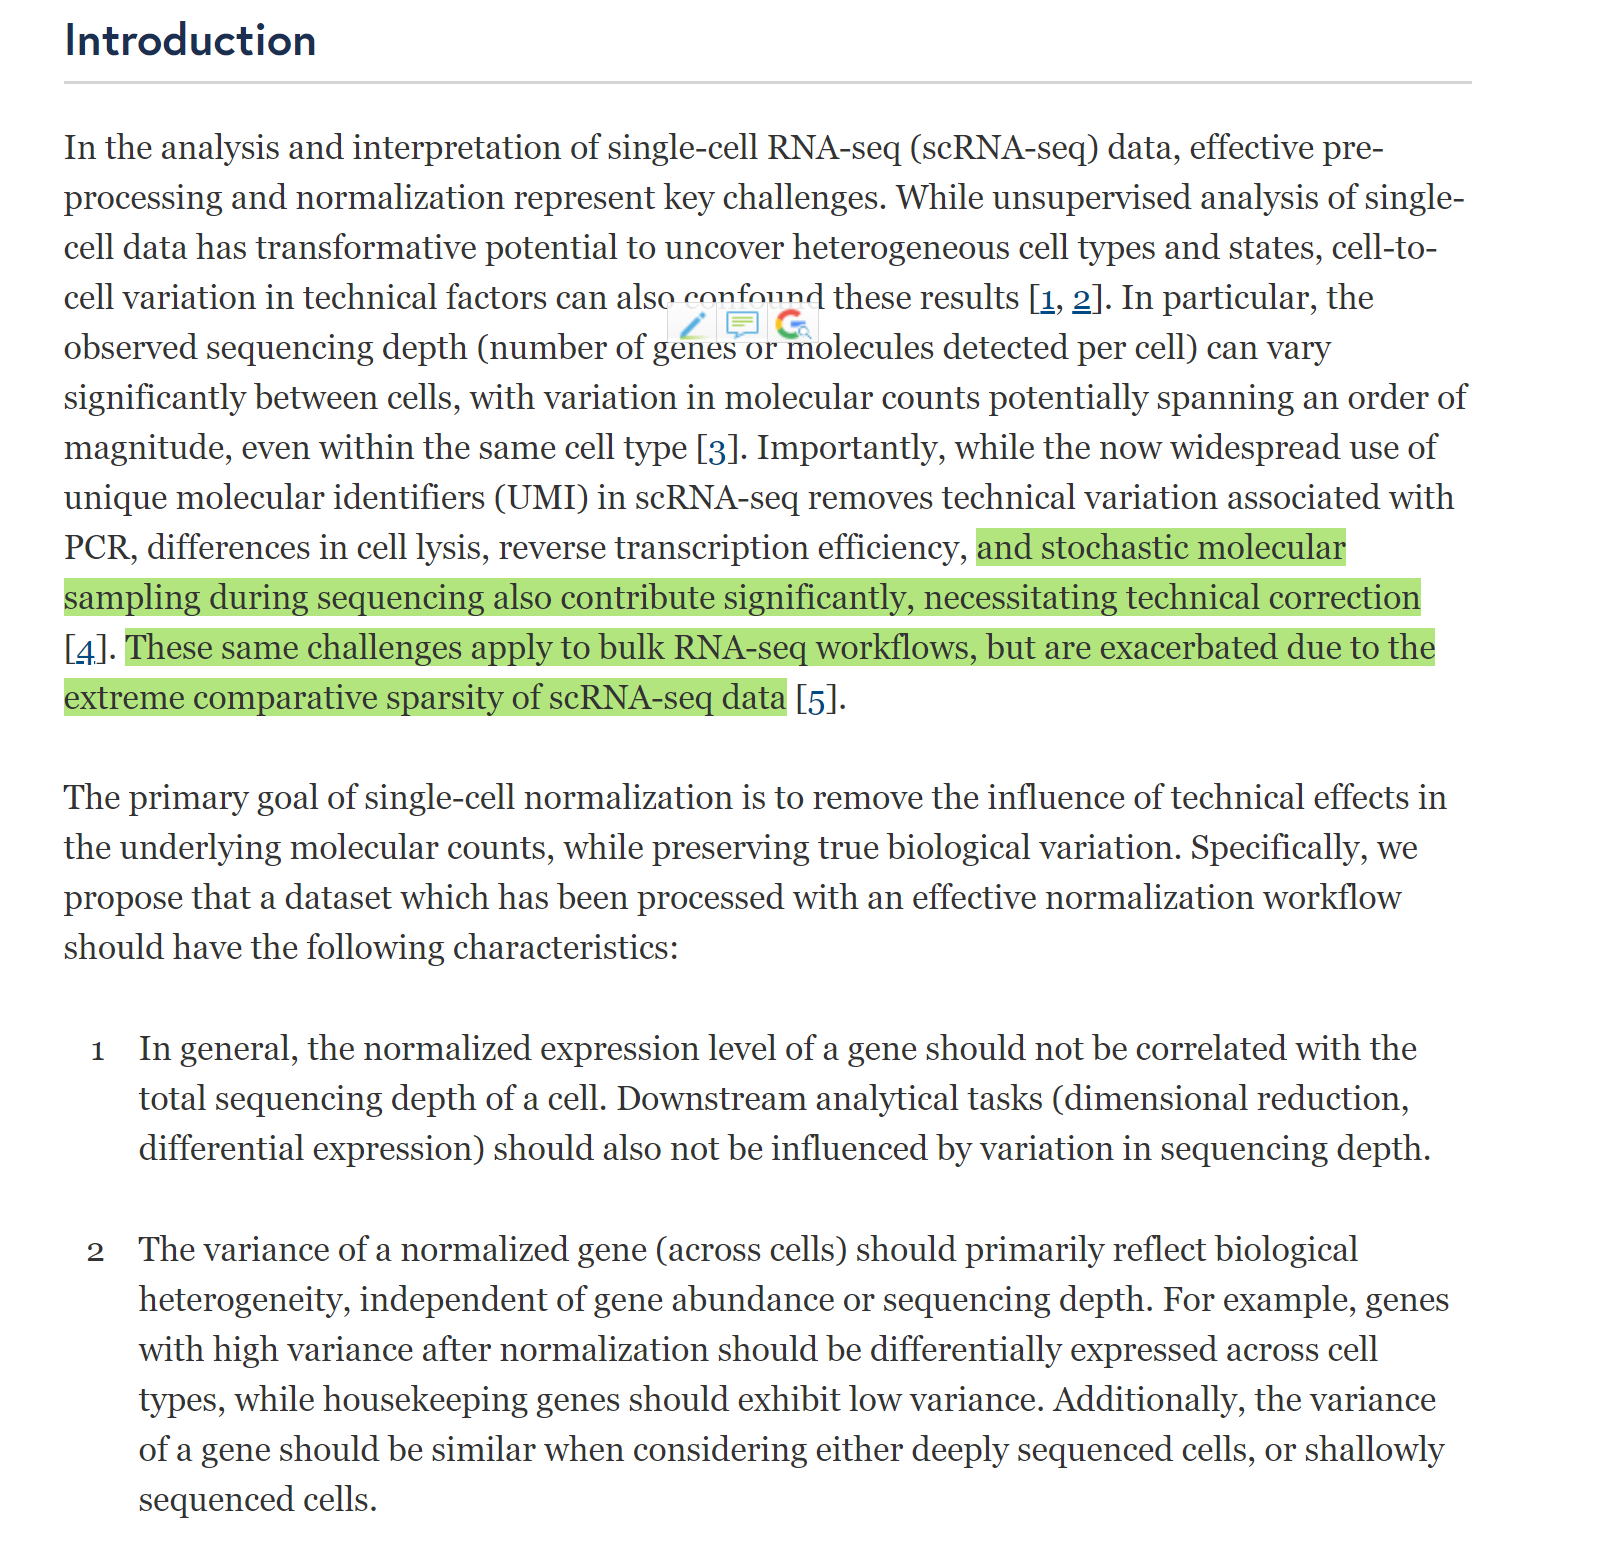
\includegraphics{./figs/RNAseqCounts/sctransform-intro.png}
\caption{SCTransform-intro}
\end{figure}

\texttt{observed\ **sequencing\ depth**\ (number\ of\ genes\ or\ molecules\ detected\ per\ cell)\ can\ vary\ significantly\ between\ cells,\ with\ variation\ in\ molecular\ counts\ potentially\ spanning\ an\ order\ of\ magnitude,\ even\ within\ the\ same\ cell\ type}

\texttt{while\ the\ now\ widespread\ use\ of\ unique\ molecular\ identifiers\ (UMI)\ in\ scRNA-seq\ removes\ technical\ variation\ associated\ with\ PCR,\ differences\ in\ cell\ lysis,\ reverse\ transcription\ efficiency,\ and\ stochastic\ molecular\ sampling\ during\ sequencing\ also\ contribute\ significantly,\ necessitating\ technical\ correction}

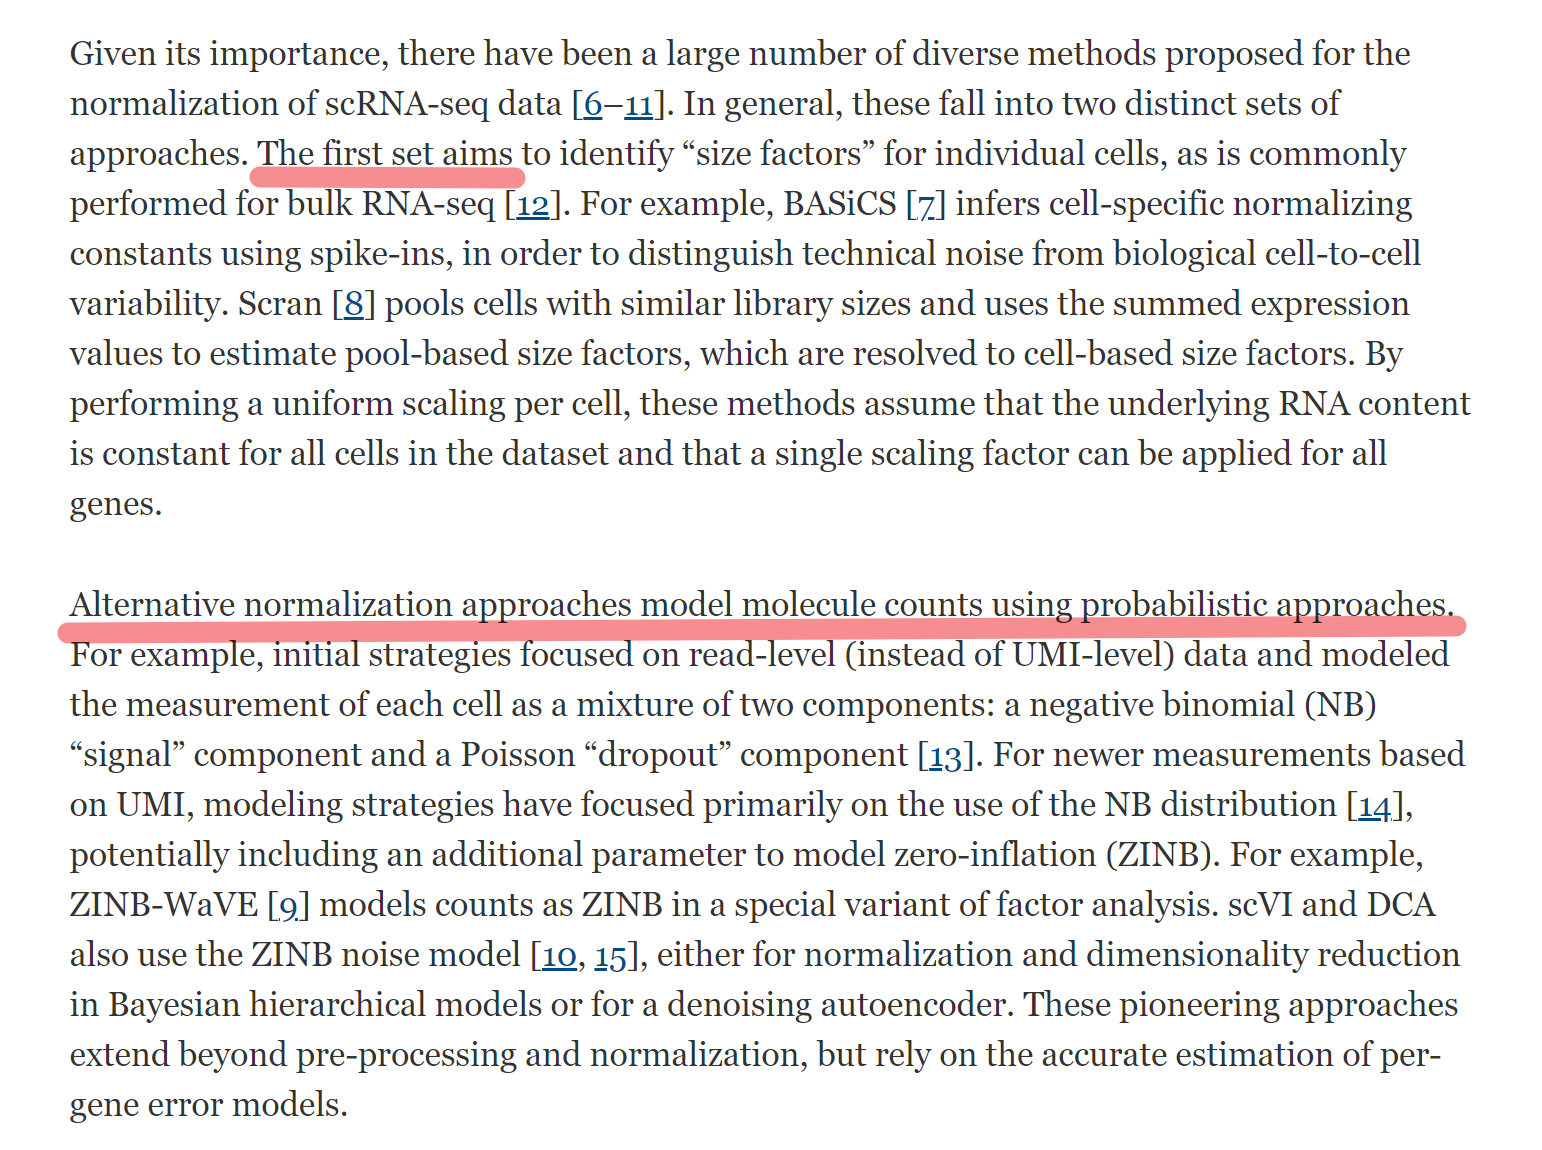
\includegraphics{./figs/RNAseqCounts/background.png}
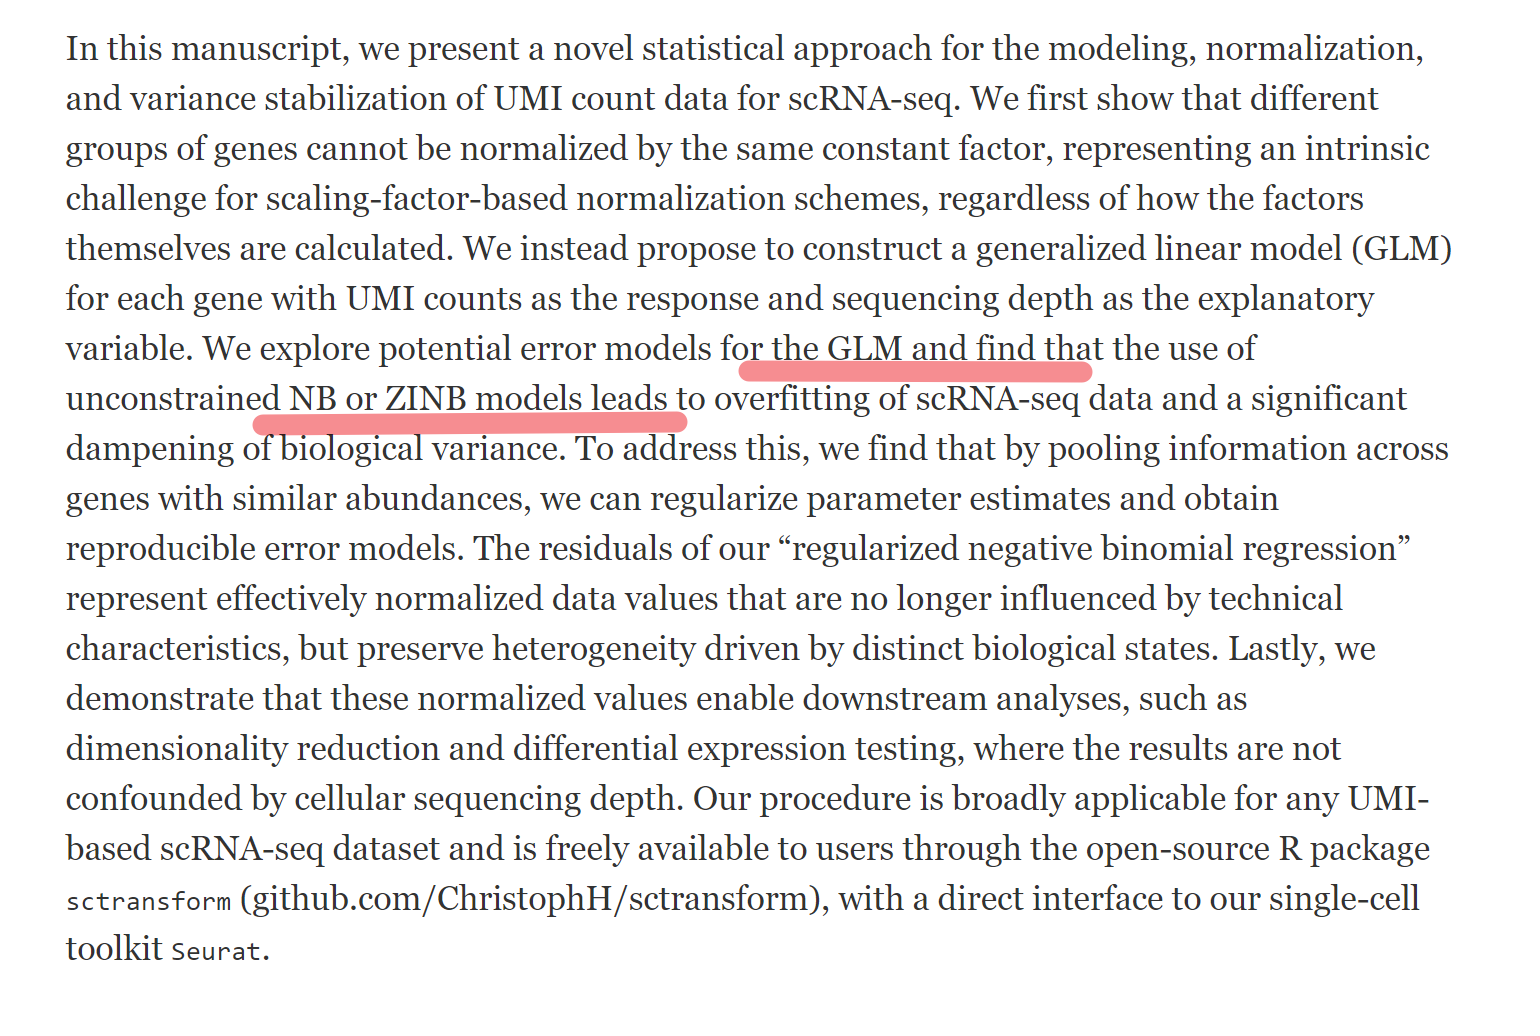
\includegraphics{./figs/RNAseqCounts/sctrans_intro.png}
\textbf{Results}

\begin{itemize}
\item
  A single scaling factor does not effectively normalize both lowly and highly expressed genes
\item
  Modeling single-cell data with a negative binomial distribution leads to overfitting
\item
  Applying regularized negative binomial regression for single-cell normalization
\item
  Pearson residuals effectively normalize technical differences, while retaining biological variation
\item
  Downstream analytical tasks are not biased by sequencing depth
\end{itemize}

\begin{figure}
\centering
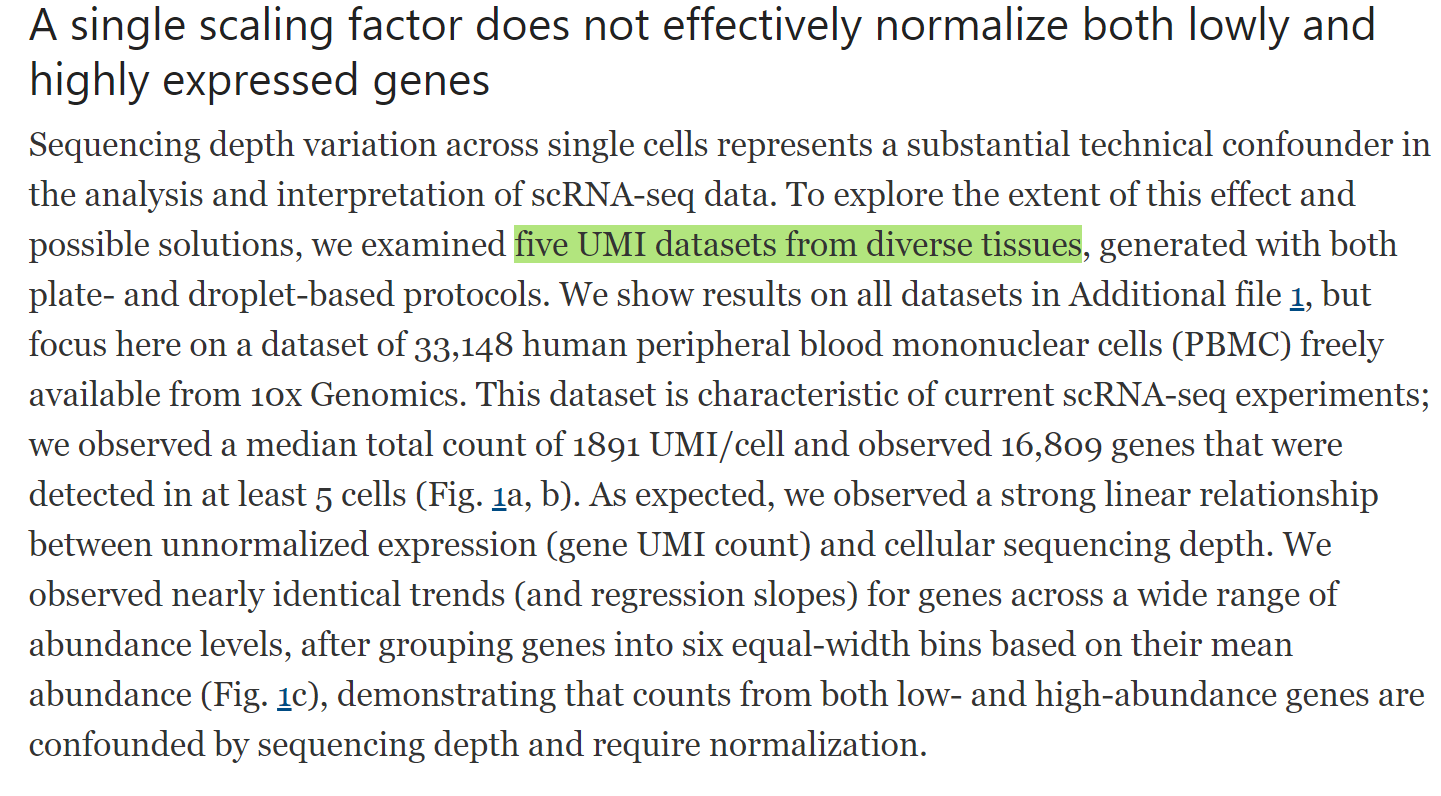
\includegraphics{./figs/RNAseqCounts/sctransform-sequencing depth.png}
\caption{.}
\end{figure}

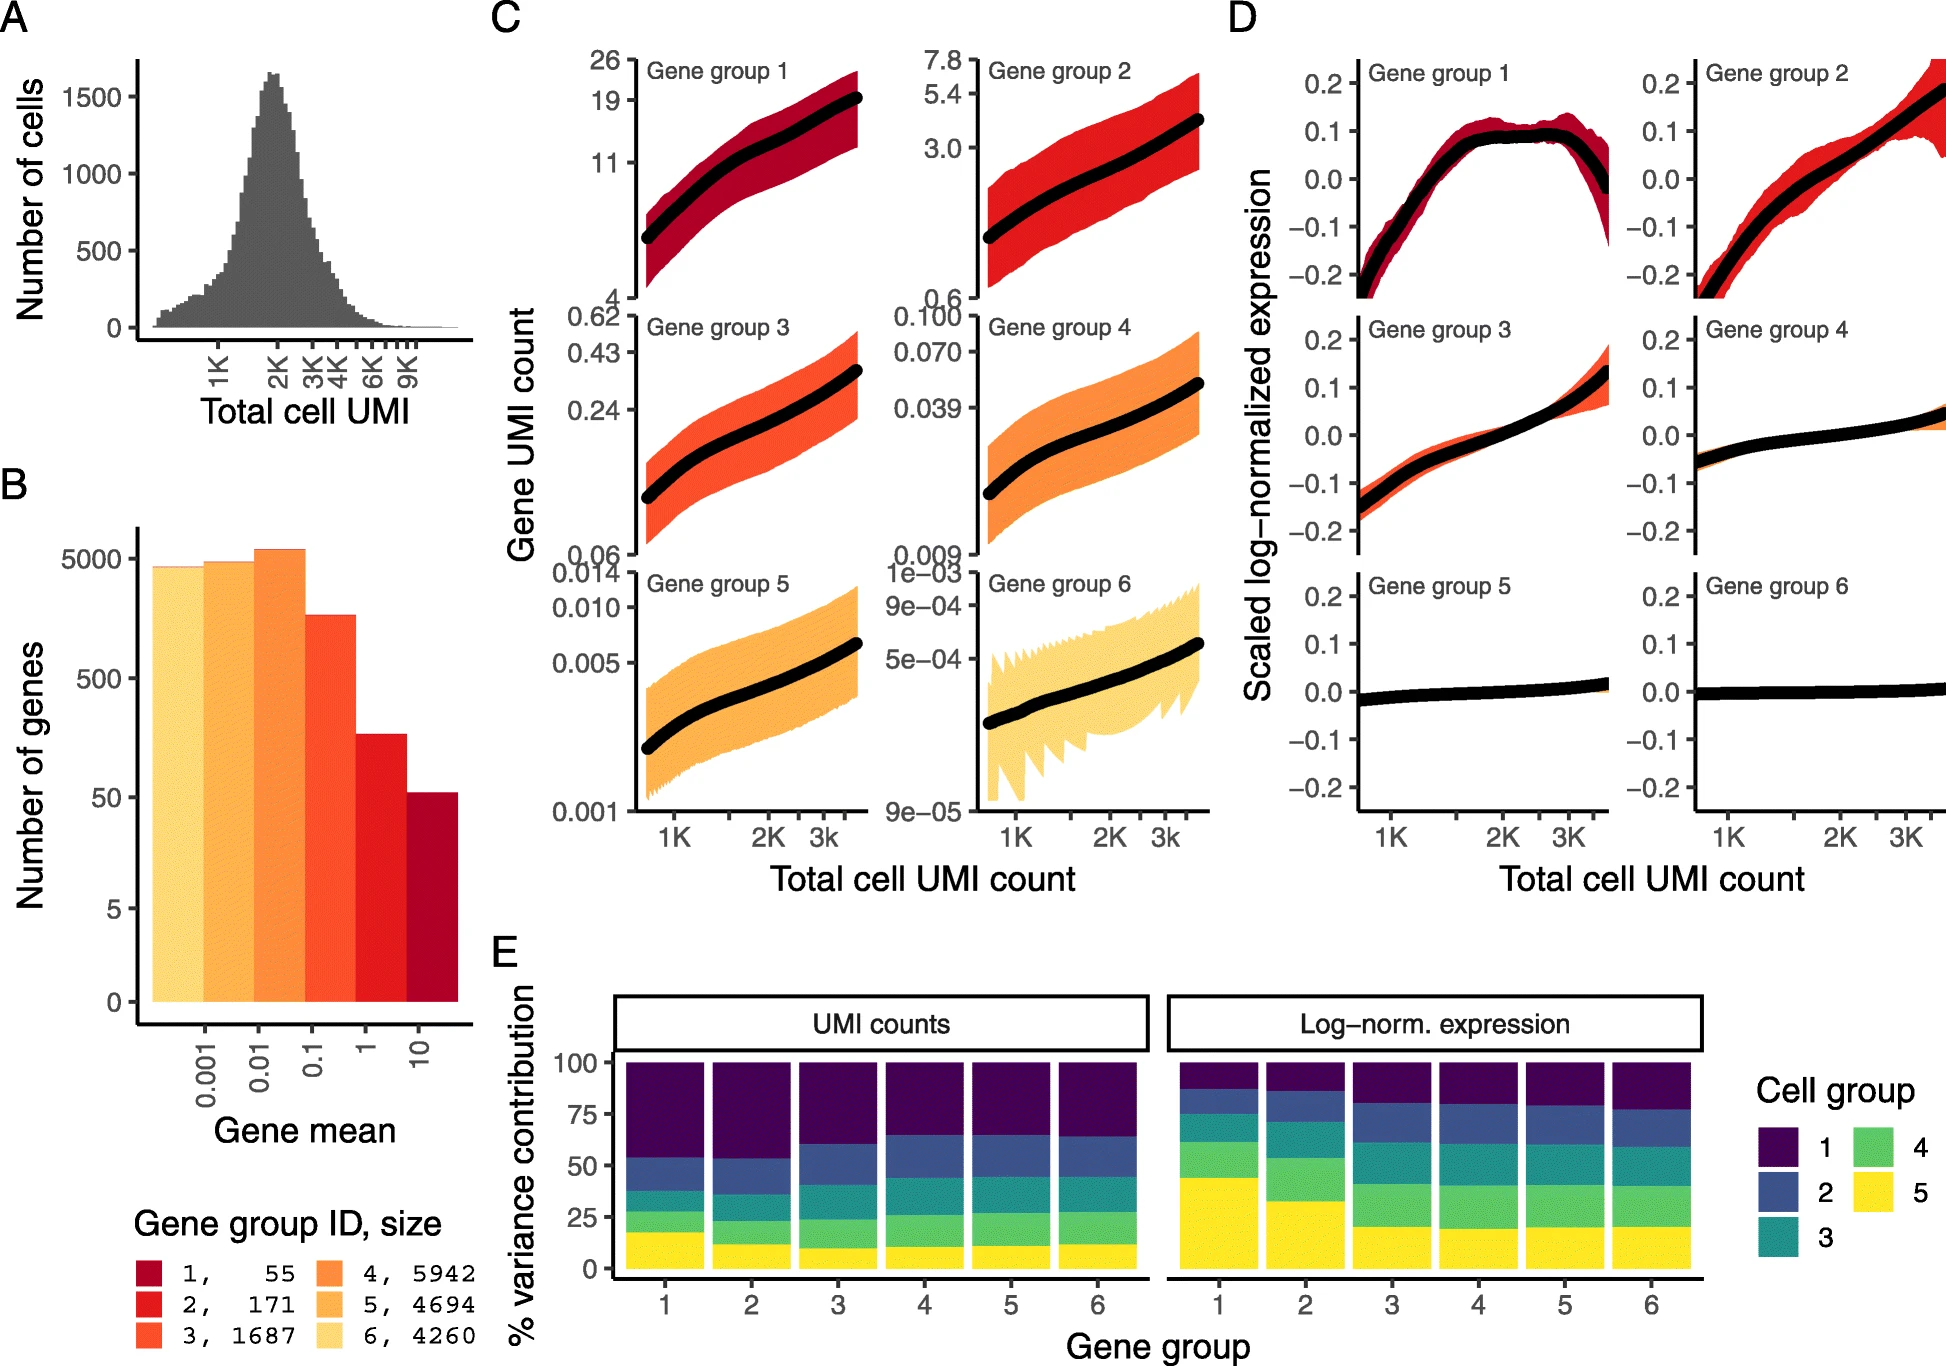
\includegraphics{./figs/RNAseqCounts/sctransform-fig1.png}
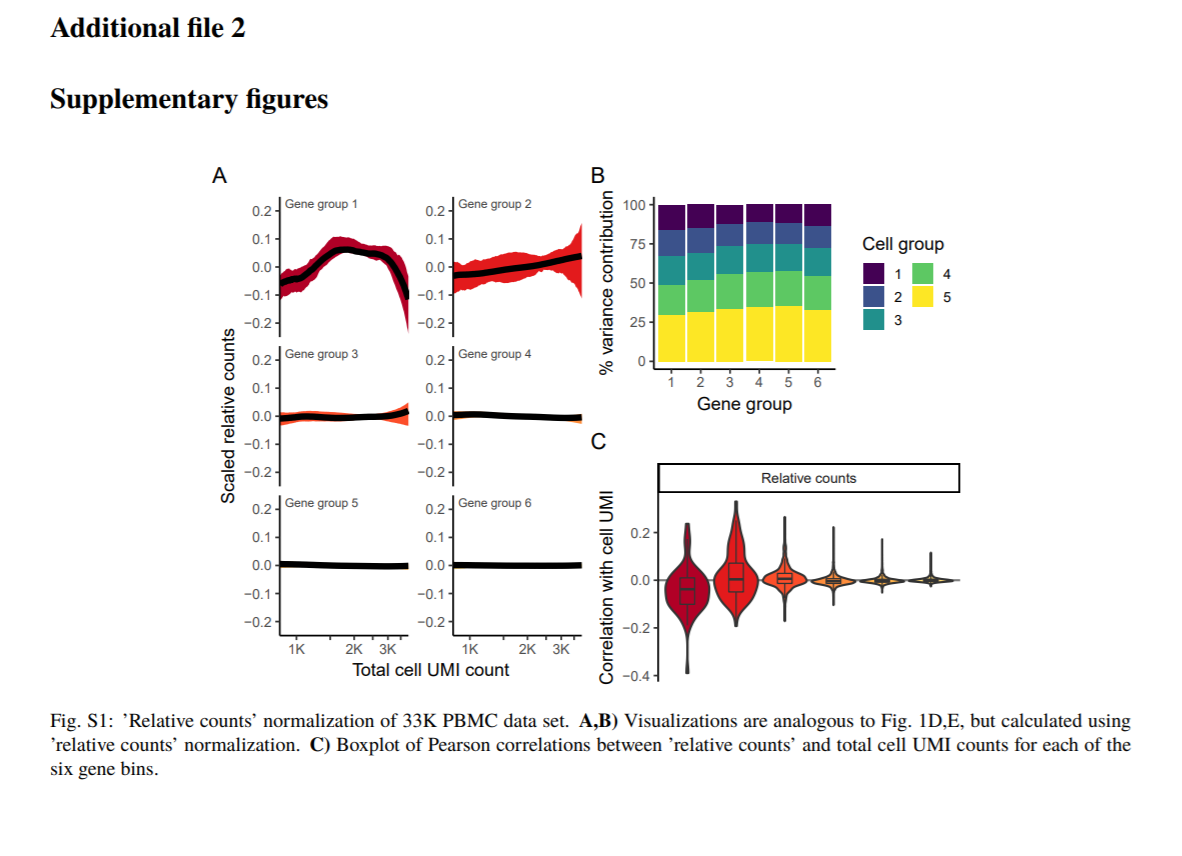
\includegraphics{./figs/RNAseqCounts/sctransform-figS1.png}

\textbf{Methods}

\begin{itemize}
\tightlist
\item
  Regularized negative binomial regression
\end{itemize}

\hypertarget{basics}{%
\subsubsection{BASiCS}\label{basics}}

\textbf{\href{https://journals.plos.org/ploscompbiol/article?id=10.1371/journal.pcbi.1004333}{BASiCS: Bayesian Analysis of Single-Cell Sequencing Data}\citep{vallejos2015basics}}

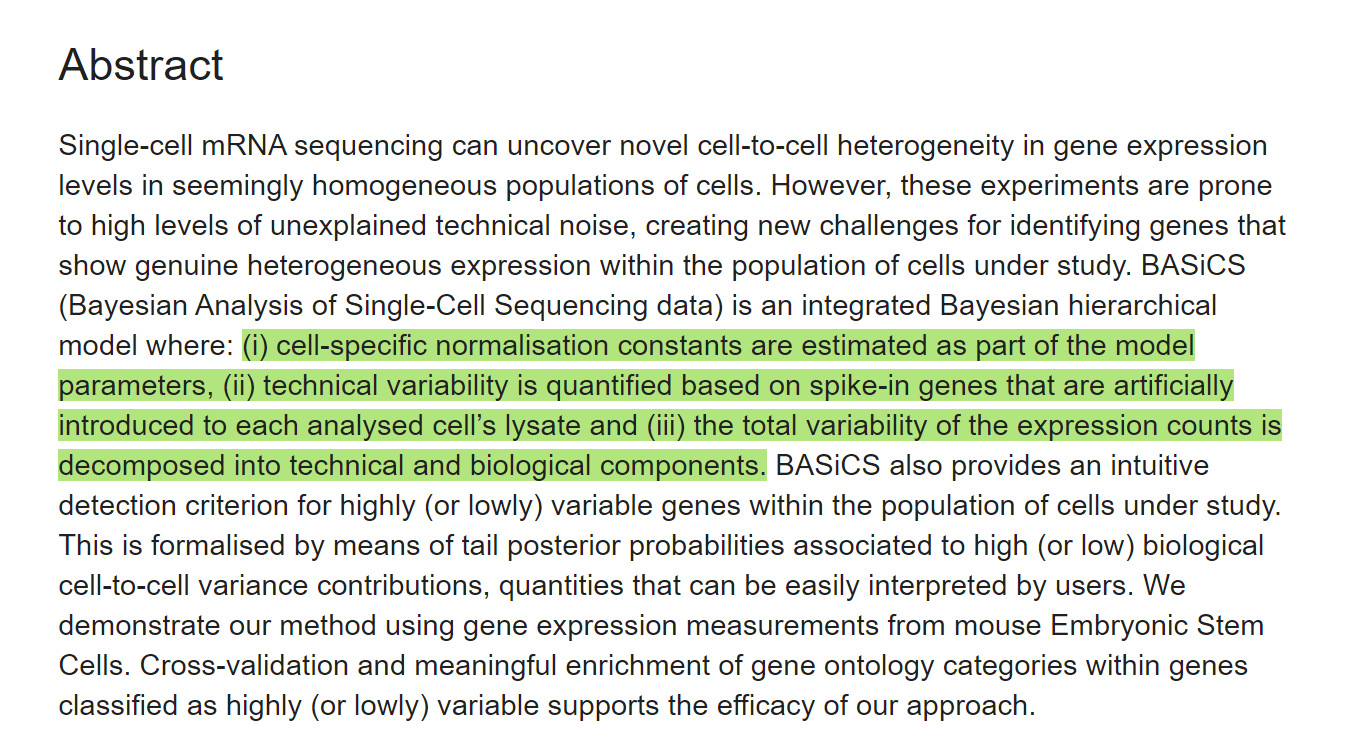
\includegraphics{./figs/RNAseqCounts/BASICS.png}
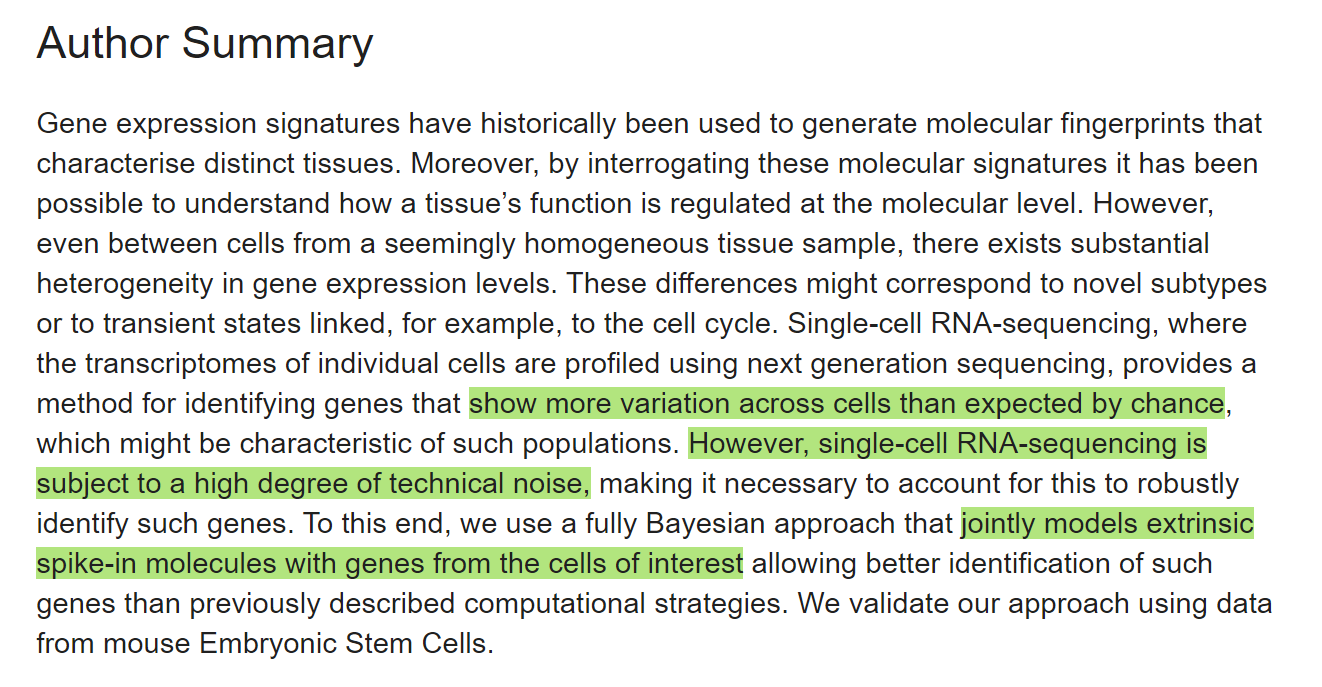
\includegraphics{./figs/RNAseqCounts/BASICS2.png}
\textbf{INTRODUCTION}

\begin{itemize}
\tightlist
\item
  Cell\_SPECIFIC NORMALIZATION
\end{itemize}

For instance, in Fig 1(a), each gene has the same expression rate in both cells, yet the expression counts in the first cell will be roughly twice as much as those from the second cell. In the same spirit, if different sequencing depths (the number of times a single nucleotide is read during the sequencing) are applied to these cells, the scale of expression counts will also be affected. Thus, normalisation is a crucial issue in this context.

\begin{itemize}
\tightlist
\item
  gene specific variation
\end{itemize}

Another fundamental problem for interpreting single-cell sequencing is the presence of high levels of unexplained technical noise (unrelated to sequencing depth and other amplification biases) {[}5{]}. This creates new challenges for identifying genes that show genuine biological cell-to-cell heterogeneity-beyond that induced by technical variation-and motivates the systematic inclusion of spike-in genes in single-cell experiments

\begin{itemize}
\tightlist
\item
  UMI
\end{itemize}

Recently, the introduction of Unique Molecular Identifiers (UMI) attached to each cDNA molecule during reverse transcription has substantially reduced the levels of unexplained technical noise and eliminated the effect of sequencing depth changes and other amplification biases in single-cell experiments.

Nevertheless, our analysis of a mouse Embryonic Stem Cells (ESC) suggests that unexplained technical variability can not be completely removed by using UMIs (see Results section) and that an accurate quantification of technical variability still remains important.

\textbf{HIGHLIGHT}

In BASiCS (Bayesian Analysis of Single-Cell Sequencing data), a joint model of biological and spike-in genes is formulated to simultaneously quantify unexplained technical noise and cell-to-cell biological heterogeneity using the complete set of data, borrowing information between both sets of genes (spike-in and biological) through common parameters in a hierarchical structure. Additionally, BASiCS incorporates an automated normalisation method, where normalising constants are treated as model parameters.

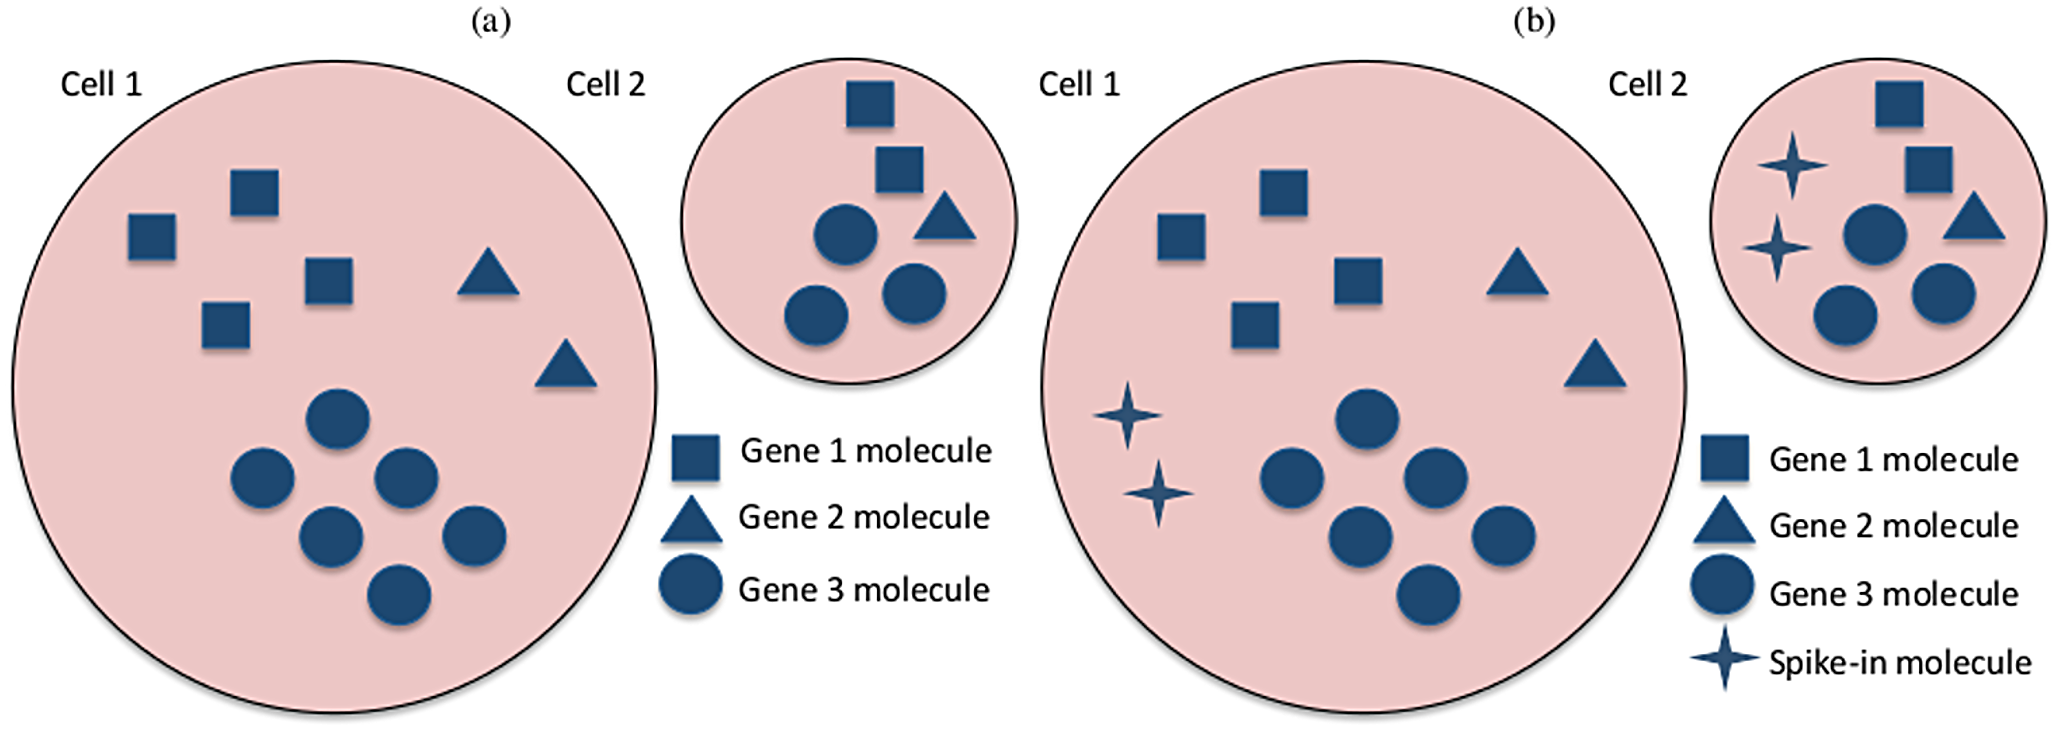
\includegraphics{./figs/RNAseqCounts/pcbi.1004333.g001.png}
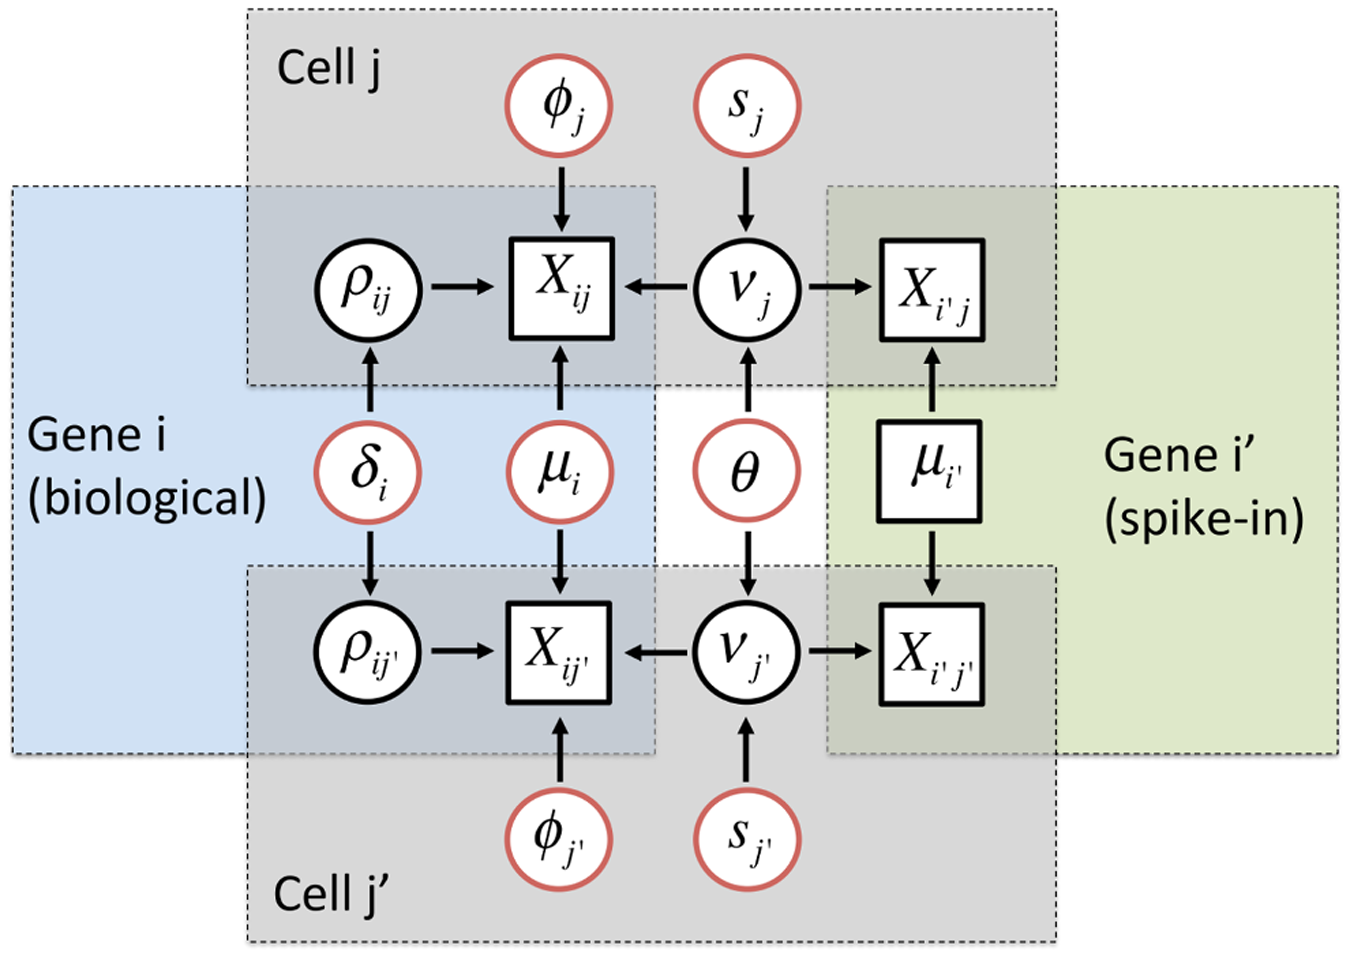
\includegraphics{./figs/RNAseqCounts/pcbi.1004333.g002.png}
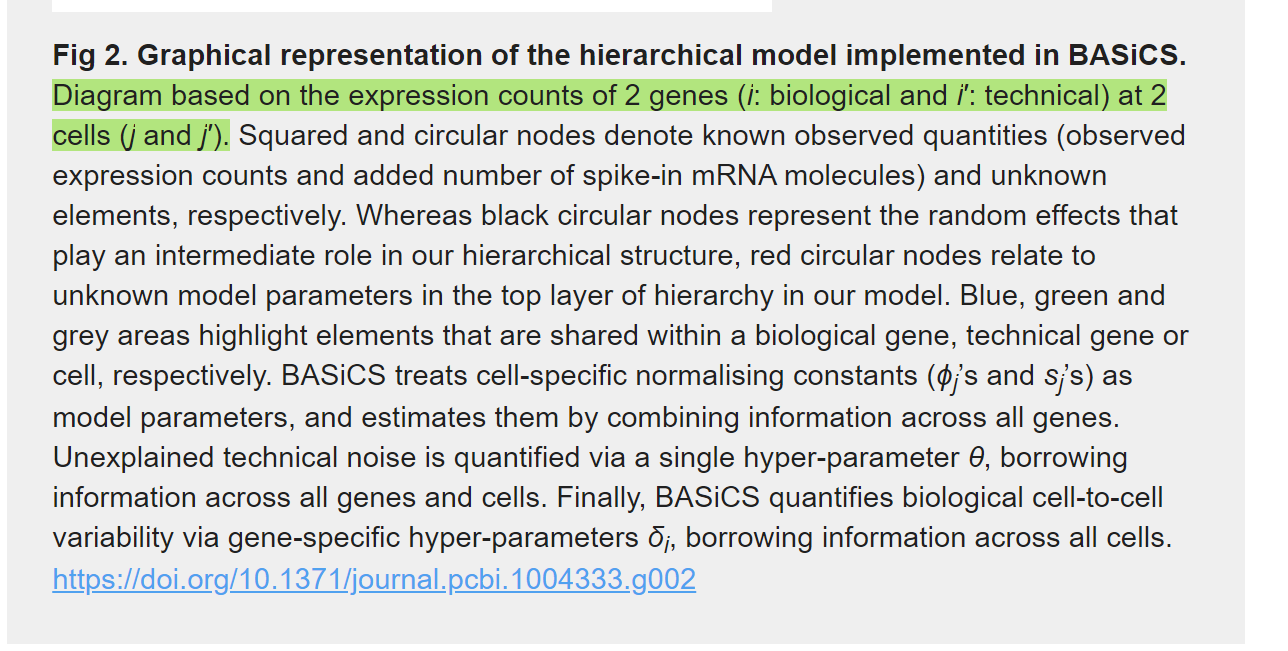
\includegraphics{./figs/RNAseqCounts/BASiCS-FIG2.png}
\#\#\#\# edgeR

\textbf{\href{https://www.ncbi.nlm.nih.gov/pmc/articles/PMC2796818/}{edgeR: a Bioconductor package for differential expression analysis of digital gene expression data}\citep{robinson2010edger}}

\textbf{\href{https://www.ncbi.nlm.nih.gov/pmc/articles/PMC3378882/}{Differential expression analysis of multifactor RNA-Seq experiments with respect to biological variation}\citep{mccarthy2012differential}}

\hypertarget{sanity}{%
\subsubsection{Sanity}\label{sanity}}

\textbf{\href{https://www.nature.com/articles/s41587-021-00875-x}{Bayesian inference of gene expression states from single-cell RNA-seq data}\citep{breda2021bayesian}}

\hypertarget{batch-effect-correction-methods-for-scrna-seq}{%
\subsection{Batch-effect correction methods for scRNA-seq}\label{batch-effect-correction-methods-for-scrna-seq}}

\textbf{\href{https://link.springer.com/article/10.1186/s13059-019-1850-9}{A benchmark of batch-effect correction methods for single-cell RNA sequencing data}\citep{tran2020benchmark}}

\begin{itemize}
\tightlist
\item
  Abstract
  \textbf{Background}: Large-scale single-cell transcriptomic datasets generated using different technologies contain batchspecific
  systematic variations that present a challenge to batch-effect removal and data integration. With continued
  growth expected in scRNA-seq data, achieving effective batch integration with available computational resources is
  crucial. Here, we perform an in-depth benchmark study on available batch correction methods to determine the
  most suitable method for batch-effect removal.
\end{itemize}

\textbf{Results}: We compare 14 methods in terms of computational runtime, the ability to handle large datasets, and
batch-effect correction efficacy while preserving cell type purity. Five scenarios are designed for the study: identical
cell types with different technologies, non-identical cell types, multiple batches, big data, and simulated data.
Performance is evaluated using four benchmarking metrics including kBET, LISI, ASW, and ARI. We also investigate
the use of batch-corrected data to study differential gene expression.

\textbf{Conclusion}: Based on our results, Harmony, LIGER, and Seurat 3 are the recommended methods for batch
integration. Due to its significantly shorter runtime, Harmony is recommended as the first method to try, with the
other methods as viable alternatives.

\textbf{Keywords}: Single-cell RNA-seq, Batch correction, Batch effect, Integration, Differential gene expression

\hypertarget{hi-seq}{%
\section{Hi-Seq}\label{hi-seq}}

\textbf{\href{https://www.nature.com/articles/s41587-021-00981-w}{Enhanced detection of minimal residual disease by targeted sequencing of phased variants in circulating tumor DNA}\citep{Kurtz2021}}

KEY WORDS: \textbf{phased variants}

\hypertarget{languages-and-compilers}{%
\section{languages and compilers}\label{languages-and-compilers}}

\begin{itemize}
\tightlist
\item
  Seq
\end{itemize}

\href{https://www.nature.com/articles/s41587-021-00985-6}{A Python-based programming language for high-performance computational genomics}\citep{shajii2021python}

\begin{figure}
\centering
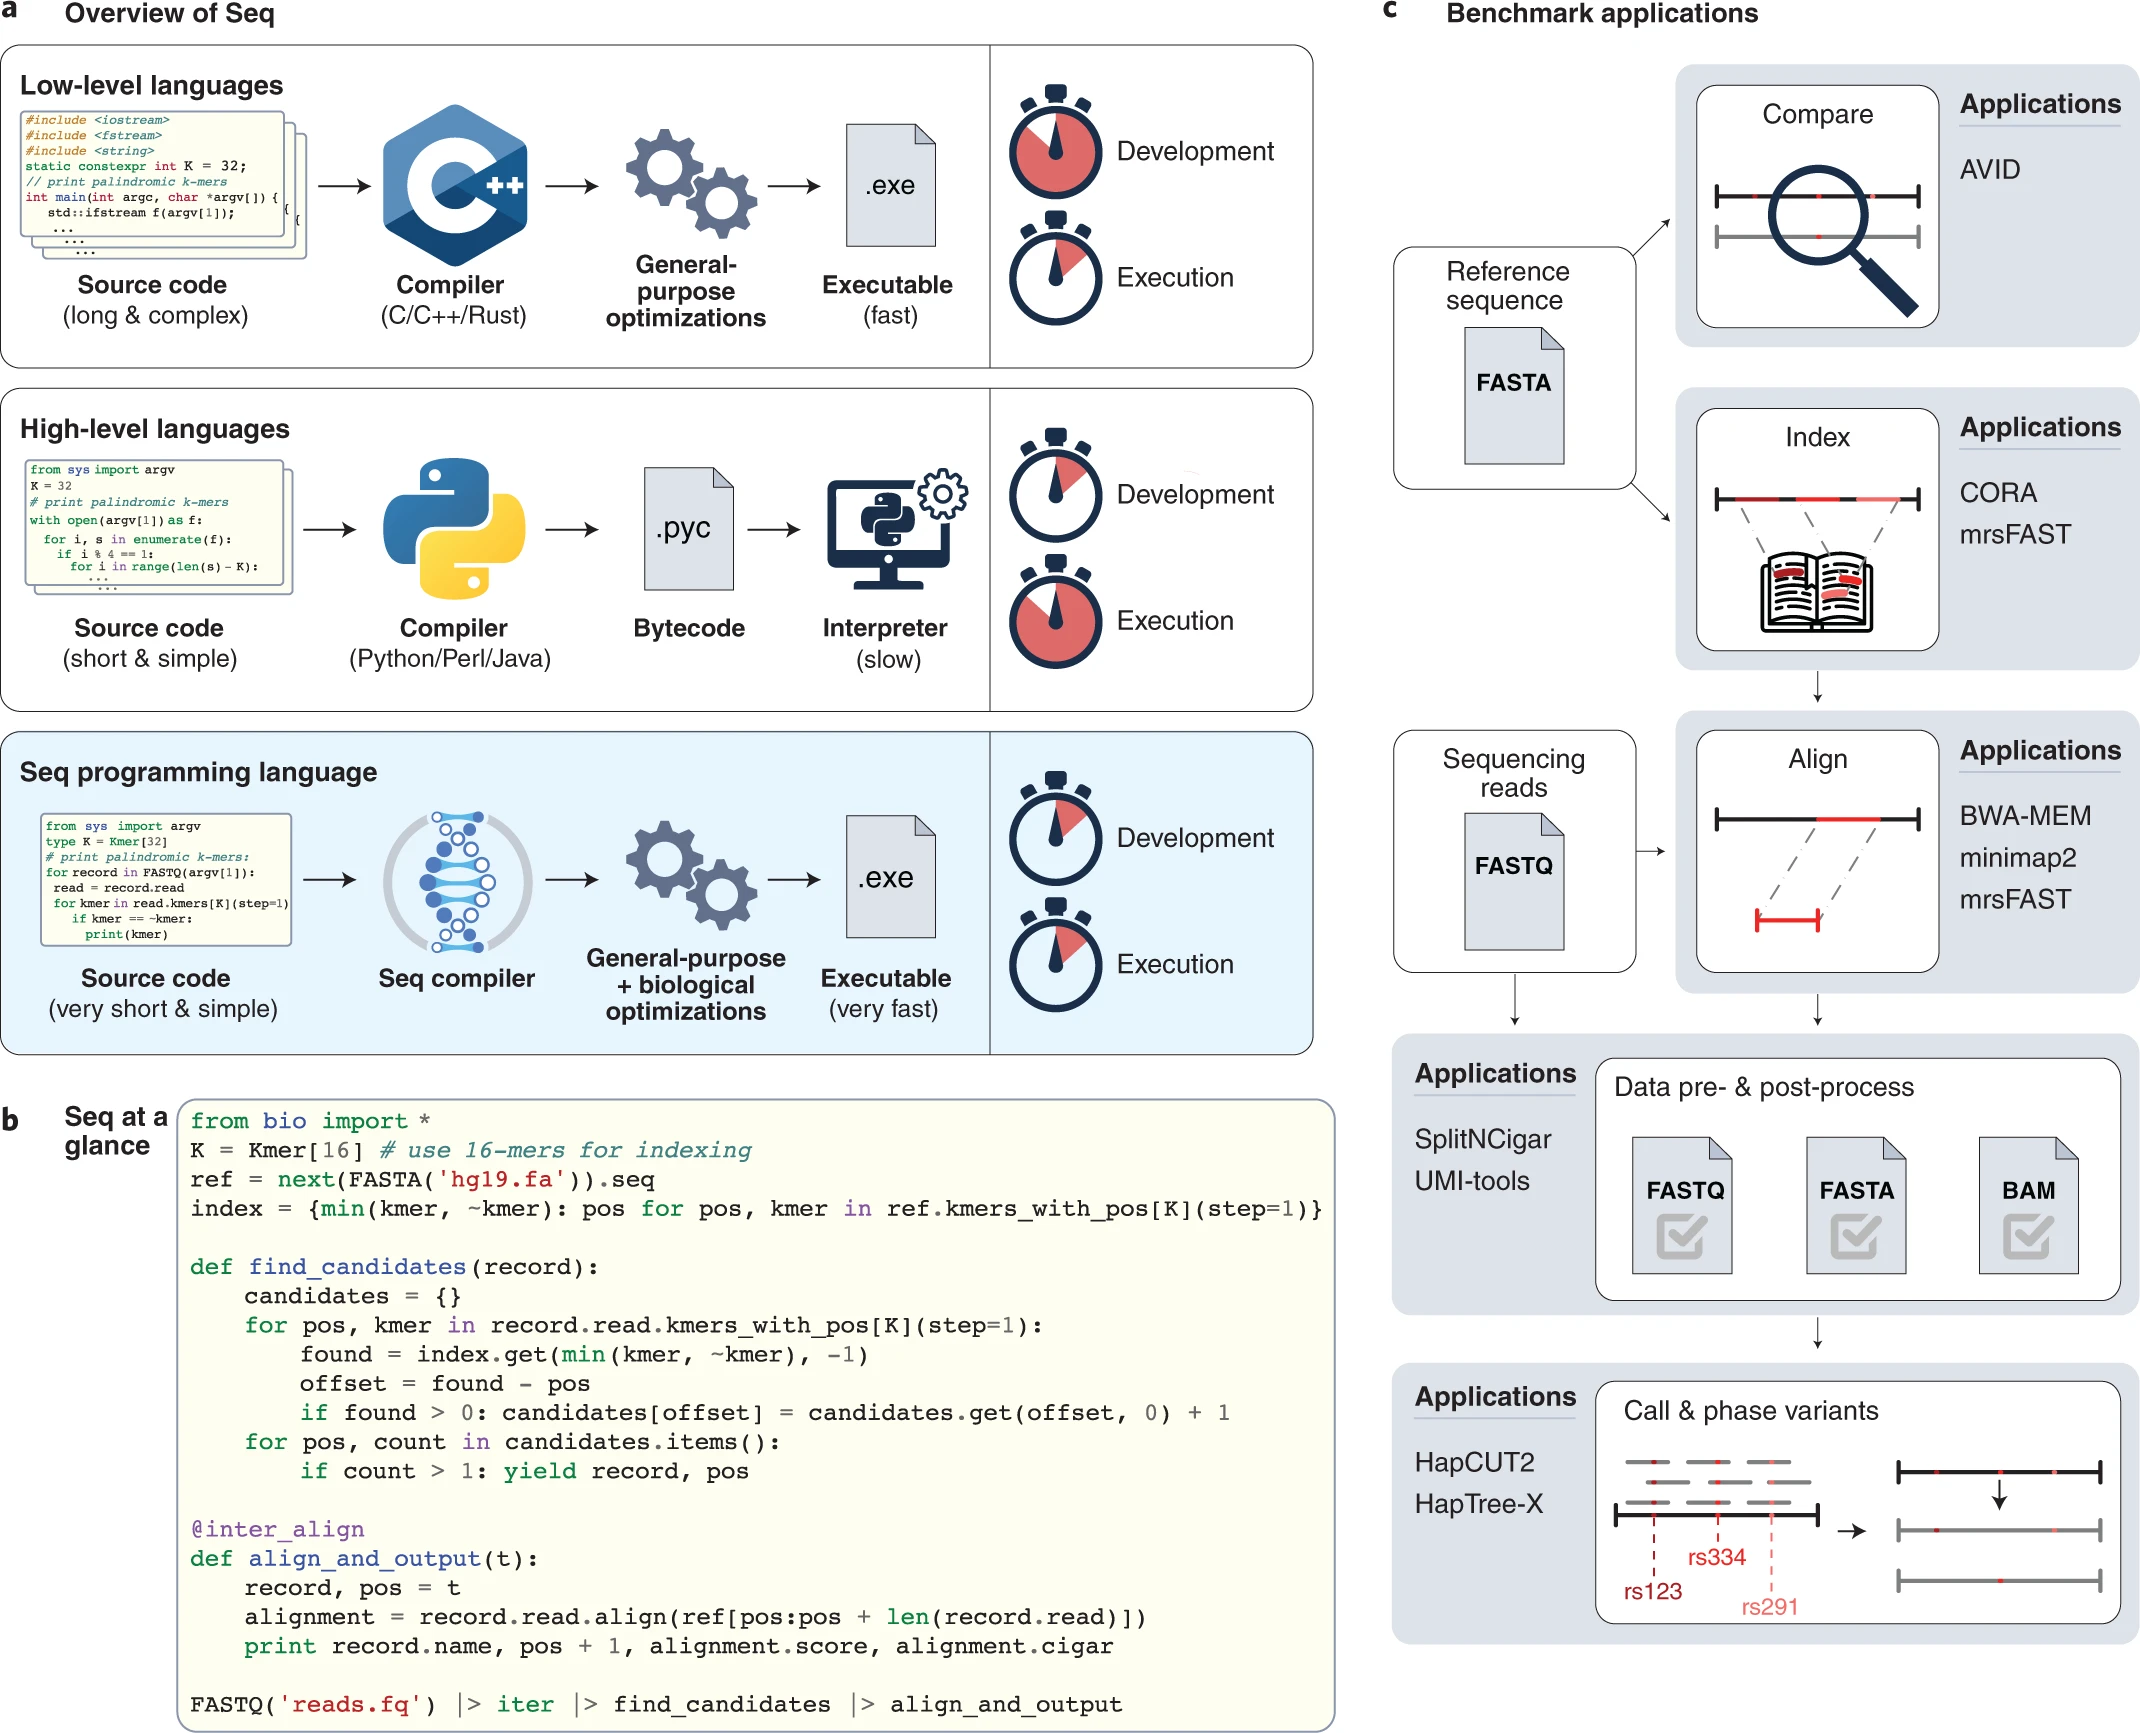
\includegraphics{./figs/computationalBio/The Seq programming language.jpg}
\caption{The Seq programming language.}
\end{figure}

a, Conceptual comparison of Seq, Python and C++. Seq combines the high performance of C++ with the programming ease and clarity of Python, by virtue of domain-specific compiler optimizations that are hidden from the user. b, Example Seq code for a simple k-mer-based read mapper. c, Schematic of standard genomics pipeline and those state-of-the-art tools compared to Seq.

To demonstrate Seq's versatility, we reimplemented eight popular genomics tools in Seq, spanning key tasks in the genomics analysis pipeline (Fig. 1c and Supplementary Note 2), such as the finding of super-maximal exact matches, or SMEMs (BWA-MEM13), genome homology table construction (CORA14), Hamming distance-based all-mapping (mrsFAST15), long-read alignment (minimap216), \textbf{single-cell data preprocessing (UMI-tools17)}, SAM/BAM post-processing (GATK18), global sequence alignment (AVID19) and \textbf{haplotype phasing (Haptree-X20,21)}.

\href{https://github.com/seq-lang/seq-benchmarks/tree/master/seq-nbt\#haptree-x-haplotype-phasing}{Hap Tree-X}

\hypertarget{singlecell-analysis-tools}{%
\section{singlecell analysis tools}\label{singlecell-analysis-tools}}

\begin{itemize}
\item
  scanpy
  \href{https://genomebiology.biomedcentral.com/articles/10.1186/s13059-017-1382-0}{SCANPY: large-scale single-cell gene expression data analysis}
\item
  seurat
\end{itemize}

\hypertarget{singlecell-analysis-sources}{%
\section{singlecell analysis sources}\label{singlecell-analysis-sources}}

\hypertarget{spatial-technology}{%
\chapter{Spatial Technology}\label{spatial-technology}}

\hypertarget{sequencing-based-st}{%
\section{Sequencing based ST}\label{sequencing-based-st}}

\hypertarget{statmethods}{%
\chapter{StatMethods}\label{statmethods}}

\hypertarget{hmm-based-methods}{%
\section{HMM based methods}\label{hmm-based-methods}}

\hypertarget{em-based-methods}{%
\section{EM based methods}\label{em-based-methods}}

\hypertarget{vb-based-methods}{%
\section{VB based methods}\label{vb-based-methods}}

\hypertarget{glm}{%
\section{GLM}\label{glm}}

\href{https://www.statsmodels.org/stable/glm.html\#links}{statsmodel GLM}

\href{https://www.statsmodels.org/stable/generated/statsmodels.discrete.discrete_model.NegativeBinomial.html}{statsmodels.discrete.discrete\_model.NegativeBinomial}

\hypertarget{phd-research-topic-based}{%
\chapter{PhD Research topic based}\label{phd-research-topic-based}}

\hypertarget{cnv-calling}{%
\section{CNV calling}\label{cnv-calling}}

\hypertarget{breaking-point-detection}{%
\subsection{breaking point detection}\label{breaking-point-detection}}

\begin{itemize}
\tightlist
\item
  4 CNV breakpoint detection methods (2021-07-17 Group meeting)
\end{itemize}

\begin{enumerate}
\def\labelenumi{\arabic{enumi}.}
\tightlist
\item
  CHISEL: \url{https://www.nature.com/articles/s41587-020-0661-6\#Sec8} (see global clustering subsection)
\end{enumerate}

\begin{itemize}
\tightlist
\item
  seemingly no breakpoint detection, but rather a global clustering (ie. entry-wise for a bin-by-cell matrix), thus the resolution of CNV is the bin size (5MB)
\end{itemize}

\begin{enumerate}
\def\labelenumi{\arabic{enumi}.}
\setcounter{enumi}{1}
\tightlist
\item
  Alleloscope: \url{https://www.nature.com/articles/s41587-021-00911-w\#Sec10} (see segmentation subsection)
\end{enumerate}

\begin{itemize}
\tightlist
\item
  HMM on a pooled cells (pseudo-bulk?) with pre-defined Gaussian means and variance for each state
\end{itemize}

\begin{enumerate}
\def\labelenumi{\arabic{enumi}.}
\setcounter{enumi}{2}
\tightlist
\item
  InferCNV: \url{https://github.com/broadinstitute/inferCNV/wiki/inferCNV-HMM-based-CNV-Prediction-Methods}
\end{enumerate}

\begin{itemize}
\tightlist
\item
  i6-HMM generates in silico spike-in; seemingly define CNV region (segment) on cluster instead of cell, but using noise model on each cell (not quite sure from the doc).
\end{itemize}

\begin{enumerate}
\def\labelenumi{\arabic{enumi}.}
\setcounter{enumi}{3}
\tightlist
\item
  CopyKat: \url{https://www.nature.com/articles/s41587-020-00795-2\#Sec9}
\end{enumerate}

\begin{itemize}
\tightlist
\item
  KS test for whether to two neighbour bins should be joined, by using the posterior samples of Gamma-Poisson posterior. Seemingly using noise model on each cell within a cluster
\end{itemize}

FACLON
\url{https://academic.oup.com/nar/article/43/4/e23/2410993}

\begin{figure}
\centering
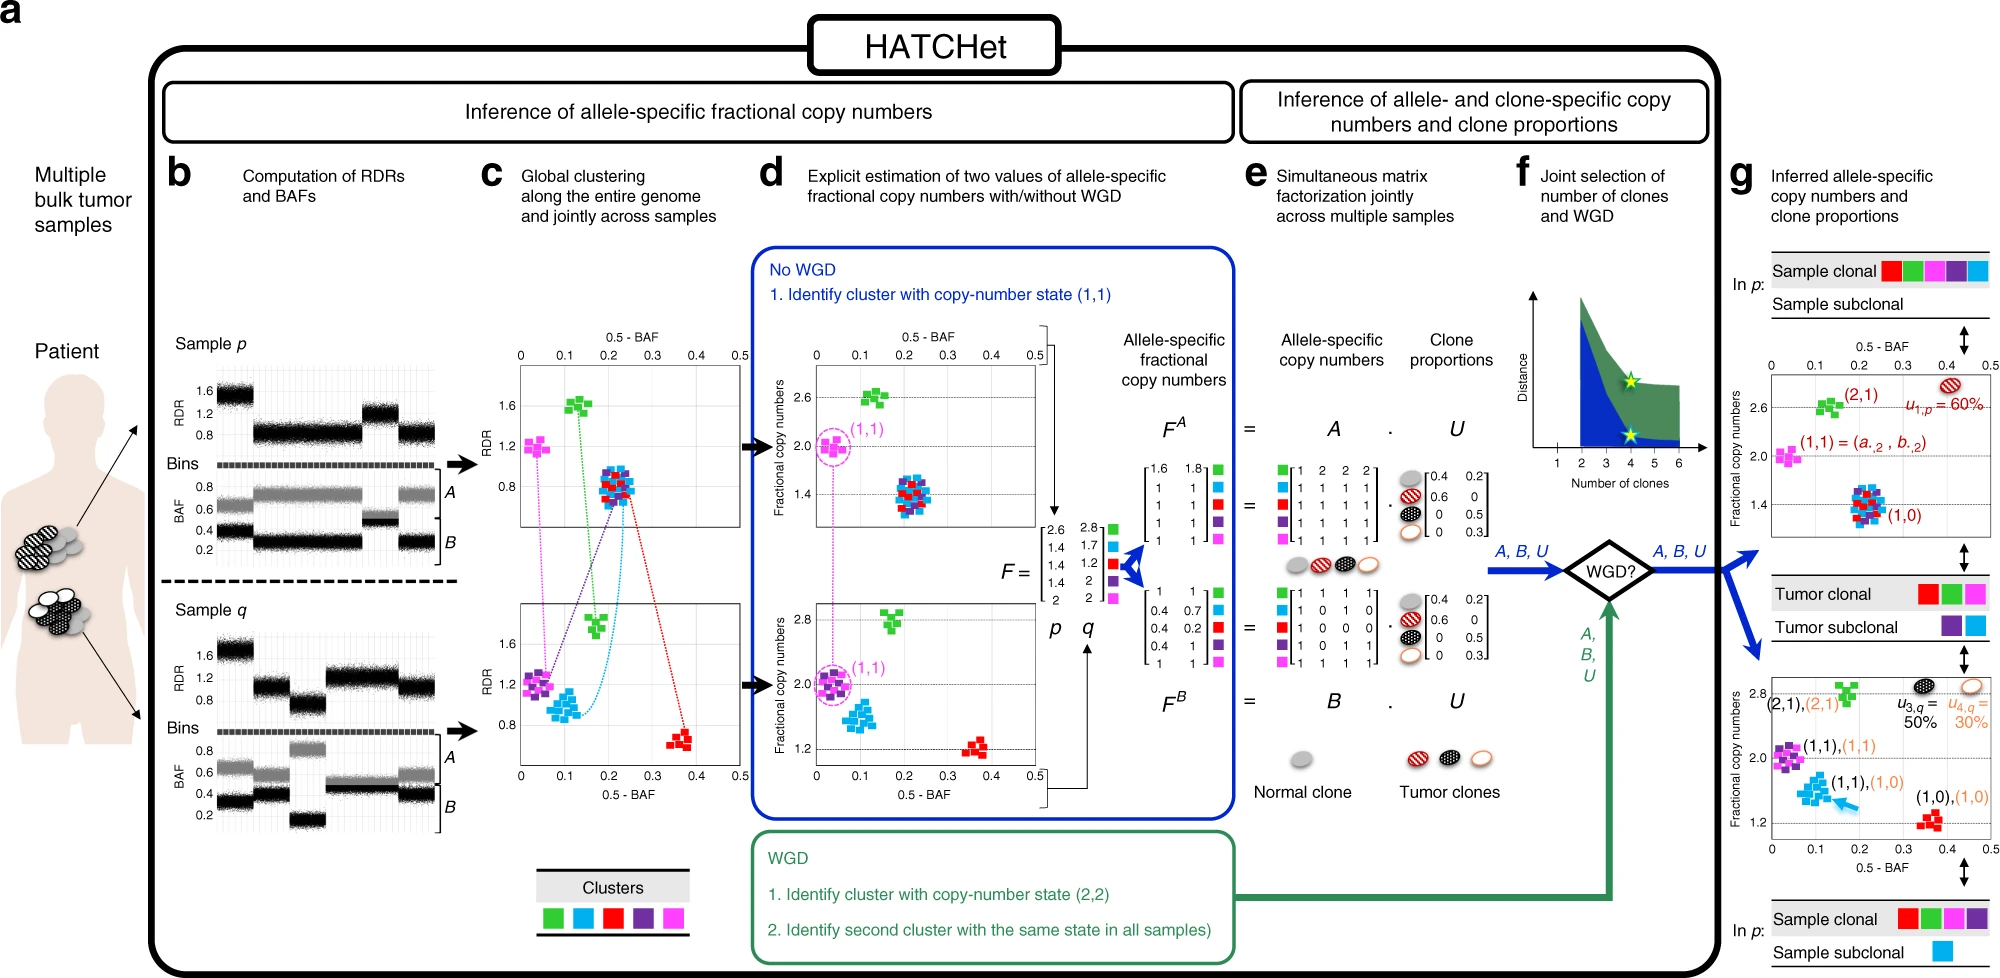
\includegraphics{./figs/CNV/HATCHet.jpg}
\caption{Overview of HATCHet algorithm}
\end{figure}

\url{https://www.nature.com/articles/s41467-020-17967-y/figures/1}

\textbf{a} HATCHet takes in input DNA sequencing data from multiple bulk tumor samples of the same patient and has five steps.
\textbf{b} First, HATCHet calculates the RDRs and BAFs in bins of the reference genome (black squares). Here, we show two tumor samples p and q.
\textbf{c} Second, HATCHet clusters the bins based on RDRs and BAFs globally along the entire genome and jointly across samples p and q. Each cluster (color) includes bins with the same copy-number state within each clone present in p or q.
\textbf{d} Third, HATCHet estimates two values for the fractional copy number of each cluster by scaling RDRs. If there is no WGD, the identification of the cluster (magenta) with copy-number state (1, 1) is sufficient and RDRs are scaled correspondingly.
If a WGD occurs, HATCHet identifies an additional cluster with identical copy-number state in all tumor clones. Dashed black horizontal lines in the scaled BAF-RDR plot represent values of fractional copy numbers that correspond to clonal CNAs.
\textbf{e} Fourth, HATCHet factors the allele-specific fractional copy numbers FA, FB into the allele-specific copy numbers A, B, respectively, and the clone proportions U. Here, there is a normal clone and 3 tumor clones.
\textbf{f} Last, HATCHet's model-selection criterion identifies the matrices A, B, and U in the factorization while evaluating the fit according to both the inferred number of clones and presence/absence of a WGD.
\textbf{g} HATCHet outputs allele- and clone-specific copy numbers (with the color of the corresponding clone) and clone proportions (in the top right part of each plot) for each sample.
Clusters are classified according to the inference of unique/different copy-number states in each sample (sample-clonal/subclonal) and across all tumor clones (tumor-clonal/subclonal).

\begin{figure}
\centering
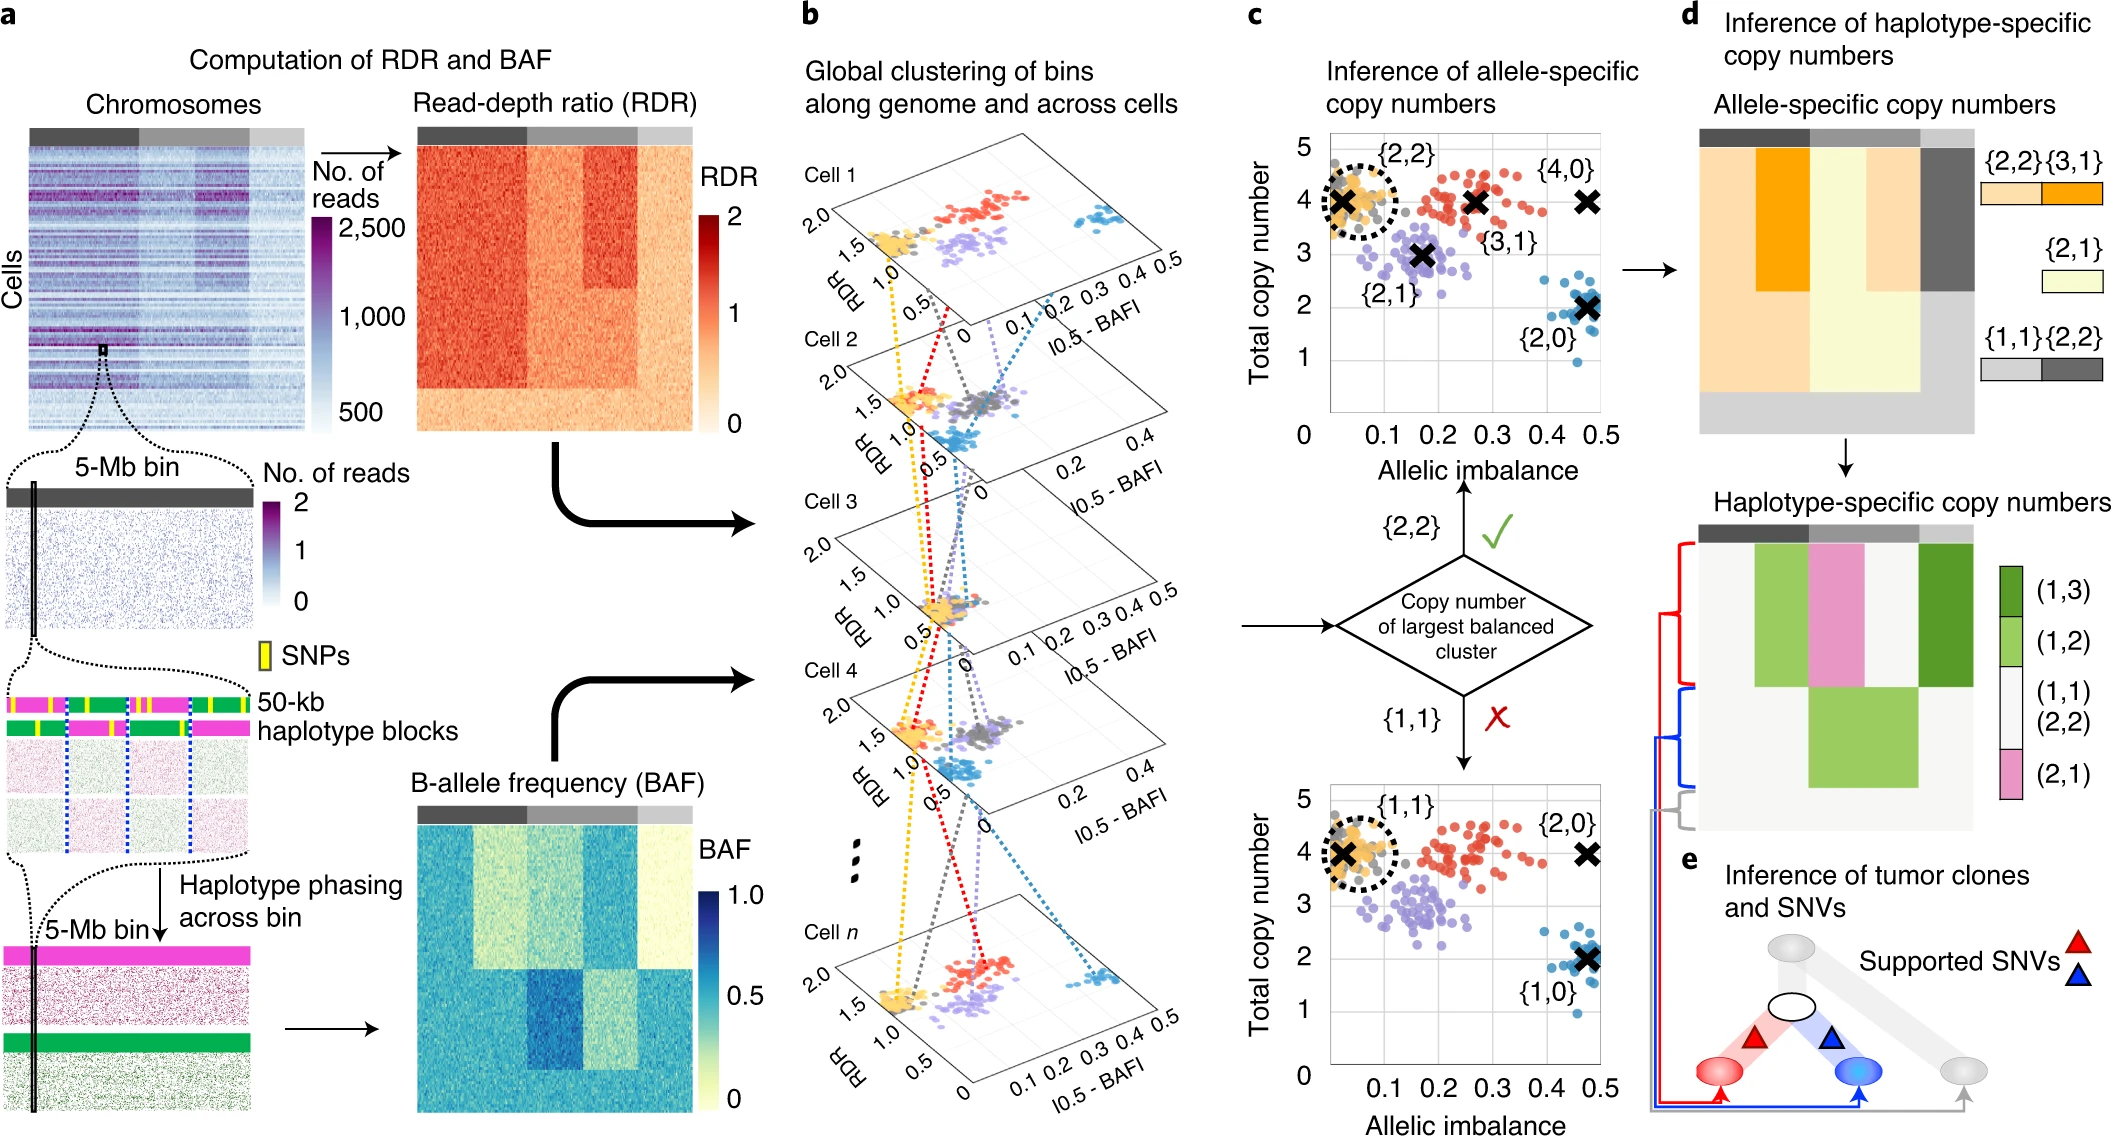
\includegraphics{./figs/CNV/chisel.jpg}
\caption{Overview of chisel algorithm}
\end{figure}

\url{https://www.nature.com/articles/s41587-020-0661-6/figures/1}

\textbf{a}, CHISEL computes RDRs and BAFs in low-coverage (\textless0.05× per cell) single-cell DNA sequencing data (top left). Read counts from 2,000 individual cells (rows) in 5-Mb genomic bins (columns) across three chromosomes (gray rectangles in first row) are shown.
For each bin in each cell, CHISEL computes the RDR (top) by normalizing the observed read counts. CHISEL computes the BAF in each bin and cell (bottom) by first performing referenced-based phasing of germline SNPs in 50-kb haplotype blocks (magenta and green) and then phasing all these blocks jointly across all cells.
\textbf{b}, CHISEL clusters RDRs and BAFs globally along the genome and jointly across all cells resulting here in five clusters of genomic bins (red, blue, purple, yellow and gray) with distinct copy-number states.
\textbf{c}, CHISEL infers a pair \{c\^{}t,cˇt\} of allele-specific copy numbers for each cluster by determining whether the allele-specific copy numbers of the largest balanced (BAF of \textasciitilde0.5) cluster are equal to \{1, 1\} (diploid), \{2, 2\} (tetraploid) or are higher ploidy.
\textbf{d}, CHISEL infers haplotype-specific copy numbers (at, bt) by phasing the allele-specific copy numbers \{c\^{}t,cˇt\} consistently across all cells.
\textbf{e}, CHISEL clusters tumor cells into clones according to their haplotype-specific copy numbers. Here, a diploid clone (light gray) and two tumor clones (red and blue) are obtained.
A phylogenetic tree describes the evolution of these clones. Somatic SNVs are derived from pseudo-bulk samples and placed on the branches of the tree.

\begin{figure}
\centering
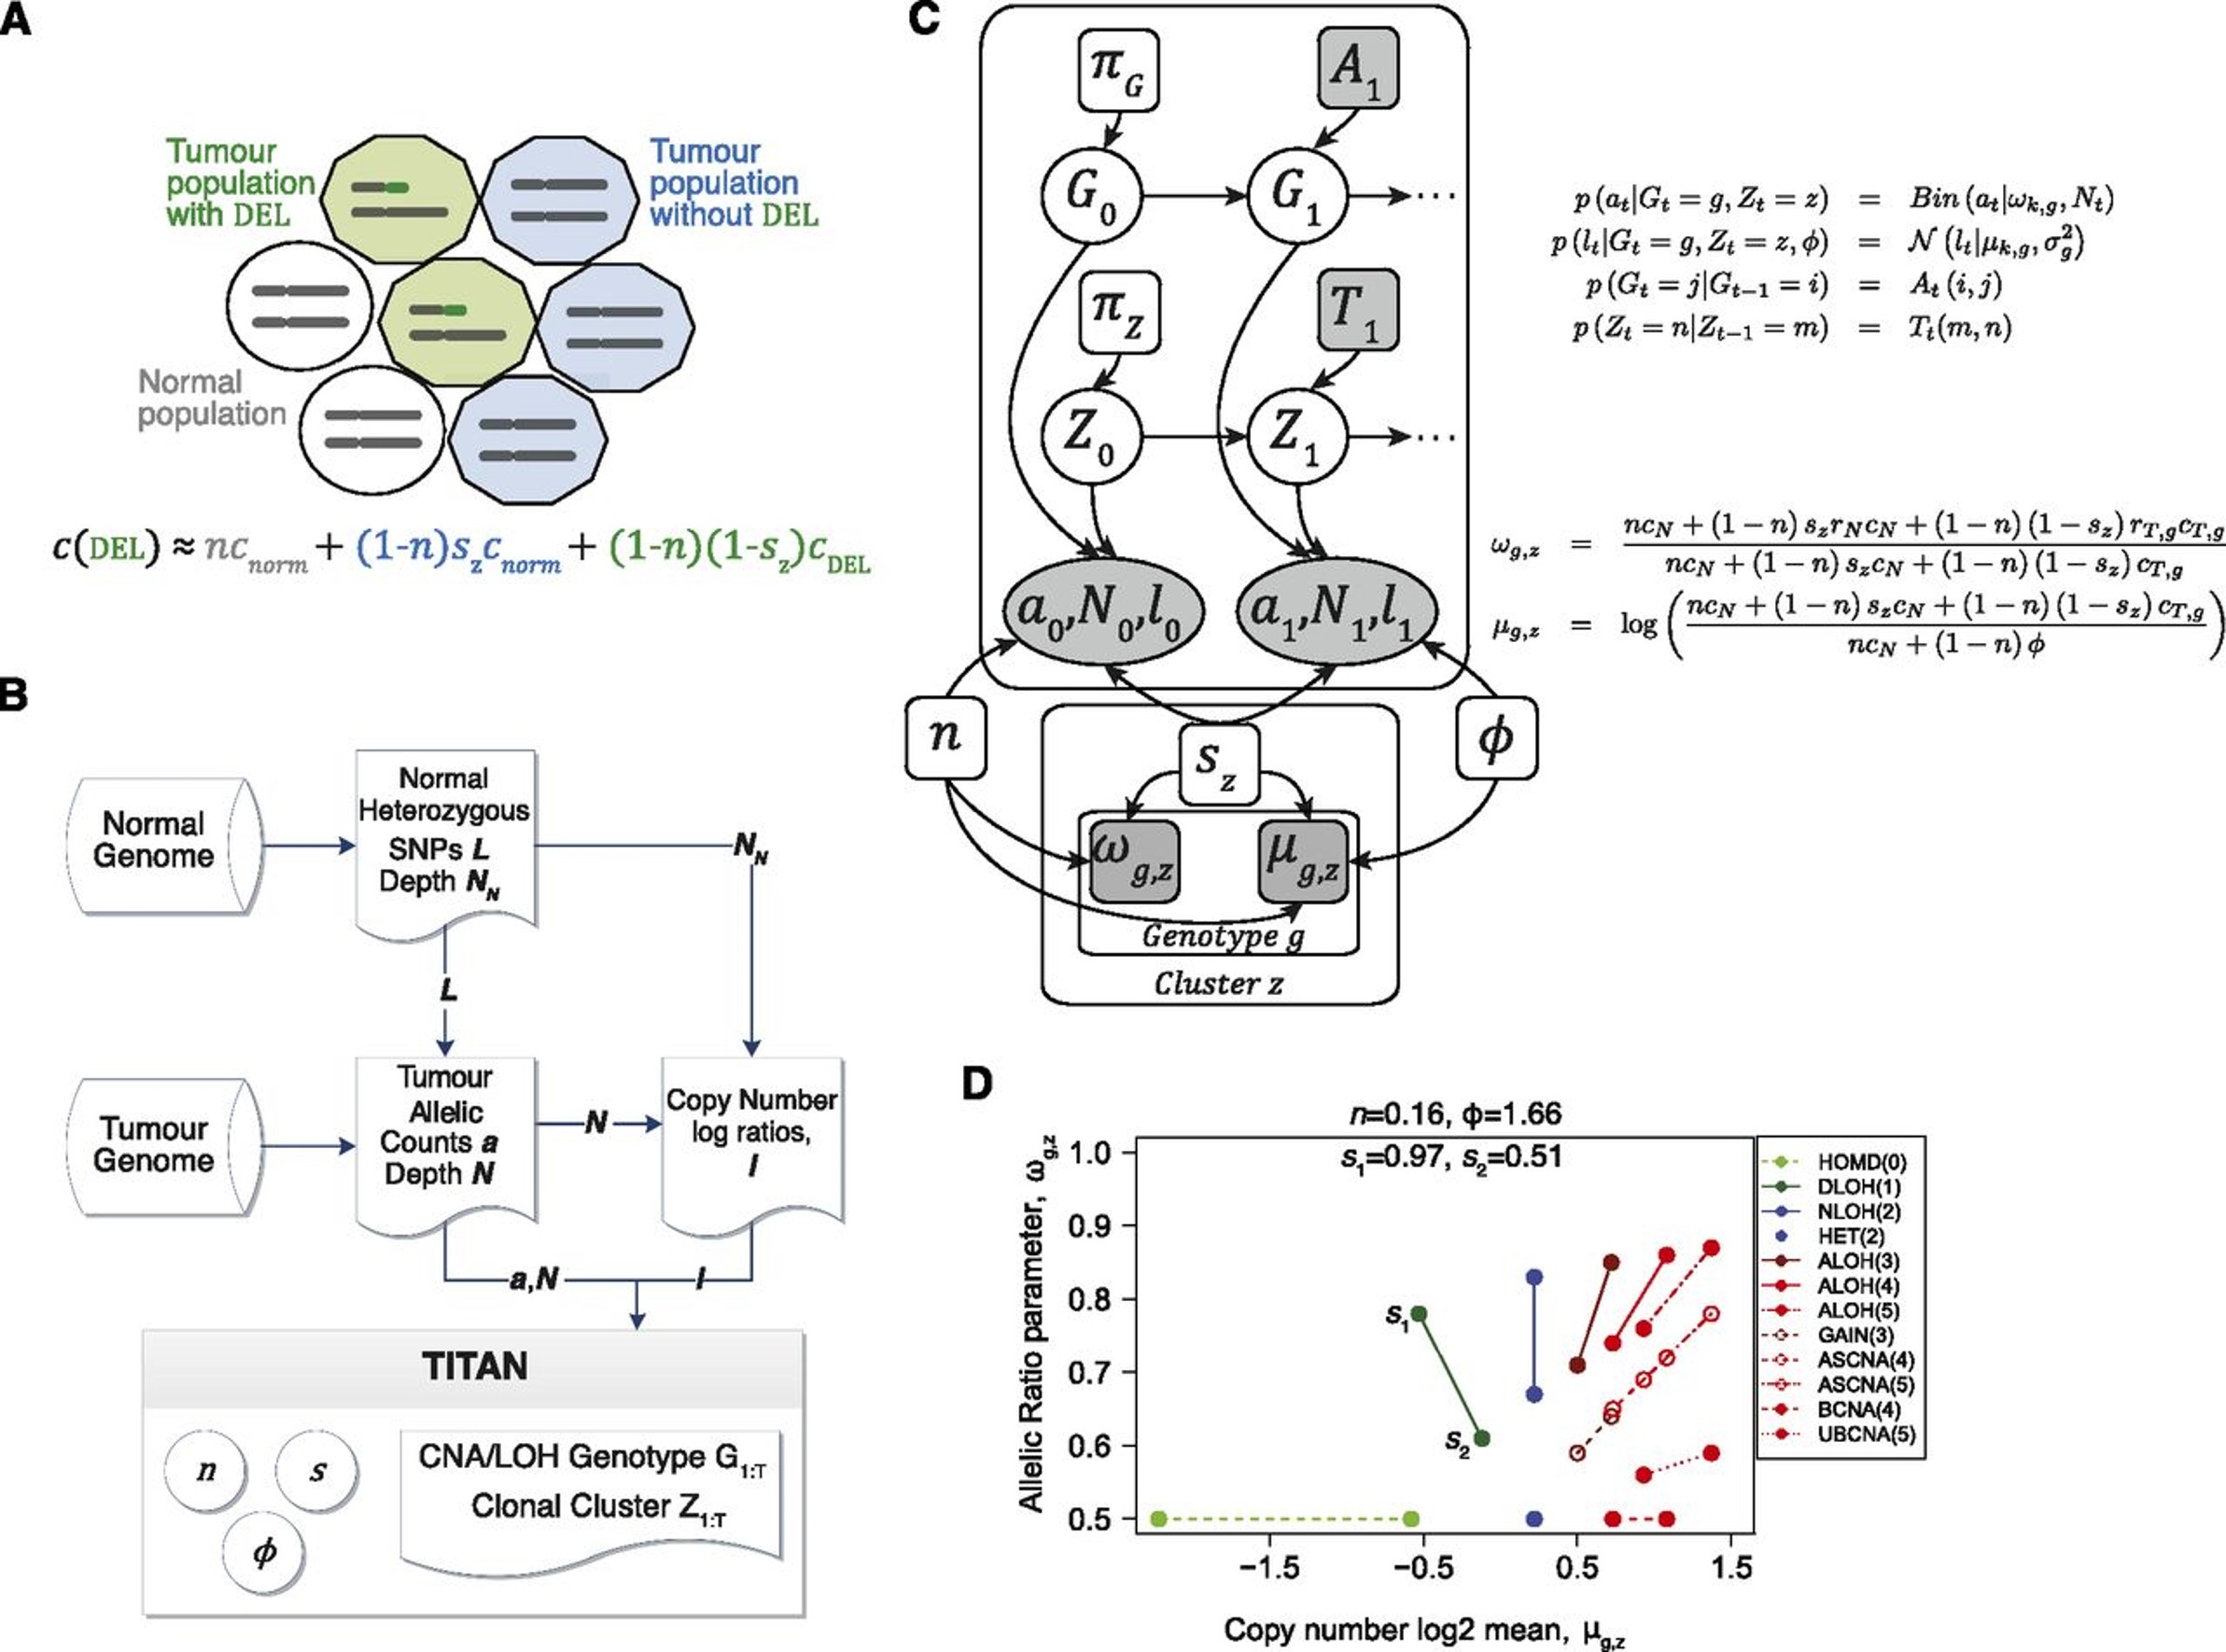
\includegraphics{./figs/CNV/TITAN.jpg}
\caption{Overview of TITAN local clustering for segemetation}
\end{figure}

\begin{figure}
\centering
\includegraphics{./figs/CNV/infercnv_i3HMM_model.png}
\caption{Overview of inferCNV i3HMM}
\end{figure}

\begin{figure}
\centering
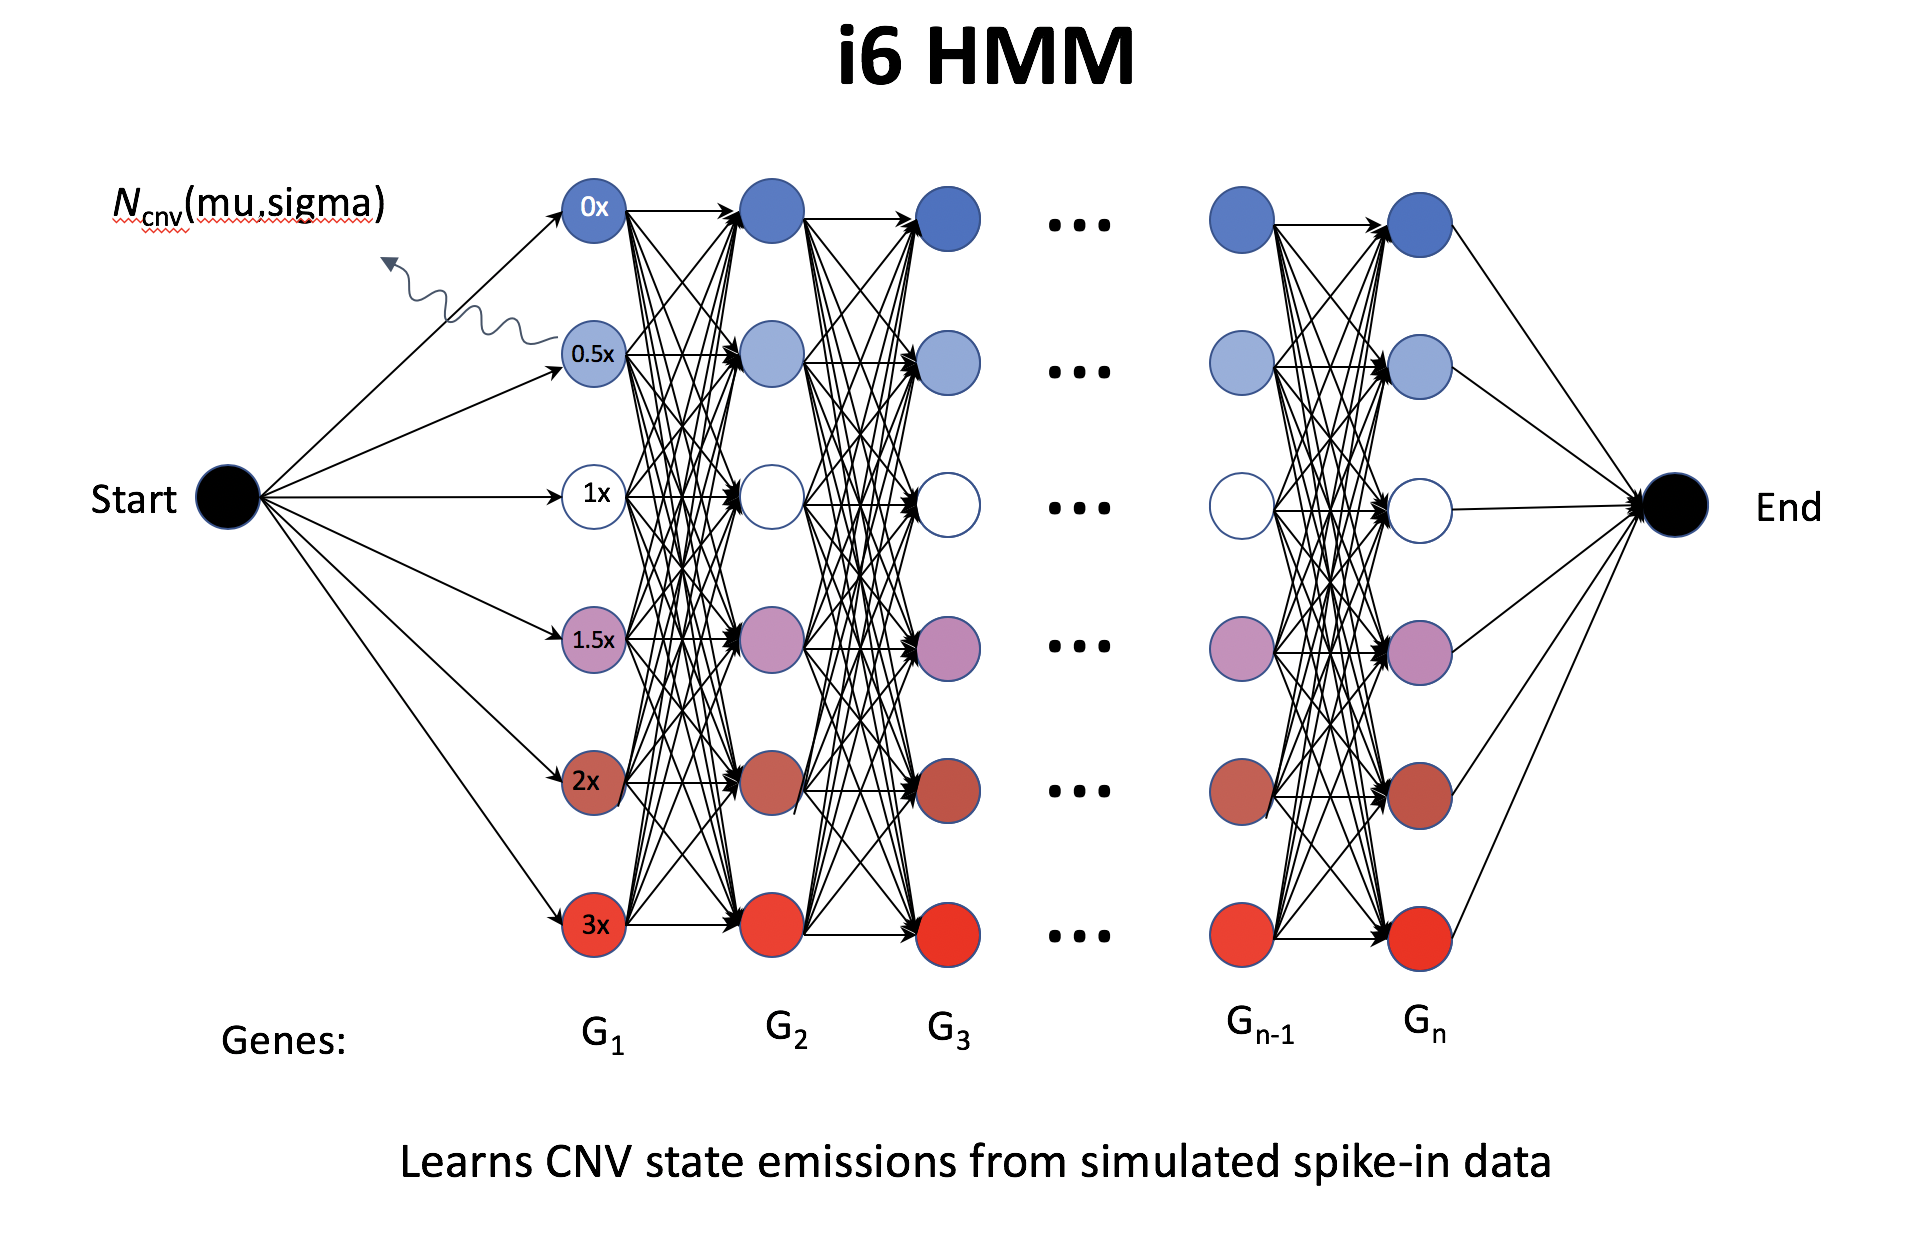
\includegraphics{./figs/CNV/infercnv_i6HMM_model.png}
\caption{Overview of inferCNV i6HMM}
\end{figure}

\begin{figure}
\centering
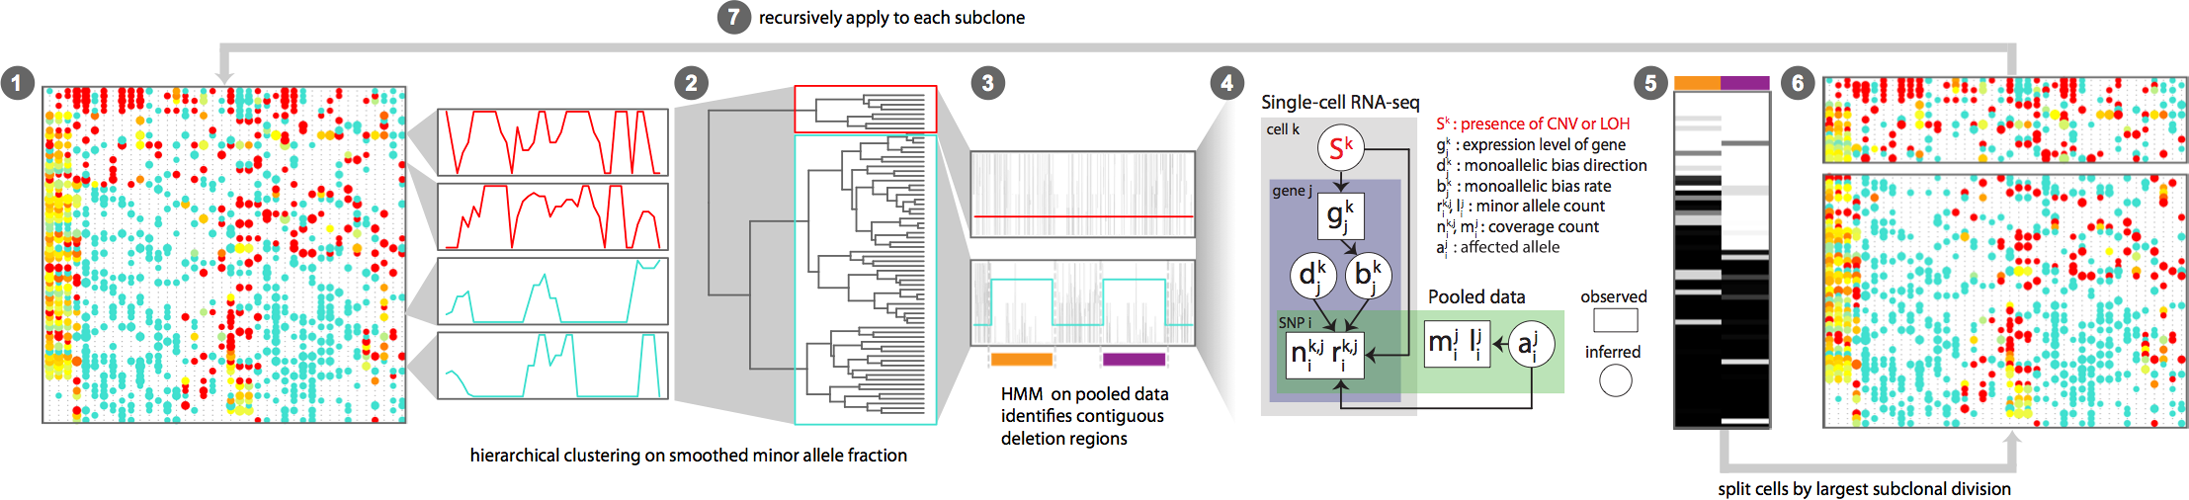
\includegraphics{./figs/CNV/HoneyBADGER.png}
\caption{Overview of HoneyBADGER method}
\end{figure}

\begin{figure}
\centering
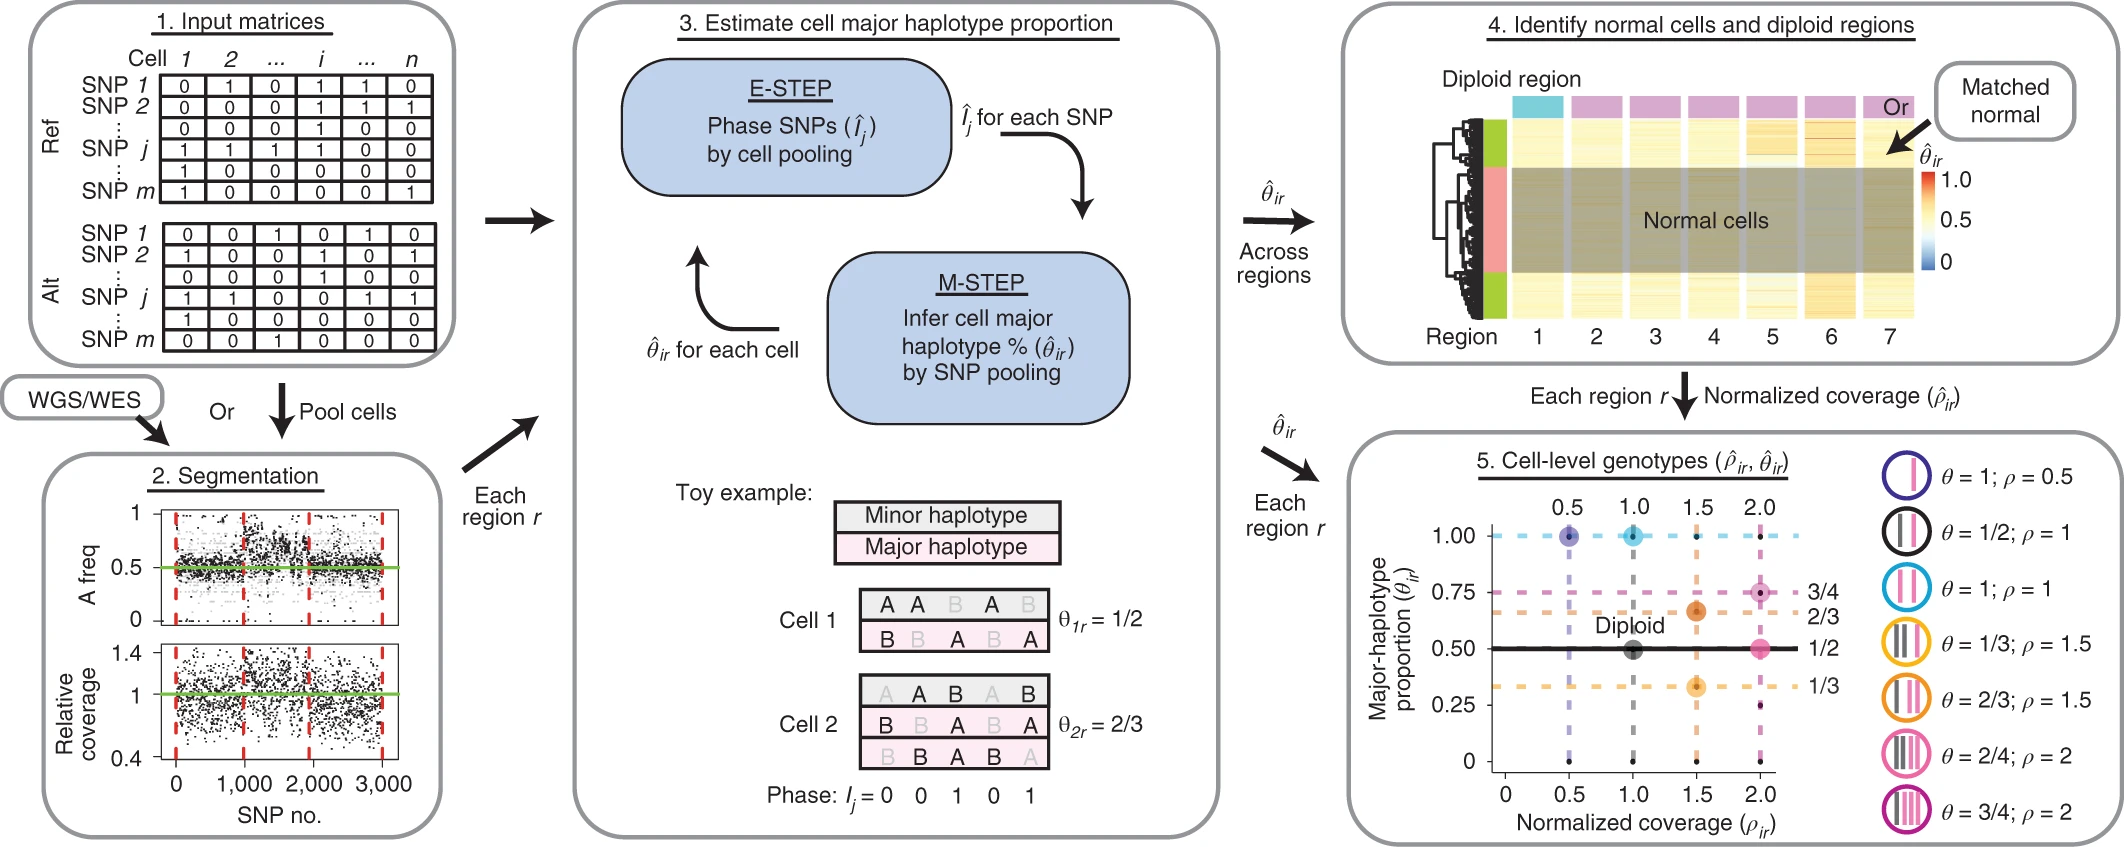
\includegraphics{./figs/CNV/Alleloscope.jpg}
\caption{Overview of Alleloscope algorithm}
\end{figure}

\begin{figure}
\centering
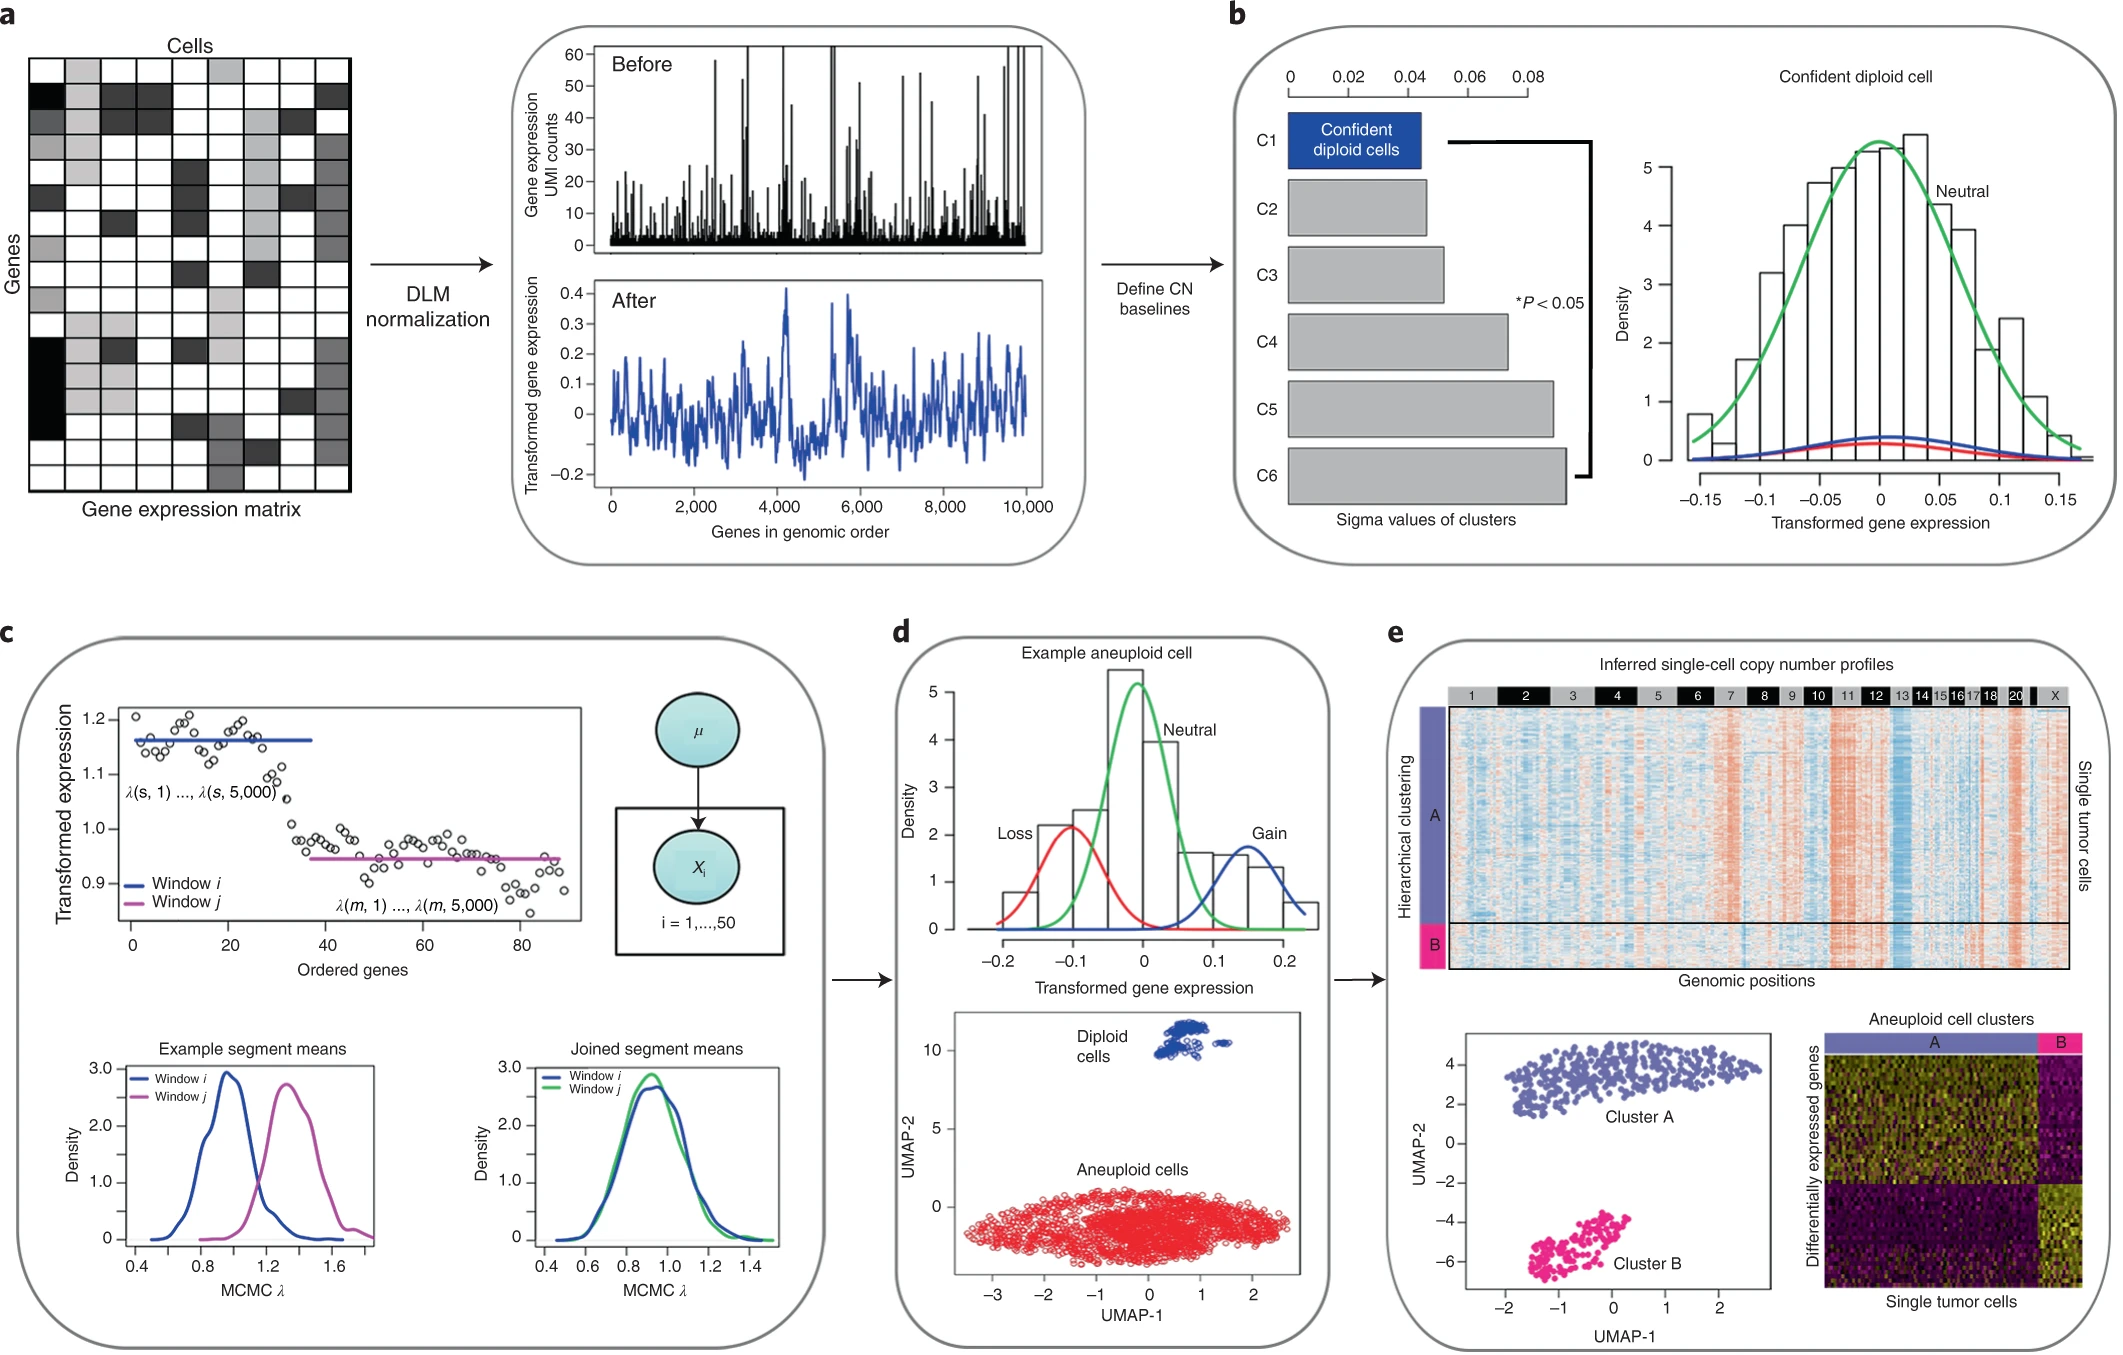
\includegraphics{./figs/CNV/copykat.jpg}
\caption{Overview of copykat algorithm}
\end{figure}

\hypertarget{related-research}{%
\subsection{Related research}\label{related-research}}

\textbf{clonealign}: statistical integration of independent single-cell RNA and DNA sequencing data from human cancers

However, independently sampled single-cell measurements introduce a new analytical challenge of how to associate cells across each modality. Assuming a population structure with a fixed number of clones, this can be expressed as a mapping problem, whereby cells measured with transcriptome assays must be aligned to those measured with a genome assay.

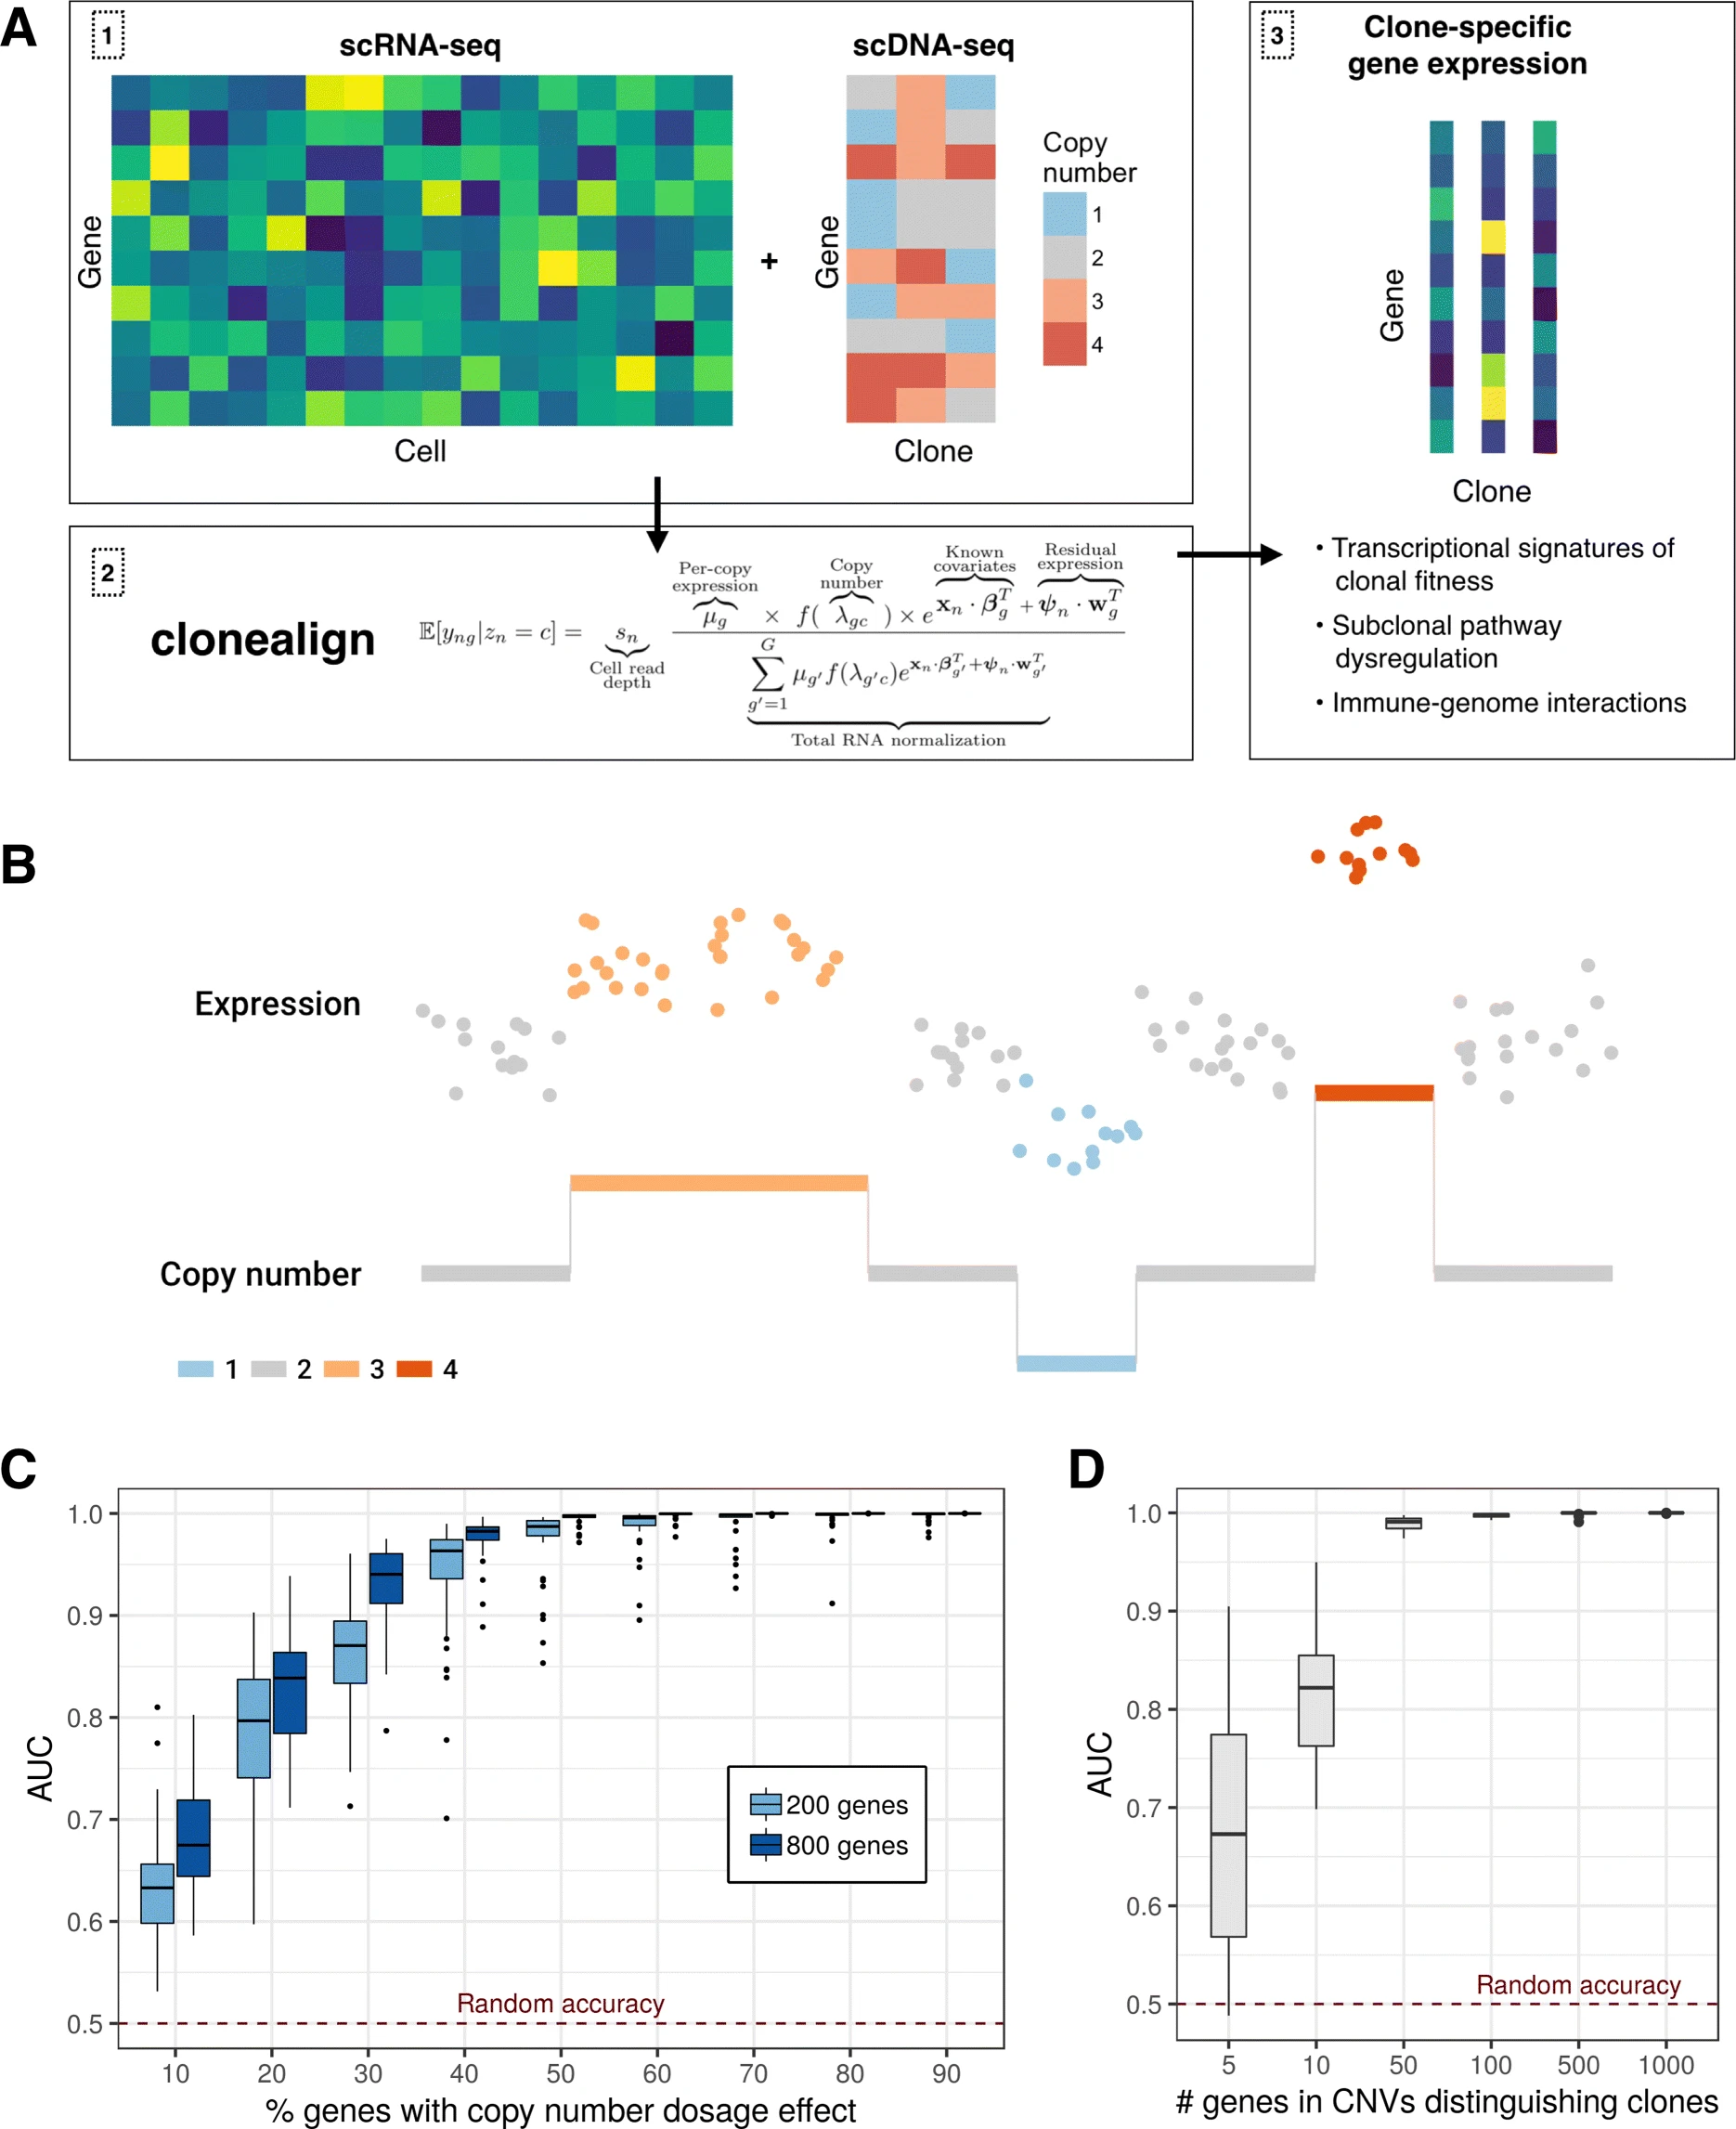
\includegraphics{./figs/CNV/clonealign.jpg}
In order to relate the independent measurements, we assume that an increase in the copy number of a gene will result in a corresponding increase in that gene's expression and vice versa (Fig. 1b)
a relationship previously observed in joint RNA-DNA assays in bulk tissues {[}12{]} and at the single-cell level {[}9, 10, 13{]}.

\textbf{CHISEL}

\textbf{inferCNV}

\textbf{copyKAT}

\textbf{CaSpER}

\textbf{HoneyBADGER}

\hypertarget{smoothing-strategies-in-rdr}{%
\subsection{Smoothing strategies in RDR}\label{smoothing-strategies-in-rdr}}

-TODO

\hypertarget{pubmon}{%
\subsection{PUBMON}\label{pubmon}}

\href{https://www.biorxiv.org/content/10.1101/2021.11.25.469995v1}{Precise identification of cancer cells from allelic imbalances in single cell transcriptomes}

this paper used BAF information to identify cancer cells, seems quite relevant.

\textbf{2022-03-09}

\href{https://www.biorxiv.org/content/10.1101/2021.06.04.447031v1.full}{Evolutionary tracking of cancer haplotypes at single-cell resolution}

\href{https://www.biorxiv.org/content/10.1101/2022.02.07.479314v1.full}{Haplotype-enhanced inference of somatic copy number profiles from single-cell transcriptomes}

\begin{itemize}
\item
  \textbf{Numbat}
\item
  introduction
\end{itemize}

Existing approaches for CNV detection from scRNA-seq do not utilize the prior knowledge of haplotypes, or the individual-specific configuration of variant alleles on the two homologous chromosomes, which can enable more sensitive detection of allelic imbalance.

The utility of phasing in detecting CNV signals from scRNA-based assays, however, has not been explored.

We therefore developed a computational method, Numbat, which integrates expression, allele, and haplotype information derived from population-based phasing to comprehensively characterize the CNV landscape in single-cell transcriptomes.

Numbat does not require sample-matched DNA data or a priori genotyping, and is widely applicable to a wide range of experimental settings and cancer types.

\begin{itemize}
\tightlist
\item
  Results
\end{itemize}

\textbf{Enhanced detection of subclonal allelic imbalances using population-based haplotype phasing}

Prior phasing information can effectively amplify weak allelic imbalance signals of individual SNPs induced by the CNV, by exposing joint behavior of entire haplotype sequences and thereby increasing the statistical power.

The ability to infer phasing between genes is particularly useful for CNV inference, as it provides means to overcome stochastic allele-specific expression effects which give rise to bursts of gene-specific allelic imbalances in individual cells.

The differential phasing accuracy from within and between genes reflects the fact that the strength of genetic linkage decays with increasing distance (Supplementary Figure 1a).

To reflect the decay in phasing strength over longer genetic distances, we introduced site-specific transition probabilities between haplotype states in the Numbat allele HMM (see Methods).

\textbf{Accurate copy number inference from single-cell transcriptomes}

To increase robustness, Numbat models gene expression as integer read counts using a discrete Poisson Lognormal mixture distribution, and accounts for excess variance in the allele frequency (e.g.~due to allele-specific detection or transcriptional bursts) using a Beta-Binomial distribution.

\textbf{Iterative strategy to decompose tumor clonal architecture}

\textbf{Reliable identification of cancer cells in the tumor microenvironment}

\textbf{Allele-specific CNV analysis reveals additional subclonal complexity}

\textbf{Unraveling the interplay between genetic and transcriptional heterogeneity in tumor evolution}

\begin{itemize}
\item
  Discussion
\item
  Methods
\end{itemize}

\hypertarget{clonal-tree}{%
\section{Clonal Tree}\label{clonal-tree}}

\hypertarget{deconvolution}{%
\section{Deconvolution}\label{deconvolution}}

\hypertarget{deconvolution-of-bulk-tissue-and-spatial-transcriptomic-data}{%
\subsection{Deconvolution of bulk tissue and spatial transcriptomic data}\label{deconvolution-of-bulk-tissue-and-spatial-transcriptomic-data}}

Related papers are as follows:

\begin{itemize}
\tightlist
\item
  \href{https://www.nature.com/articles/s41587-019-0114-2}{CIBERSORTx}
\item
  \href{https://www.nature.com/articles/s41587-021-00830-w}{RCTD}
\item
  \href{https://academic.oup.com/nar/article/49/9/e50/6129341}{SPOTlight}
\item
  \href{https://genomebiology.biomedcentral.com/articles/10.1186/s13059-021-02362-7}{SpatialDWLS}
\end{itemize}

From xiunan's pre

\href{https://www.biorxiv.org/content/10.1101/2021.06.15.448381v1}{Reference-free cell-type deconvolution of pixel-resolution spatially resolved transcriptomics data}

Yuanhua add

\hypertarget{omics-integration}{%
\section{Omics integration}\label{omics-integration}}

\hypertarget{spatial-transcriptomics}{%
\section{Spatial transcriptomics}\label{spatial-transcriptomics}}

\begin{itemize}
\tightlist
\item
  202109 Read in depth (lead by xianjie)
\end{itemize}

\textbf{\href{https://www.biorxiv.org/content/10.1101/2021.07.12.452018v1.full}{The spatial landscape of clonal somatic mutations in benign and malignant tissue}\citep{erickson2021spatial}}

Keywords: CNV

\textbf{\href{https://www.sciencedirect.com/science/article/pii/S0092867420306723}{Multimodal analysis of composition and spatial architecture in human squamous cell carcinoma}\citep{zhang2021supergnova}}

Keywords: alignment of scRNA AND ST

\begin{itemize}
\tightlist
\item
  2022 spatial and CNV
\end{itemize}

\textbf{\href{https://genomebiology.biomedcentral.com/articles/10.1186/s13059-022-02653-7}{Statistical and machine learning methods for spatially resolved transcriptomics data analysis}\citep{zeng2022statistical}}

\textbf{\href{https://pubmed.ncbi.nlm.nih.gov/33022659/}{STARCH: copy number and clone inference from spatial transcriptomics data}\citep{elyanow2021starch}}

\textbf{\href{https://www.biorxiv.org/content/10.1101/2021.07.12.452018v1.abstract}{The spatial landscape of clonal somatic mutations in benign and malignant tissue}\citep{erickson2021spatial}}

Keywords: spatial; CNV

\begin{itemize}
\tightlist
\item
  202409 Review
\end{itemize}

\textbf{\href{https://www.cell.com/cell/fulltext/S0092-8674(24)00834-1}{Spatiotemporal omics for biology and medicine}\citep{liu2024spatiotemporal}}

Keywords: spatial tech

This review offers an updated overview of how spatial omics has advanced our understanding of \textbf{the translation of genetic information into cellular heterogeneity and tissue structural organization and their dynamic changes over time}. It emphasizes the discovery of various biological phenomena, related to organ functionality, embryogenesis, species evolution, and the pathogenesis of diseases.

\begin{figure}
\centering
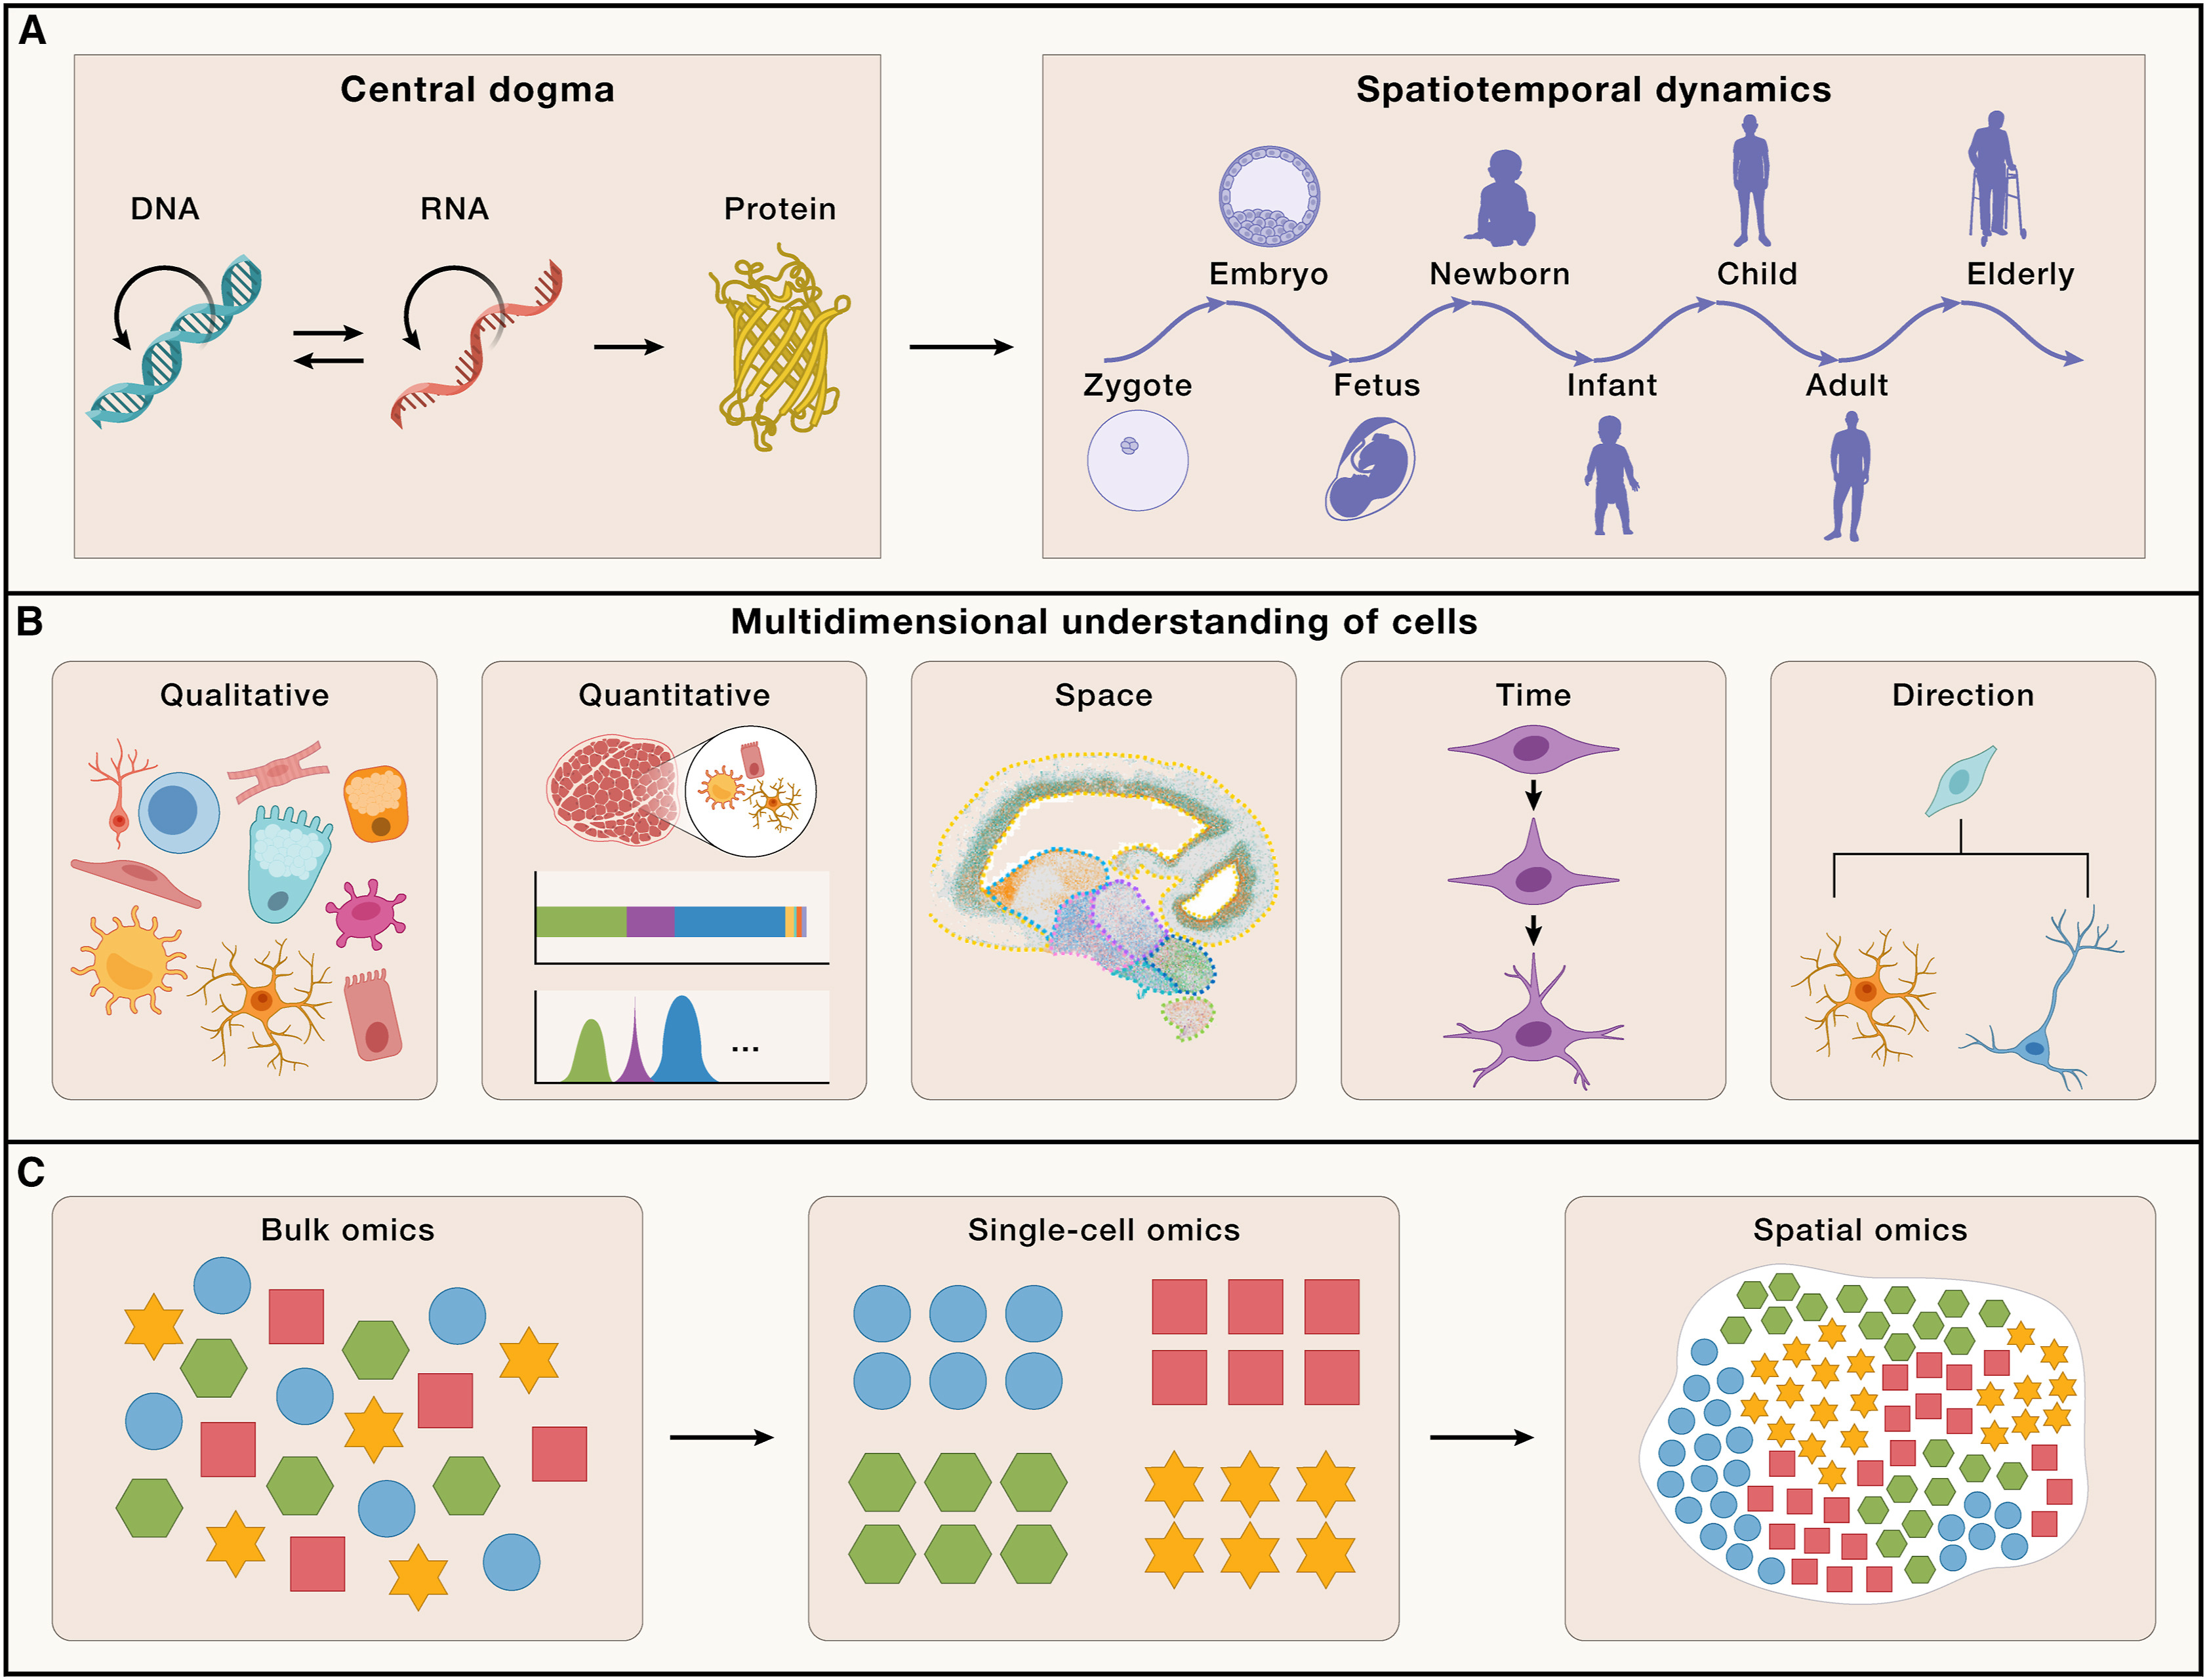
\includegraphics{./figs/spatialtech/Multi-dimensional measurements of cells.jpg}
\caption{Multi-dimensional measurements of cells}
\end{figure}

\textbf{However, a critical question remains about how these variants influence the functions of specific organs or cells.}
Addressing these challenges necessitates a comprehensive understanding of how molecular-level sequence information translates to a single cell within a network of communicating and interacting cells that form functional biological systems. \textbf{This encompasses (1) qualitative-the diversity of cell types generated through the regulation of gene expression; (2) quantitative-the count, proportion, and density of each cell type; (3) space-the spatial arrangement of each cell type and their interactions and cellular ecosystem; (4) time-the specific timing of changes in cell types and states; and (5) direction-the potential transformational paths each cell type may undergo (Figure 1B).}

Understanding these \textbf{multifaceted dimensions of cellular diversity and organization} is crucial for comprehending the connections between the genome and specific biological processes, as well as the regulatory mechanisms involved.

The advances of sequencing technologies, particularly the massively parallel sequencing technology, has enabled large-scale, genome-wide multi-omics analyses of tissues. These methods have revealed pronounced tissue and cell specificity in genetic transcription. However, multi-omics analyses based on bulk tissue primarily capture average-level signals, failing to fully comprehend the heterogeneity of different cell types within tissues. The emergence of single-cell sequencing technology in 2009, and its rapid development in terms of throughput, cost, and multimodal capabilities, has provided unprecedented tools for understanding the cellular heterogeneity within tissues. Currently, single-cell omics enables the definition of cell types and states across multiple dimensions, including genomic, transcriptomic, epigenomic, and proteomic profiles. This has become a crucial technological means for answering how genomic information is transcribed and channeled into specific cell-type information. However, it remains challenging to get a good representation of all tissue-resident cell types and cell states. \textbf{In particular, the capture of rare cells requires a large number of analyzed cells (unbiased) or cell-selection (biased) approaches to reach the level of statistical power to compare between cell types. Furthermore, the specific spatial context of cells within tissues, forming organs with distinct functions, poses additional complexity.} Traditional imaging methods, such as X-rays, computed tomography (CT) scans, and magnetic resonance imaging (MRI) scans, have enabled visualization of the three-dimensional (3D) structure of tissues and organs but lack molecular and cellular resolution. Immunohistochemistry (IHC) or in situ hybridization (ISH) allow for spatial localization of specific genes or proteins but can only detect a limited number of targets. Recent developments in spatial omics technologies address these limitations by providing solutions for acquiring high content omics data on tissues while retaining spatial localization information. \textbf{Spatial omics technologies enable comprehensive mapping of cellular composition, localization, cell-cell interactions, and spatial dynamics of cellular ecosystems (Figure 1C). From a functional perspective, these variables are essential for understanding morphogenesis during development, the structure of different organs, and their subsequent functionality and cellular microenvironment changes associated with disease processes.}

\hypertarget{an-overview-of-spatial-omics-methods}{%
\subsection{An overview of spatial omics methods}\label{an-overview-of-spatial-omics-methods}}

The fundamental essence of spatial omics technology lies in its aptitude for the simultaneous detection of molecular constituents at exact spatial coordinates. \textbf{Predominant technological advances encompass methodologies reliant on either imaging-based detection or indirect interrogation through massively parallel sequencing. } The former, an advanced derivative of single-molecule hybridization techniques, provides a high degree of resolution, transitioning the scope of gene detection from single-gene analysis toward the simultaneous quantification of hundreds to thousands of pre-selected gene targets. In contrast, the latter, inherently capable of unbiased whole-genome analysis, has witnessed a progressive refinement in its precision, advancing from regional to cellular and ultimately to subcellular resolution.

\begin{figure}
\centering
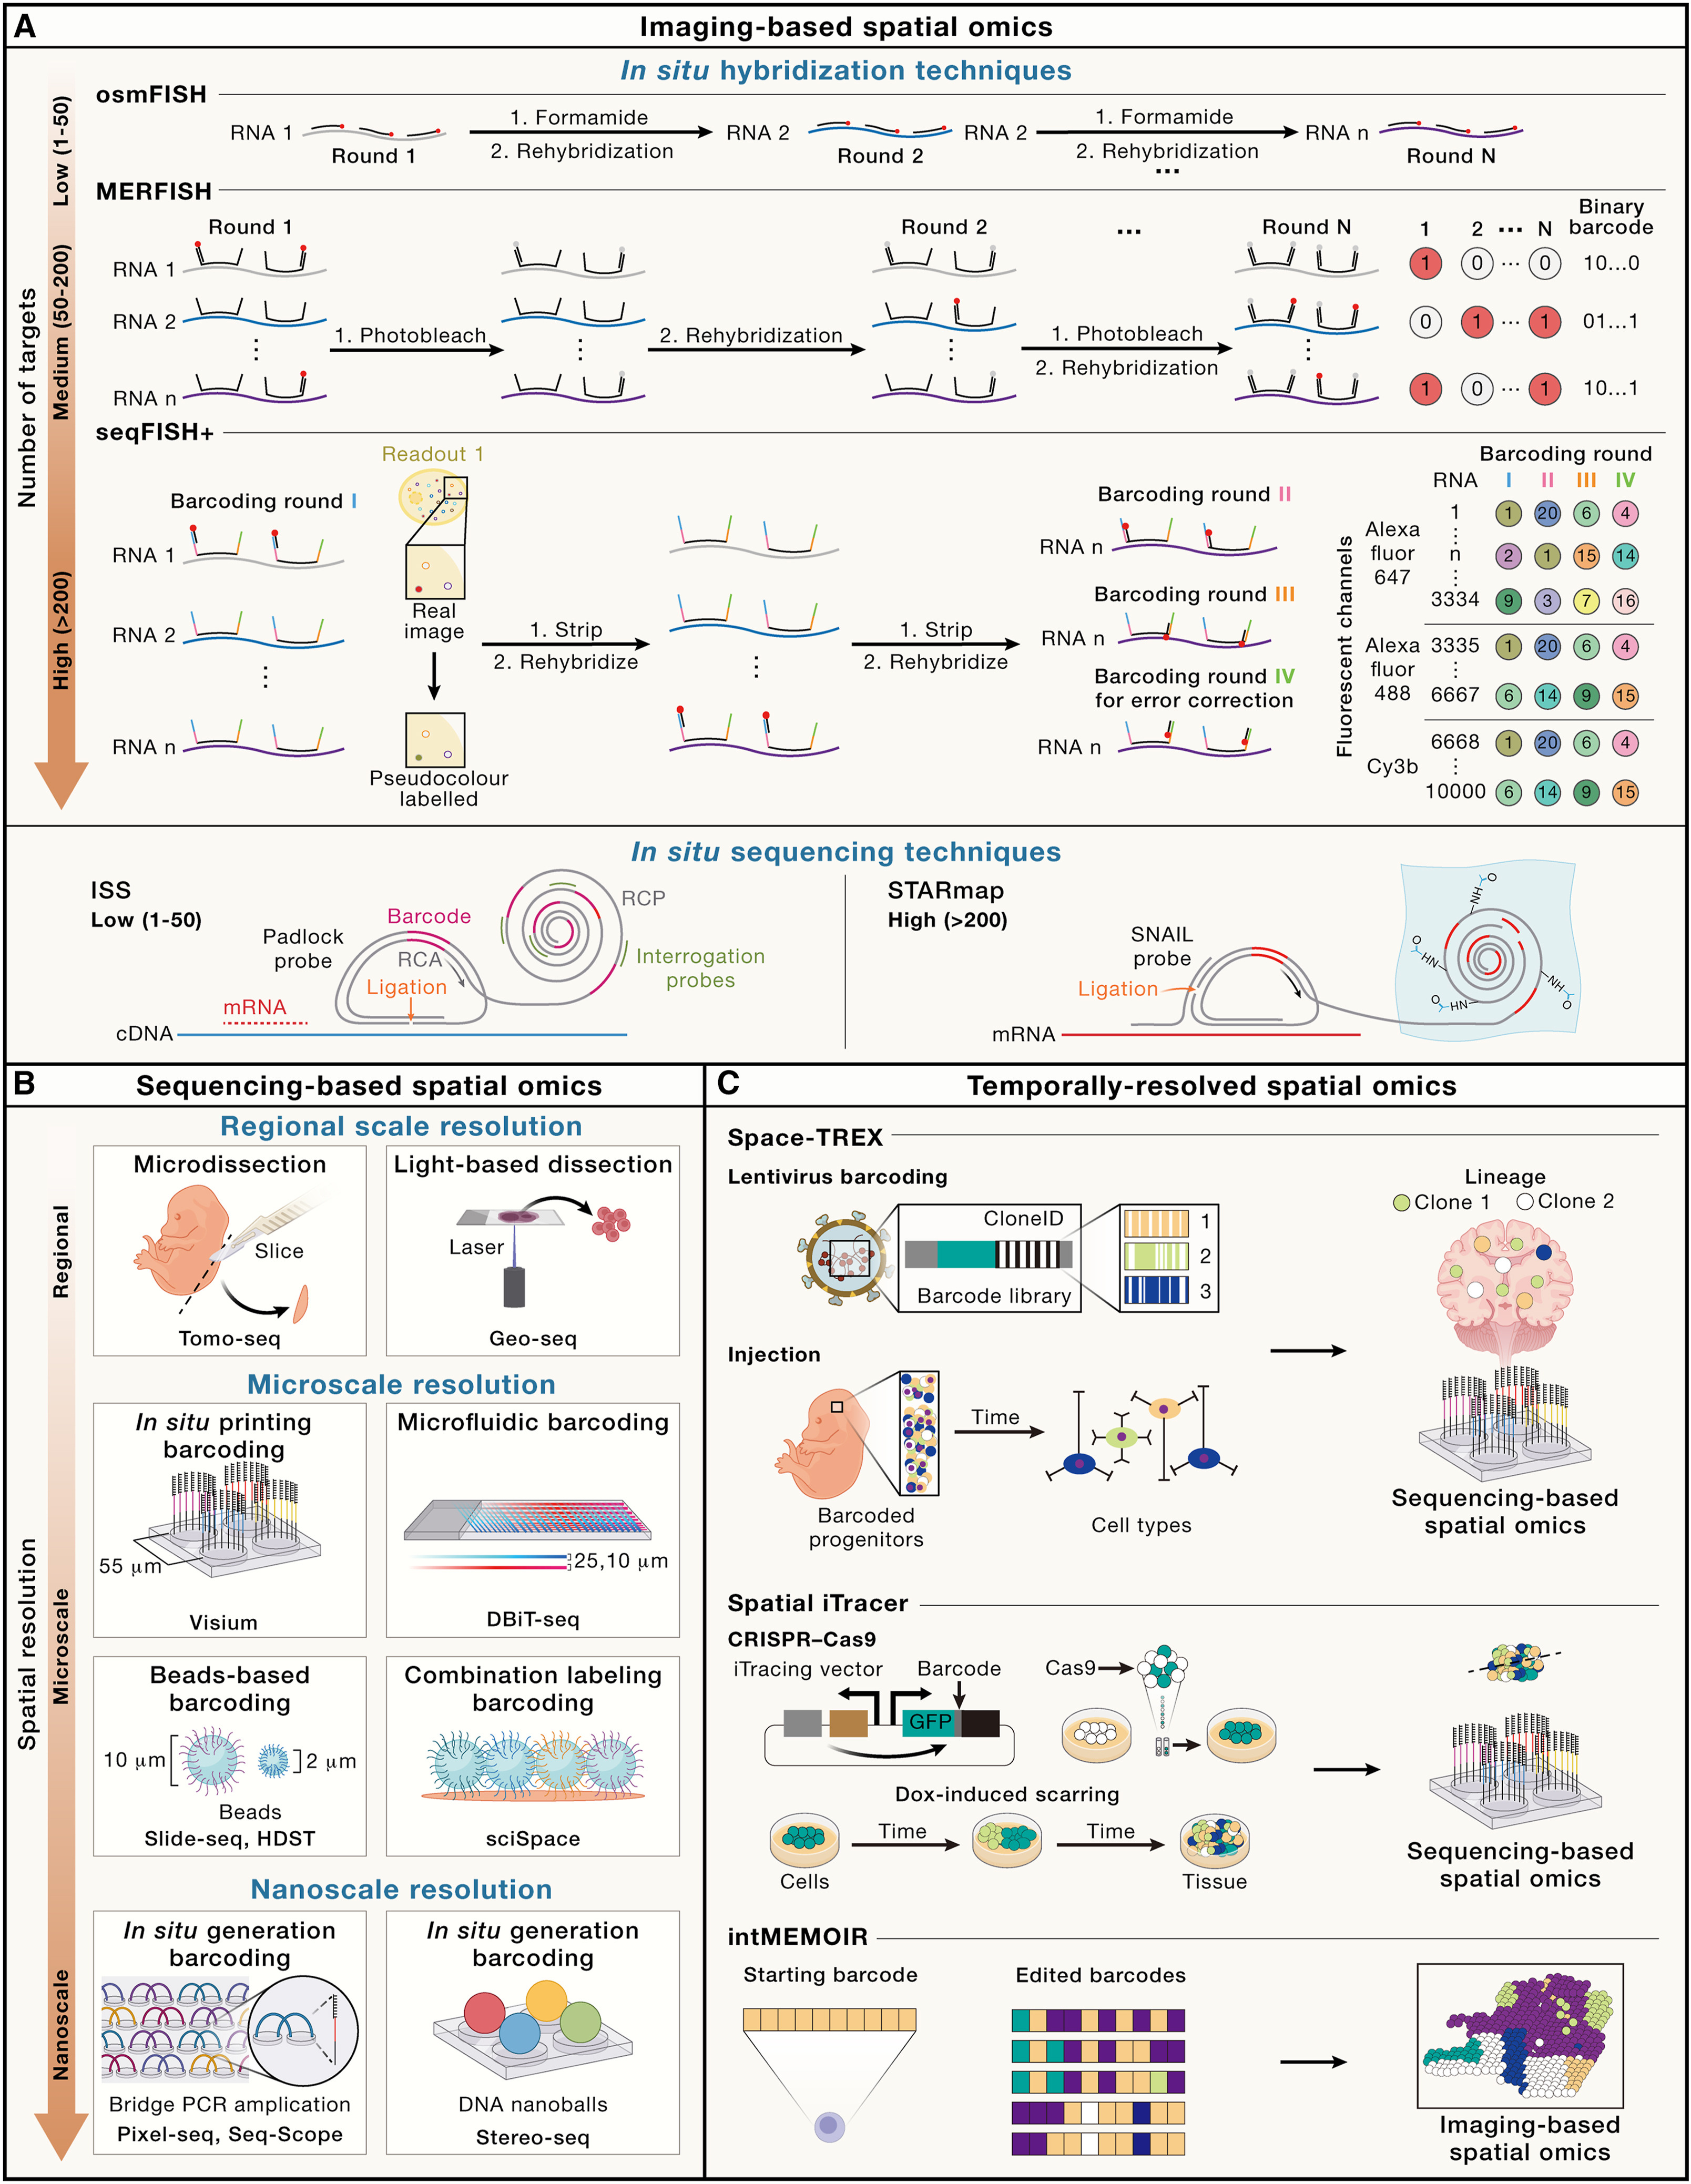
\includegraphics{./figs/spatialtech/Spatial omics technologies.jpg}
\caption{Spatial omics technologies}
\end{figure}

\hypertarget{spatial-transcriptomics-methods}{%
\section{Spatial transcriptomics Methods}\label{spatial-transcriptomics-methods}}

\begin{itemize}
\tightlist
\item
  Readinglist
\end{itemize}

\href{https://www.nature.com/articles/s41571-024-00926-7}{Spatial landscapes of cancers: insights and opportunities}

\href{https://www.nature.com/articles/s41571-024-00926-7.epdf?sharing_token=GNc_eiAuNQQXXGFjfD7Kz9RgN0jAjWel9jnR3ZoTv0MHjcqFYhINxQ2qcmoTpEHzNQAj3O3rn9odrZBd_LDLTzvupF49PpdT1TuLQEFlMTPjoCpw5MPA4eKqU39OI50crmunb320YA8fJd1osn9issYG6VPFpJJgFhZwbd54b7g\%3D}{shared link}

\begin{figure}
\centering
\includegraphics{./figs/spatialtech/Overview of single-cell and spatial transcriptomics.webp}
\caption{Overview of single-cell and spatial transcriptomics}
\end{figure}

\href{https://www.nature.com/articles/s41592-024-02325-3}{Systematic comparison of sequencing-based spatial transcriptomic methods}

\begin{figure}
\centering
\includegraphics{./figs/spatialtech/spatialmethodscomparasion.webp}
\caption{spatialmethodscomparasion}
\end{figure}

\hypertarget{spatial-datasets-collection}{%
\section{Spatial Datasets Collection}\label{spatial-datasets-collection}}

\begin{itemize}
\tightlist
\item
  CNA focused exploration
\end{itemize}

\begin{enumerate}
\def\labelenumi{\arabic{enumi}.}
\tightlist
\item
  DMG+GBM Dataset
\end{enumerate}

\href{https://www.nature.com/articles/s41467-023-36707-6}{Spatial transcriptomics reveals niche-specific enrichment and vulnerabilities of radial glial stem-like cells in malignant gliomas}

Diffuse midline glioma-H3K27M mutant (DMG) and glioblastoma (GBM) are the most lethal brain tumors that primarily occur in pediatric and adult patients, respectively. Both tumors exhibit significant heterogeneity, shaped by distinct genetic/epigenetic drivers, transcriptional programs including RNA splicing, and microenvironmental cues in glioma niches. However, the spatial organization of cellular states and niche-specific regulatory programs remain to be investigated. Here, we perform a spatial profiling of DMG and GBM combining short- and long-read spatial transcriptomics, and single-cell transcriptomic datasets. We identify clinically relevant transcriptional programs, RNA isoform diversity, and multi-cellular ecosystems across different glioma niches. We find that while the tumor core enriches for oligodendrocyte precursor-like cells, radial glial stem-like (RG-like) cells are enriched in the neuron-rich invasive niche in both DMG and GBM. Further, we identify niche-specific regulatory programs for RG-like cells, and functionally confirm that FAM20C mediates invasive growth of RG-like cells in a neuron-rich microenvironment in a human neural stem cell derived orthotopic DMG model. Together, our results provide a blueprint for understanding the spatial architecture and niche-specific vulnerabilities of DMG and GBM\citep{ren2023spatial}.

\href{https://ngdc.cncb.ac.cn/gsa-human/browse/HRA001865}{data request}

\begin{figure}
\centering
\includegraphics{./figs/spatialDatasets/DMG_GBM_dataset.webp}
\caption{multi-layered\_GBM Graphical abstract}
\end{figure}

\begin{enumerate}
\def\labelenumi{\arabic{enumi}.}
\setcounter{enumi}{1}
\tightlist
\item
  GBM\_ST
\end{enumerate}

\href{https://www.sciencedirect.com/science/article/pii/S1535610822002203?ref=pdf_download\&fr=RR-2\&rr=82a4735d0c8f20e1}{Spatially resolved multi-omics deciphers bidirectional tumor-host interdependence in glioblastoma}

\textbf{Summary}
Glioblastomas are malignant tumors of the central nervous system hallmarked by subclonal diversity and dynamic adaptation amid developmental hierarchies. The source of dynamic reorganization within the spatial context of these tumors remains elusive. Here, we characterized glioblastomas by spatially resolved transcriptomics, metabolomics, and proteomics. By deciphering regionally shared transcriptional programs across patients, we infer that glioblastoma is organized by spatial segregation of lineage states and adapts to inflammatory and/or metabolic stimuli, reminiscent of the reactive transformation in mature astrocytes. Integration of metabolic imaging and imaging mass cytometry uncovered locoregional tumor-host interdependence, resulting in spatially exclusive adaptive transcriptional programs. Inferring copy-number alterations emphasizes a spatially cohesive organization of subclones associated with reactive transcriptional programs, confirming that environmental stress gives rise to selection pressure. A model of glioblastoma stem cells implanted into human and rodent neocortical tissue mimicking various environments confirmed that transcriptional states originate from dynamic adaptation to various environments\citep{ravi2022spatially}.

\begin{figure}
\centering
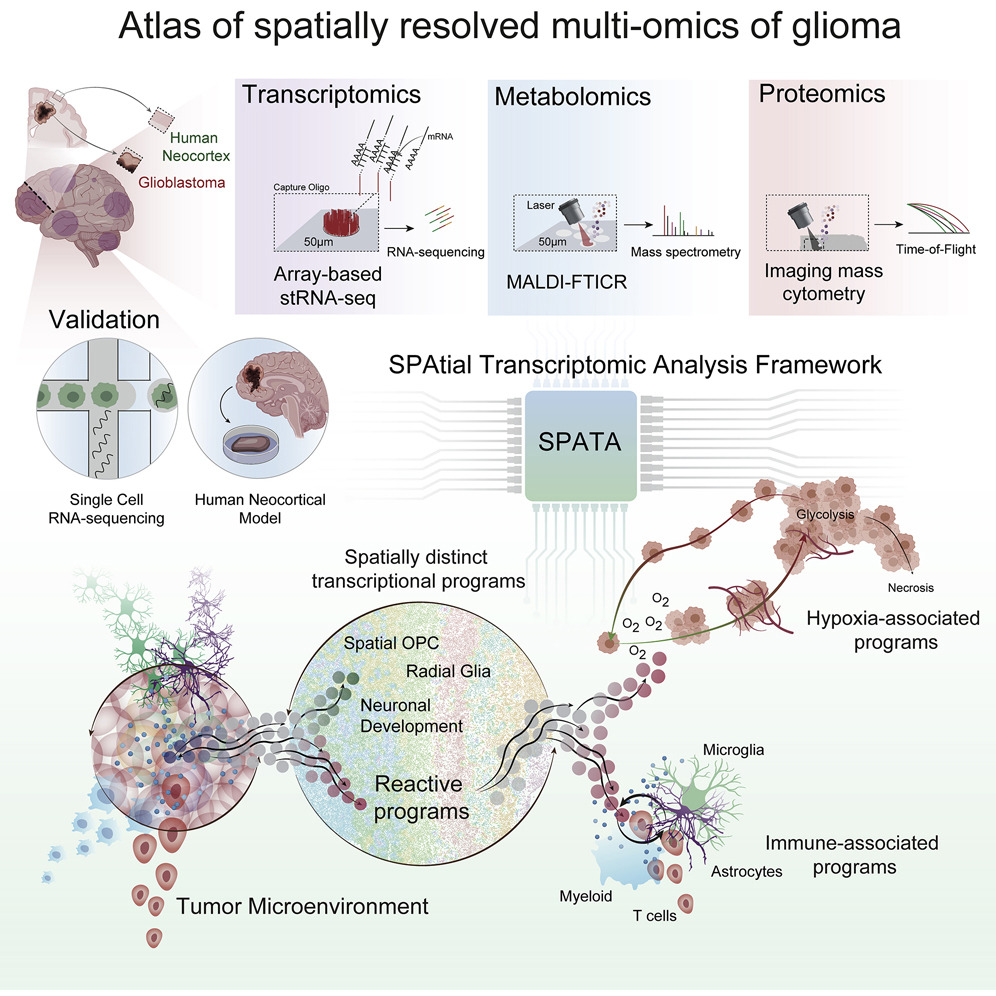
\includegraphics{./figs/spatialDatasets/multi-omicsGBM.jpg}
\caption{multi-layered\_GBM Graphical abstract}
\end{figure}

\textbf{Highlights}

\begin{itemize}
\item
  Five spatially distinct transcriptional programs are identified in glioblastomas
\item
  Hypoxia induces defined transcriptional and genomic responses, including CNAs
\item
  Immunosuppressive tumor-myeloid cell interactions are enhanced in segregated niches
\item
  Non-stress environments support subtype transition towards developmental stages
\end{itemize}

\begin{enumerate}
\def\labelenumi{\arabic{enumi}.}
\setcounter{enumi}{2}
\tightlist
\item
  GBM\_Multilayer
\end{enumerate}

\href{https://www.cell.com/cell/fulltext/S0092-8674(24)00320-9?_returnURL=https\%3A\%2F\%2Flinkinghub.elsevier.com\%2Fretrieve\%2Fpii\%2FS0092867424003209\%3Fshowall\%3Dtrue}{Integrative spatial analysis reveals a multi-layered organization of glioblastoma}

\textbf{Abstract}

Glioma contains malignant cells in diverse states. Here, we combine spatial transcriptomics, spatial proteomics, and computational approaches to define glioma cellular states and uncover their organization. We find three prominent modes of organization. First, gliomas are composed of small local environments, each typically enriched with one major cellular state. Second, specific pairs of states preferentially reside in proximity across multiple scales. This pairing of states is consistent across tumors. Third, these pairwise interactions collectively define a global architecture composed of five layers. Hypoxia appears to drive the layers, as it is associated with a long-range organization that includes all cancer cell states. Accordingly, tumor regions distant from any hypoxic/necrotic foci and tumors that lack hypoxia such as low-grade IDH-mutant glioma are less organized. In summary, we provide a conceptual framework for the organization of cellular states in glioma, highlighting hypoxia as a long-range tissue organizer.\citep{greenwald2024integrative}

Keywords: glioblastoma; glioma; hypoxia; intratumor heterogeneity; spatial proteomics; spatial transcriptomics.

\begin{figure}
\centering
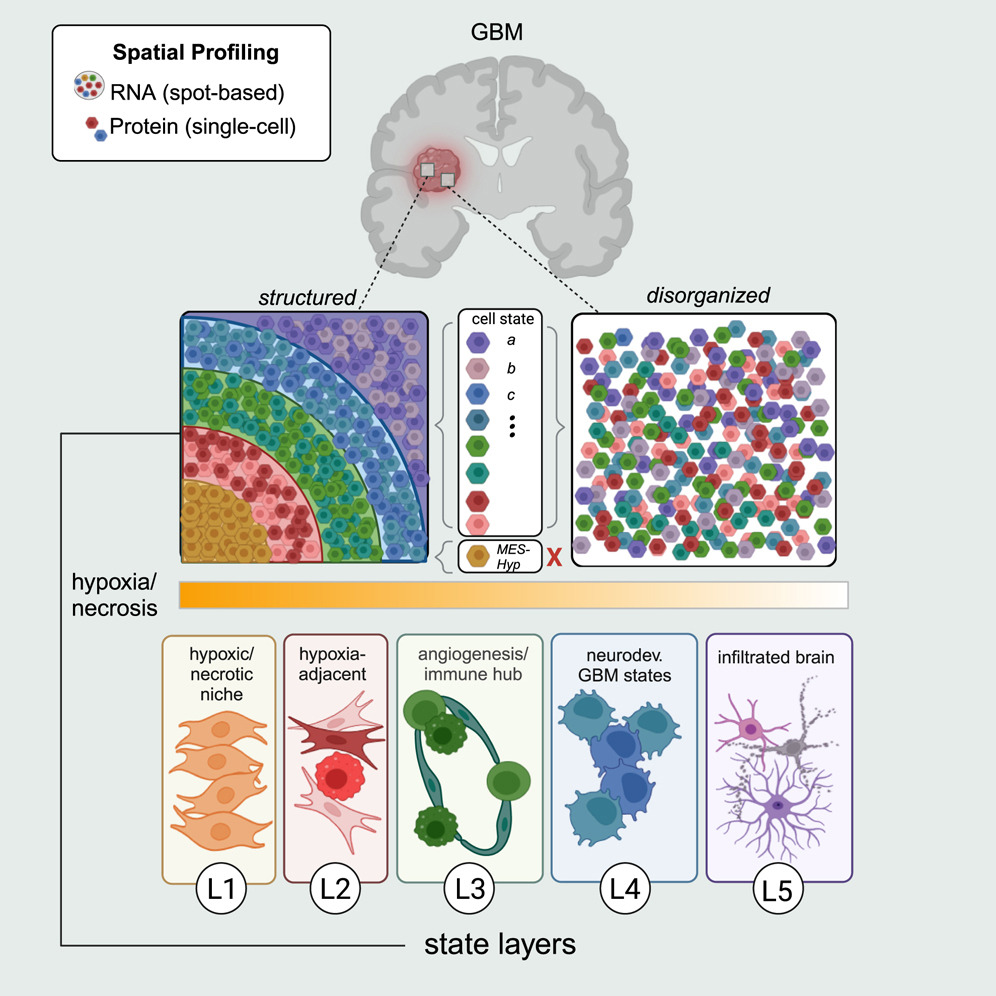
\includegraphics{./figs/spatialDatasets/multi-layered_GBM.jpg}
\caption{multi-layered\_GBM Graphical abstract}
\end{figure}

\textbf{Experimental model and study participant details}

Tumor samples used for Visium spatial transcriptomics and CODEX were obtained from patients undergoing tumor resection at University Hospital Zurich, Zurich, Switzerland (ZH samples), Massachusetts General Hospital, Boston, MA (MGH samples), and Brigham and Women's Hospital, Boston, MA (BWH samples) carried out in accordance with approved guidelines and with patient written consent under ethics approval KEK-ZH-Nr. 2015-0163, University Hospital Zurich, IRB \#10-417, Dana Farber Cancer Institute, and IRB \#1360-1, Weizmann Institute of Science. The clinical characteristics of the patient cohort are detailed in \href{https://www.cell.com/cms/10.1016/j.cell.2024.03.029/attachment/89b1c464-df78-4b1d-b0c4-22ff214799c7/mmc1}{Table S1}. \textbf{Tumors ZH1007, ZH1019, ZH881, ZH916, and ZH1041} were spatially annotated by the surgeon during navigated-guided surgery. In these cases, multiple samples were collected from different regions of the same tumor annotated as \textbf{necrotic, T1 contrast-enhancing, infiltrating, or bulk}. Equal numbers of samples from males and females were used in this study (n=17 of each).

\textbf{Recurrent patterns of expression heterogeneity across gliomas}

We identified 14 GBM spatial MPs, including \textbf{eight malignant and six non-malignant programs}, each reflecting a cancer cell state or non-malignant cell type (Figures 2C and 2D; Table S2). \textbf{Non-malignant MPs included Mac (macrophage/microglia) and Inflammatory-Mac (inflammatory macrophage/neutrophil), Oligo (oligodendrocyte), Vasc (endothelial cells and pericytes), Neuron, and Reactive-Ast (reactive astrocyte).} The latter included classical astrocytic markers (e.g., AGT and GJA1) and additional markers suggesting a reactive astrocytic state (e.g., metallothioneins). \textbf{Of the eight malignant MPs, five directly map to the single-cell GBM states: MES-hypoxia (MES2), MES (MES1), NPC-like, OPC-like, and AC-like (Figures 2D and S2G). }As expected, the neurodevelopmental-related malignant MPs (NPC-like, OPC-like, and AC-like) had high gene overlap with signatures of the respective non-malignant cell-type signatures, as also seen for the respective MPs derived from scRNA-seq (Figure S2H).
\textbf{The three additional malignant spatial MPs include}: (1) an astrocytic-like mesenchymal MP (\textbf{MES-Ast}) with enrichment of genes associated with glioma tumor microtubes (e.g., GAP43, KCNF1, and PTN) (Figure S2I);24,25,26 (2) proliferation and metabolism (\textbf{Prolif-Metab}), enriched with proliferation-related (e.g., CTNNB1, CNTD1, and TP53) and metabolism (e.g., SLC16A1 {[}MCT1{]}, GGCX, and PHGK1) genes; and (3) chromatin regulation (\textbf{Chromatin-Reg}), enriched with chromatin and transcriptional regulators (e.g., ATRX, KMT2E, BRD4, and SOX4), as well as with NPC-related genes (Figure S2J). Re-analysis of GBM scRNA-seq data supports these MPs as representing rare cellular states with partial similarity to previously defined states (Figures S2K, S2L, and S3A) and further shows that MES-Ast represents a unique state and not the simple combination of colocalized MES-like and AC-like cancer cells (Figure S3B).

\begin{enumerate}
\def\labelenumi{\arabic{enumi}.}
\setcounter{enumi}{3}
\tightlist
\item
  Liver
\end{enumerate}

\href{https://www.science.org/doi/10.1126/sciadv.abg3750}{Comprehensive analysis of spatial architecture in primary liver cancer}

Heterogeneity is the major challenge for cancer prevention and therapy. Here, we first constructed high-resolution spatial transcriptomes of primary liver cancers (PLCs) containing 84,823 spots within 21 tissues from seven patients. The progressive comparison of spatial tumor microenvironment (TME) characteristics from nontumor to leading-edge to tumor regions revealed that the tumor capsule potentially affects intratumor spatial cluster continuity, transcriptome diversity, and immune cell infiltration. Locally, we found that the bidirectional ligand-receptor interactions at the 100-μm-wide cluster-cluster boundary contribute to maintaining intratumor architecture and the PROM1+ and CD47+ cancer stem cell niches are related to TME remodeling and tumor metastasis. Last, we proposed a TLS-50 signature to accurately locate tertiary lymphoid structures (TLSs) spatially and unveiled that the distinct composition of TLSs is shaped by their distance to tumor cells. Our study provides previous unknown insights into the diverse tumor ecosystem of PLCs and has potential benefits for cancer intervention.\citep{wu2021comprehensive}

\href{https://ngdc.cncb.ac.cn/gsa-human/browse/HRA000437}{data request}

\begin{figure}
\centering
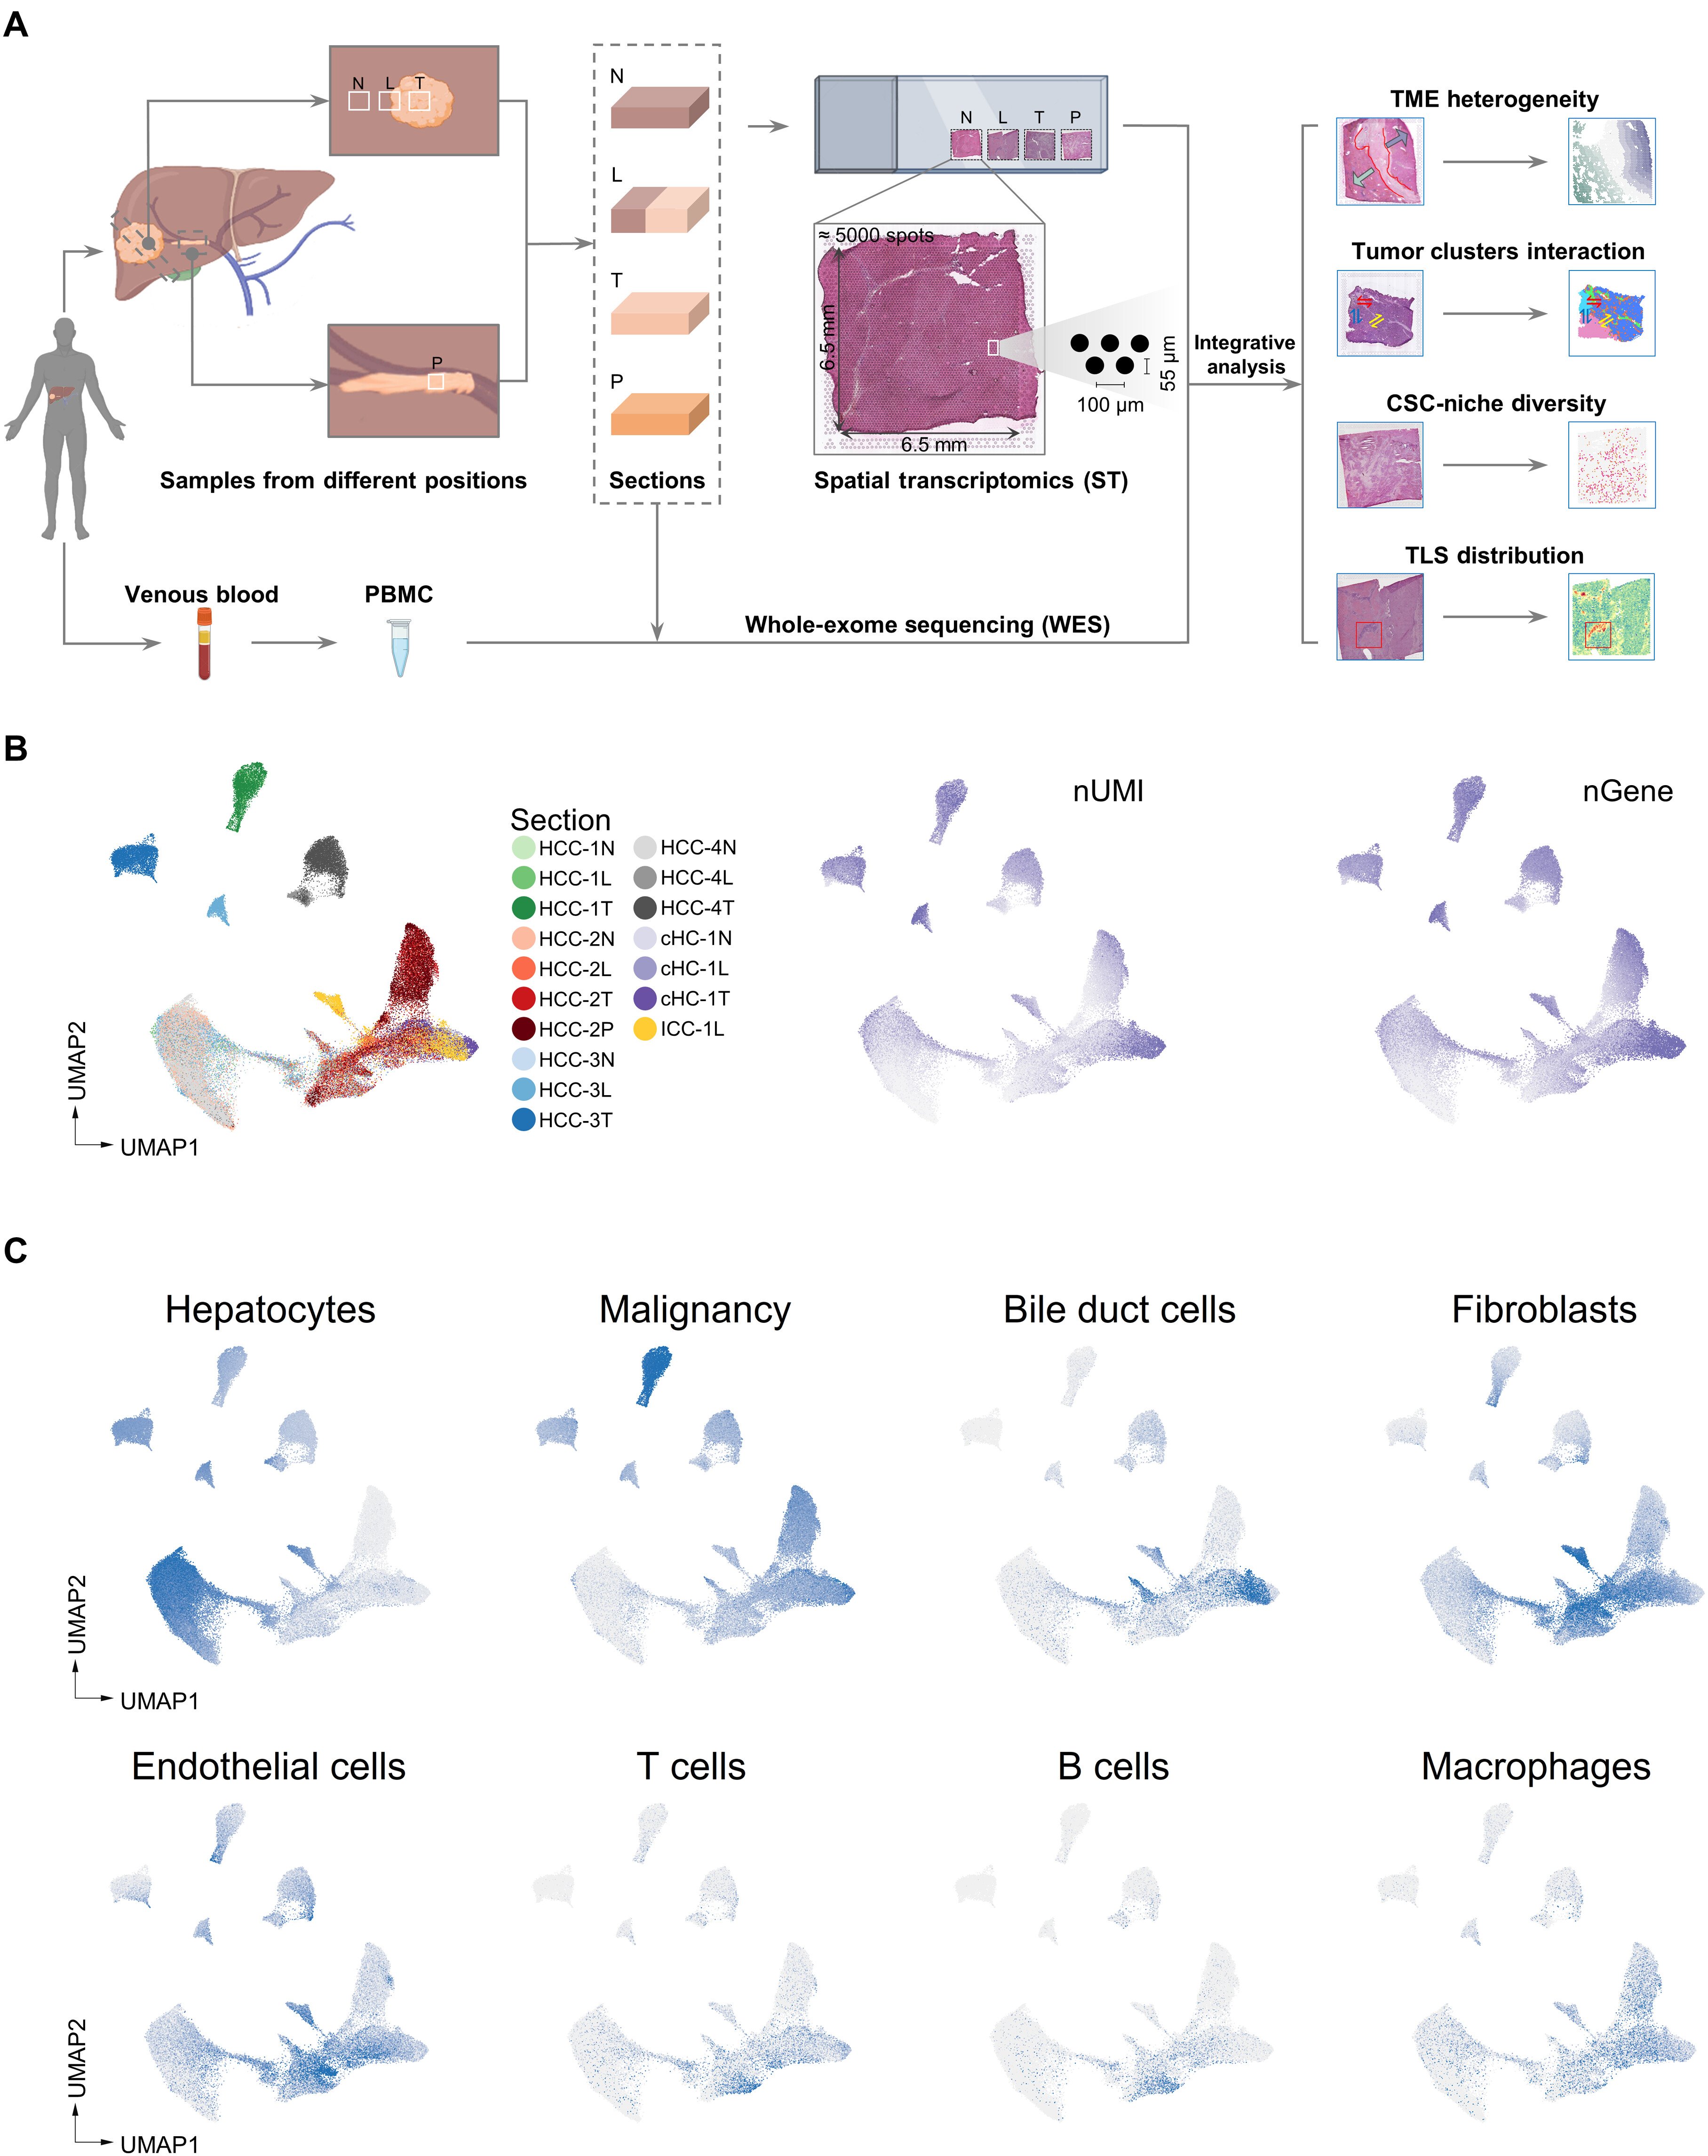
\includegraphics{./figs/spatialDatasets/sciadv.abg3750-f1.jpg}
\caption{Liver cancer fig1}
\end{figure}

\begin{enumerate}
\def\labelenumi{\arabic{enumi}.}
\setcounter{enumi}{4}
\tightlist
\item
  NPC
\end{enumerate}

\href{https://www.nature.com/articles/s41467-023-37614-6}{Nasopharyngeal carcinoma cells promote regulatory T cell development and suppressive activity via CD70-CD27 interaction}

\textbf{Abstract}
Despite the intense CD8+ T-cell infiltration in the tumor microenvironment of nasopharyngeal carcinoma, anti-PD-1 immunotherapy shows an unsatisfactory response rate in clinical trials, hindered by immunosuppressive signals. To understand how microenvironmental characteristics alter immune homeostasis and limit immunotherapy efficacy in nasopharyngeal carcinoma, here we establish a multi-center single-cell cohort based on public data, containing 357,206 cells from 50 patient samples. We reveal that nasopharyngeal carcinoma cells enhance development and suppressive activity of regulatory T cells via CD70-CD27 interaction. CD70 blocking reverts Treg-mediated suppression and thus reinvigorate CD8+ T-cell immunity. Anti-CD70+ anti-PD-1 therapy is evaluated in xenograft-derived organoids and humanized mice, exhibiting an improved tumor-killing efficacy. Mechanistically, CD70 knockout inhibits a collective lipid signaling network in CD4+ naive and regulatory T cells involving mitochondrial integrity, cholesterol homeostasis, and fatty acid metabolism. Furthermore, ATAC-Seq delineates that CD70 is transcriptionally upregulated by NFKB2 via an Epstein-Barr virus-dependent epigenetic modification. Our findings identify CD70+ nasopharyngeal carcinoma cells as a metabolic switch that enforces the lipid-driven development, functional specialization and homeostasis of Tregs, leading to immune evasion. This study also demonstrates that CD70 blockade can act synergistically with anti-PD-1 treatment to reinvigorate T-cell immunity against nasopharyngeal carcinoma \citep{gong2023nasopharyngeal}.

\begin{figure}
\centering
\includegraphics{./figs/spatialDatasets/NPC_Fig2_HTML.webp}
\caption{npc cancer fig2c}
\end{figure}

\begin{enumerate}
\def\labelenumi{\arabic{enumi}.}
\setcounter{enumi}{5}
\tightlist
\item
  Prostate
\end{enumerate}

\href{https://www.nature.com/articles/s41586-022-05023-2}{Spatially resolved clonal copy number alterations in benign and malignant tissue}

Defining the transition from benign to malignant tissue is fundamental to improving early diagnosis of cancer1. Here we use a systematic approach to study spatial genome integrity in situ and describe previously unidentified clonal relationships. We used spatially resolved transcriptomics2 to infer spatial copy number variations in \textgreater120,000 regions across multiple organs, in benign and malignant tissues. We demonstrate that genome-wide copy number variation reveals distinct clonal patterns within tumours and in nearby benign tissue using an organ-wide approach focused on the prostate. Our results suggest a model for how genomic instability arises in histologically benign tissue that may represent early events in cancer evolution. We highlight the power of capturing the molecular and spatial continuums in a tissue context and challenge the rationale for treatment paradigms, including focal therapy.\citep{erickson2022spatially}

\begin{figure}
\centering
\includegraphics{./figs/spatialDatasets/prostate_Fig1_HTML.webp}
\caption{prostate cancer fig1}
\end{figure}

\begin{enumerate}
\def\labelenumi{\arabic{enumi}.}
\setcounter{enumi}{6}
\tightlist
\item
  Skin
\end{enumerate}

\href{https://www.cell.com/cell/fulltext/S0092-8674(20)30672-3?_returnURL=https\%3A\%2F\%2Flinkinghub.elsevier.com\%2Fretrieve\%2Fpii\%2FS0092867420306723\%3Fshowall\%3Dtrue}{Multimodal Analysis of Composition and Spatial Architecture in Human Squamous Cell Carcinoma}

\begin{figure}
\centering
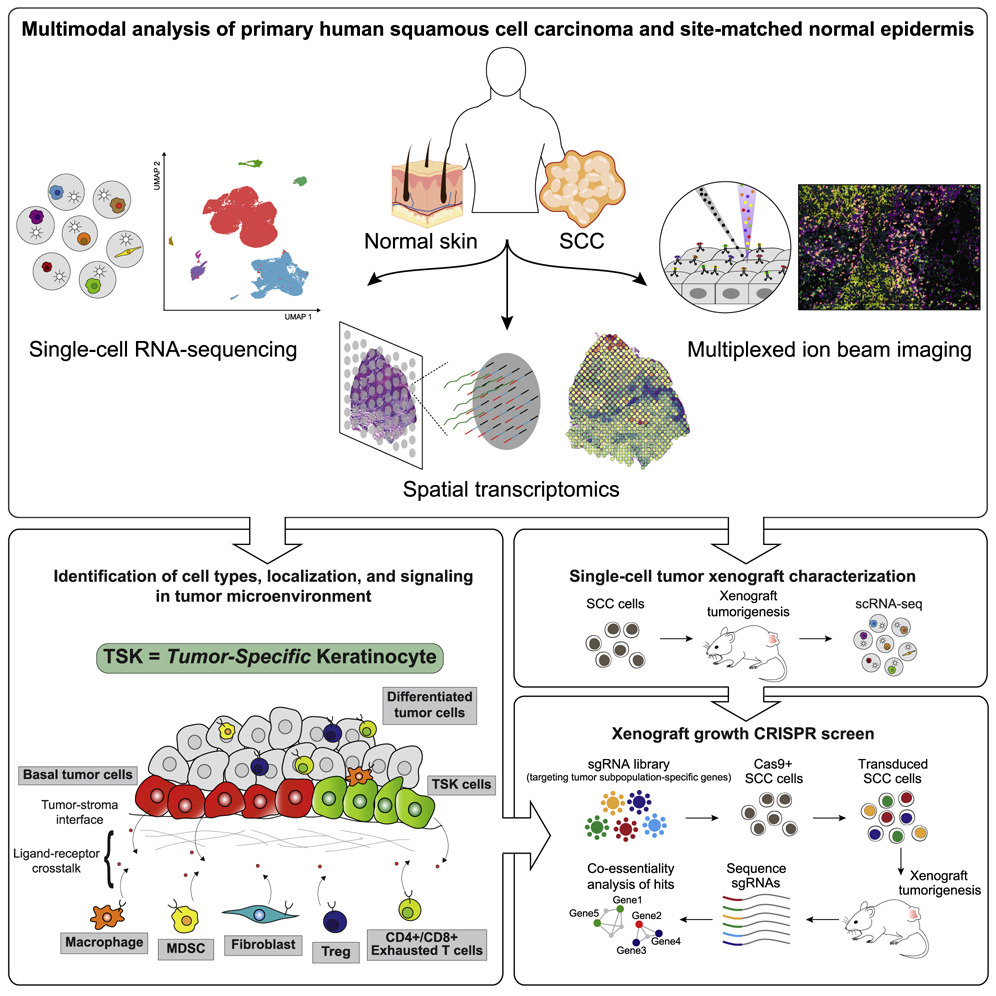
\includegraphics{./figs/spatialDatasets/Skin Graphical Abstract.jpg}
\caption{prostate cancer fig1}
\end{figure}

\textbf{Highlights}

\begin{itemize}
\item
  Profiling of 10 human skin SCCs and matched normals via scRNA-seq, ST, and MIBI
\item
  Tumor-specific keratinocytes (TSKs) reside within a fibrovascular niche at leading edges
\item
  Distinct ligand-receptor and spatial niche associations for tumor and stromal cells.
\item
  Subpopulation essential tumorigenic gene networks defined by in vivo CRISPR screening
\end{itemize}

\textbf{Summary}
To define the cellular composition and architecture of cutaneous squamous cell carcinoma (cSCC), we combined single-cell RNA sequencing with spatial transcriptomics and multiplexed ion beam imaging from a series of human cSCCs and matched normal skin. cSCC exhibited four tumor subpopulations, three recapitulating normal epidermal states, and a tumor-specific keratinocyte (TSK) population unique to cancer, which localized to a fibrovascular niche. Integration of single-cell and spatial data mapped ligand-receptor networks to specific cell types, revealing TSK cells as a hub for intercellular communication. Multiple features of potential immunosuppression were observed, including T regulatory cell (Treg) co-localization with CD8 T cells in compartmentalized tumor stroma. Finally, single-cell characterization of human tumor xenografts and in vivo CRISPR screens identified essential roles for specific tumor subpopulation-enriched gene networks in tumorigenesis. These data define cSCC tumor and stromal cell subpopulations, the spatial niches where they interact, and the communicating gene networks that they engage in cancer\citep{ji2020multimodal}.

\hypertarget{d-biology}{%
\section{3D biology}\label{d-biology}}

\hypertarget{sequencing-data-relative-knowledge}{%
\section{Sequencing data relative Knowledge}\label{sequencing-data-relative-knowledge}}

\hypertarget{image-data-relative-knowledge}{%
\section{Image data relative Knowledge}\label{image-data-relative-knowledge}}

\hypertarget{proteomics}{%
\chapter{Proteomics}\label{proteomics}}

\hypertarget{ptm-cross-talk}{%
\section{PTM cross-talk}\label{ptm-cross-talk}}

\hypertarget{ptm-cluster}{%
\section{PTM Cluster}\label{ptm-cluster}}

\hypertarget{ptm-and-cancer}{%
\section{PTM and cancer}\label{ptm-and-cancer}}

\hypertarget{protein-structure}{%
\section{Protein structure}\label{protein-structure}}

\hypertarget{protein-folding-prediction-background}{%
\subsection{Protein Folding Prediction Background}\label{protein-folding-prediction-background}}

\hypertarget{introduction}{%
\subsubsection{introduction}\label{introduction}}

\begin{itemize}
\item
  How to record a protein structue
\item
  What to predict
\end{itemize}

\hypertarget{methods}{%
\subsubsection{methods}\label{methods}}

\begin{itemize}
\tightlist
\item
  ReceptorX
\item
  ReceptorX-d
\item
  trRosetta
\item
  AlphaFold1
\item
  AlphaFold2
\end{itemize}

\hypertarget{deep-learing-in-protein-structure-prediction}{%
\subsubsection{deep learing in protein structure prediction}\label{deep-learing-in-protein-structure-prediction}}

\hypertarget{epigenomics}{%
\chapter{Epigenomics}\label{epigenomics}}

\hypertarget{pubmon-1}{%
\chapter{Pubmon}\label{pubmon-1}}

\hypertarget{phd-year-1}{%
\section{2020-2021 PhD year 1}\label{phd-year-1}}

-202009

-202010

-202011

-202012

-202101

-202102

-202103

-202104

-202105

-202106

-202107

-202108

\hypertarget{phd-year-2}{%
\section{2021-2022 PhD year 2}\label{phd-year-2}}

The cell-level resolution data provide much richer information for answering a number of important questions that cannot otherwise be answered by bulk data, for example, the composition of cell types in complex tissues, the cell-to-cell heterogeneity in transcription, and the transcriptional dynamics in many biological processes such as development, differentiation, and disease progression.

There are several scientific goals in scRNA-seq studies. The first one is to decipher the cellular composition of complex tissues: one wants to know the identities of the cell types and subtypes, as well as their proportions in the tissue sample. The cellular composition itself can be of great interest in biological and clinical practices, for example, it was reported that tumor-infiltrating immune cell compositions play a vital role in understanding antitumor immune responses {[}4{]}. Once the cell types are identified, cell type--specific gene expressions are also of great interest since they enhance the understandings of cell signatures {[}5{]}. There are other goals, for example, new and rare cell type discovery {[}6{]} and pseudo-time construction to represent the temporal dynamics of transcription during a biological process {[}7{]}.

\begin{itemize}
\tightlist
\item
  202109
\end{itemize}

\textbf{\href{https://genomebiology.biomedcentral.com/articles/10.1186/s13059-021-02480-2}{Evaluation of some aspects in supervised cell type identification for single-cell RNA-seq: classifier, feature selection, and reference construction}\citep{ma2021evaluation}}

\textbf{Background}
Cell type identification is one of the most important questions in single-cell RNA sequencing (scRNA-seq) data analysis. With the accumulation of public scRNA-seq data, supervised cell type identification methods have gained increasing popularity due to better accuracy, robustness, and computational performance. Despite all the advantages, the performance of the supervised methods relies heavily on several key factors: feature selection, prediction method, and, most importantly, choice of the reference dataset.

\textbf{Results}
In this work, we perform extensive real data analyses to systematically evaluate these strategies in supervised cell identification. We first benchmark nine classifiers along with six feature selection strategies and investigate the impact of reference data size and number of cell types in cell type prediction. Next, we focus on how discrepancies between reference and target datasets and how data preprocessing such as imputation and batch effect correction affect prediction performance. We also investigate the strategies of pooling and purifying reference data.

\textbf{Conclusions}
Based on our analysis results, we provide guidelines for using supervised cell typing methods. We suggest combining all individuals from available datasets to construct the reference dataset and use multi-layer perceptron (MLP) as the classifier, along with F-test as the feature selection method. All the code used for our analysis is available on GitHub (\url{https://github.com/marvinquiet/RefConstruction_supervisedCelltyping}).

\begin{figure}
\centering
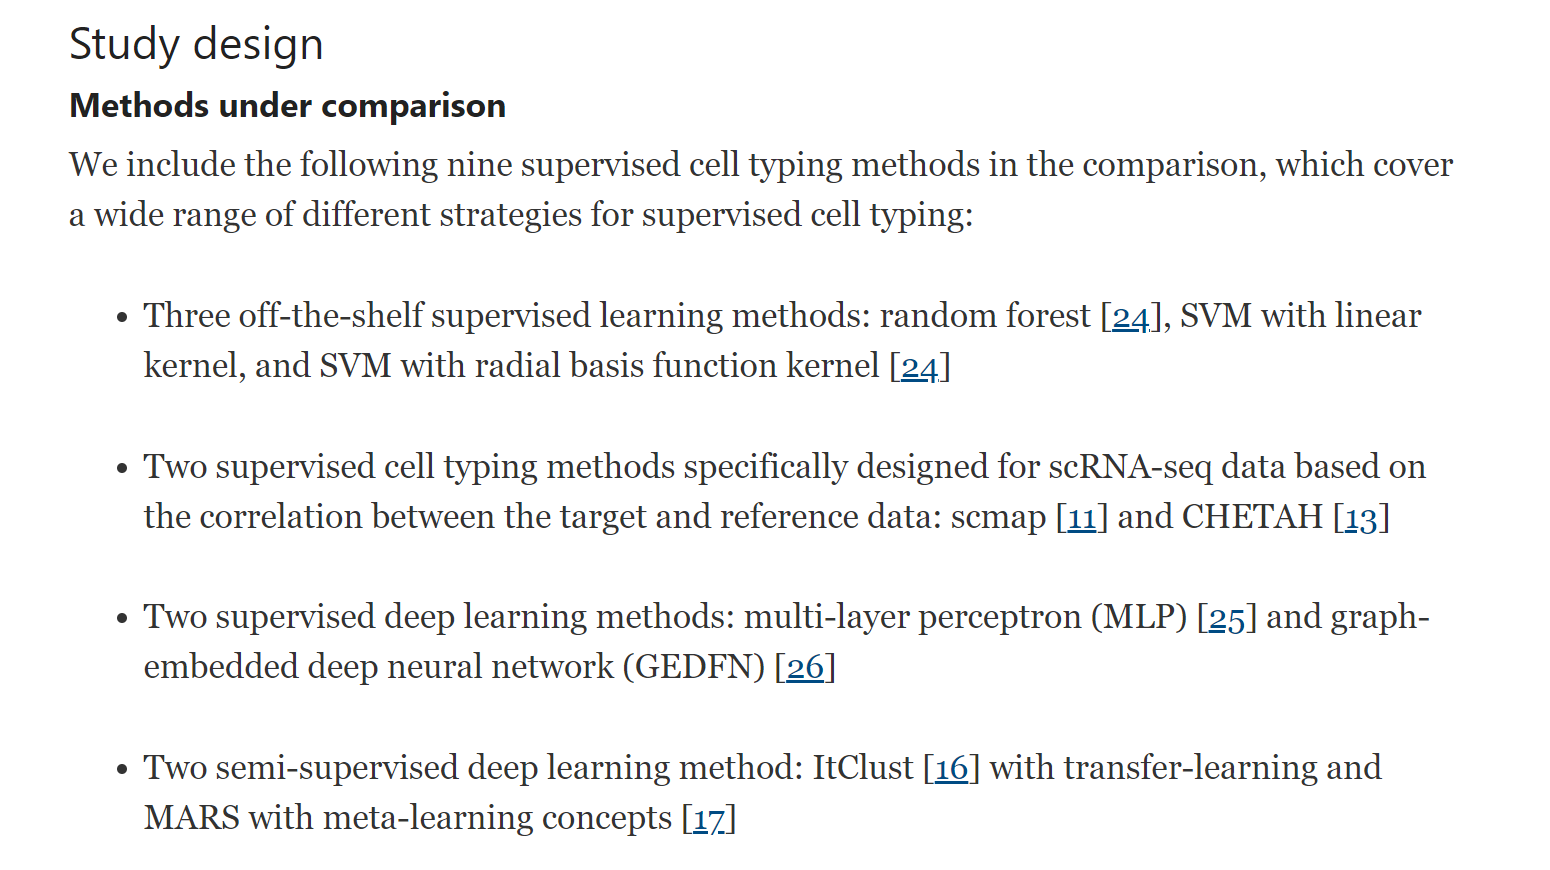
\includegraphics{./figs/pubmon/2021-2022/CELLTYPE_ANNO_BENCHMARK.png}
\caption{Study design}
\end{figure}

There are several other supervised cell typing methods available for scRNA-seq. For example, scSorter {[}27{]} borrows information from lowly expressed marker genes to assign cells; scPred {[}12{]} adopts a principal component analysis (PCA)-based feature selection; SingleCellNet {[}28{]} uses top-pair transformation on gene space and selects informative paired genes as features; CellAssign {[}29{]} builds a probabilistic model with some prior knowledge of cell markers, etc. But according to a recent comparison {[}20{]}, SVM with rejection, scmap, and CHEAH are among the best performers, so we decide not to include more such methods. GEDFN is a method designed for predicting phenotype from bulk expression but can be directly applied to scRNA-seq cell typing. We include it because we want to understand whether incorporating gene network information can improve the results. ItClust is a semi-supervised method which only uses the reference data to obtain initial values for unsupervised clustering in target data. MARS uses a meta-learning concept to construct cell type landmarks by jointly embedding both annotated and unannotated data without removing the batch effects and then assigns cell types based on the learned embedding space. We want to evaluate the performances of these semi-supervised methods under different scenarios.

\textbf{\href{https://genomebiology.biomedcentral.com/articles/10.1186/s13059-021-02478-w}{SUPERGNOVA: local genetic correlation analysis reveals heterogeneous etiologic sharing of complex traits}\citep{zhang2021supergnova}}

Local genetic correlation quantifies the genetic similarity of complex traits in specific genomic regions. However, accurate estimation of local genetic correlation remains challenging, due to linkage disequilibrium in local genomic regions and sample overlap across studies. We introduce SUPERGNOVA, a statistical framework to estimate local genetic correlations using summary statistics from genome-wide association studies. We demonstrate that SUPERGNOVA outperforms existing methods through simulations and analyses of 30 complex traits. In particular, we show that the positive yet paradoxical genetic correlation between autism spectrum disorder and cognitive performance could be explained by two etiologically distinct genetic signatures with bidirectional local genetic correlations.

\begin{figure}
\centering
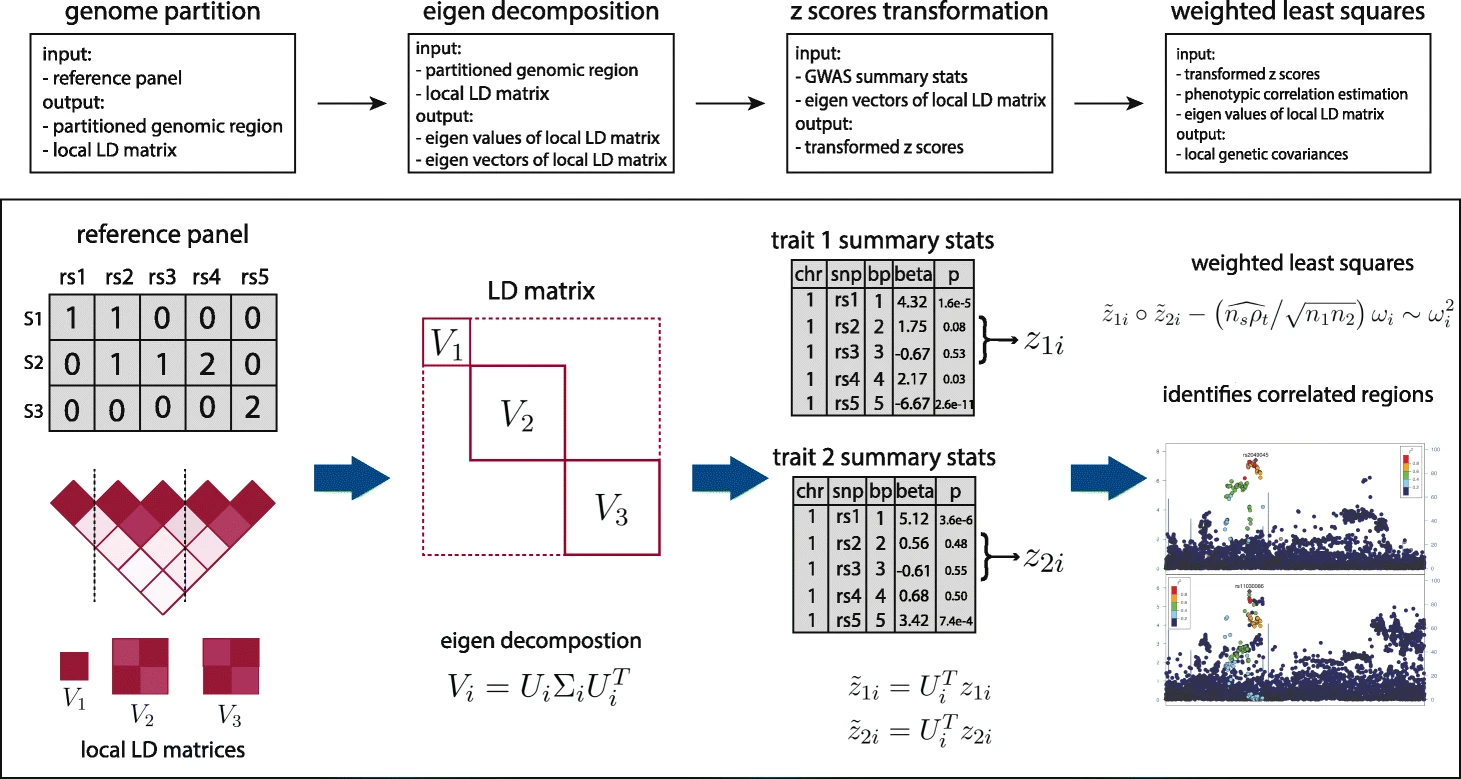
\includegraphics{./figs/pubmon/2021-2022/SUPERGNOVA_workflow.png}
\caption{SUPERGNOVA\_workflow}
\end{figure}

\textbf{\href{https://genomebiology.biomedcentral.com/articles/10.1186/s13059-021-02477-x}{Recovering genotypes and phenotypes using allele-specific genes}\citep{gursoy2021recovering}}

With the recent increase in RNA sequencing efforts using large cohorts of individuals, surveying allele-specific gene expression is becoming increasingly frequent. Here, we report that, despite not containing explicit variant information, a list of genes known to be allele-specific in an individual is enough to recover key variants and link the individuals back to their genotypes and phenotypes. This creates a privacy conundrum.

\textbf{\href{https://genomebiology.biomedcentral.com/articles/10.1186/s13059-021-02472-2}{NanoCaller for accurate detection of SNPs and indels in difficult-to-map regions from long-read sequencing by haplotype-aware deep neural networks}\citep{ahsan2021nanocaller}}

Long-read sequencing enables variant detection in genomic regions that are considered difficult-to-map by short-read sequencing. To fully exploit the benefits of longer reads, here we present a deep learning method NanoCaller, which detects SNPs using long-range haplotype information, then phases long reads with called SNPs and calls indels with local realignment. Evaluation on 8 human genomes demonstrates that NanoCaller generally achieves better performance than competing approaches. We experimentally validate 41 novel variants in a widely used benchmarking genome, which could not be reliably detected previously. In summary, NanoCaller facilitates the discovery of novel variants in complex genomic regions from long-read sequencing.

\begin{itemize}
\tightlist
\item
  202110
\end{itemize}

\href{https://www.nature.com/articles/d41586-021-02493-8}{A census of cell types in the brain's motor cortex}

\href{https://www.nature.com/articles/s41586-021-03950-0}{A multimodal cell census and atlas of the mammalian primary motor cortex}

\begin{itemize}
\tightlist
\item
  important
\end{itemize}

\textbf{\href{https://biccn.org/}{NIH's Brain Research through Advancing Innovative Neurotechnologies (BRAIN) Initiative - Cell Census Network (BICCN)}}

\hypertarget{todo-list}{%
\subsubsection{TODO List}\label{todo-list}}

\begin{itemize}
\tightlist
\item
  202204 todolist
\end{itemize}

\textbf{\href{https://www.biorxiv.org/content/10.1101/2022.04.09.487529v1}{Experimental evolution in TP53 deficient gastric organoids recapitulates tumorigenesis}\citep{karlsson2022experimental}}

\textbf{\href{https://www.nature.com/articles/s41587-022-01233-1}{Spatial charting of single-cell transcriptomes in tissues}\citep{wei2022spatial}}

two CNV papers

\textbf{\href{https://www.biorxiv.org/content/10.1101/2022.02.07.479314v1}{Haplotype-enhanced inference of somatic copy number profiles from single-cell transcriptomes}\citep{gao2022haplotype}}

\textbf{\href{https://www.biorxiv.org/content/10.1101/2021.06.04.447031v1}{Evolutionary tracking of cancer haplotypes at single-cell resolution}\citep{williams2021evolutionary}}

\hypertarget{resources}{%
\subsection{Resources}\label{resources}}

\textbf{\href{https://biccn.org/}{NIH's Brain Research through Advancing Innovative Neurotechnologies (BRAIN) Initiative - Cell Census Network (BICCN)}}

\hypertarget{ppi-topic}{%
\subsection{PPI topic}\label{ppi-topic}}

\href{https://mp.weixin.qq.com/s/EWLSD7wB-GUIXS94LtPtWQ}{identifying cancer drivers}

\hypertarget{phd-year-4}{%
\section{2023-2024 PhD year 4}\label{phd-year-4}}

\hypertarget{pre-postdoc}{%
\section{2024-2025 Pre Postdoc}\label{pre-postdoc}}

\href{https://www.cell.com/action/showPdf?pii=S0092-8674\%2824\%2901019-5}{Spatially exploring RNA biology in archival formalin-fixed paraffin-embedded tissues}

\href{https://www.biorxiv.org/content/10.1101/2024.12.15.628568v1}{Echidna: A Bayesian framework for quantifying gene dosage effect impacting phenotypic plasticity}

\hypertarget{method-of-the-year}{%
\chapter{Method of the Year}\label{method-of-the-year}}

\hypertarget{method-of-the-year-2022}{%
\section{Method of the Year 2022:}\label{method-of-the-year-2022}}

\hypertarget{method-of-the-year-2021-protein-structure-prediction}{%
\section{Method of the Year 2021: Protein structure prediction}\label{method-of-the-year-2021-protein-structure-prediction}}

\hypertarget{method-of-the-year-2020-spatially-resolved-transcriptomics}{%
\section{Method of the Year 2020: spatially resolved transcriptomics}\label{method-of-the-year-2020-spatially-resolved-transcriptomics}}

\hypertarget{method-of-the-year-2019-single-cell-multimodal-omics}{%
\section{Method of the Year 2019: Single-cell multimodal omics}\label{method-of-the-year-2019-single-cell-multimodal-omics}}

  \bibliography{book.bib,singelcell.bib,packages.bib,sources.bib,tech.bib,pubmon.bib,topic\_based.bib,datasets.bib}

\end{document}
